%%% Hlavní soubor. Zde se definují základní parametry a odkazuje se na ostatní části. %%%

% Meta-data o práci (je nutno upravit)
\input metadata.tex

% Vygenerujeme metadata ve formátu XMP pro použití balíčkem pdfx
\input xmp.tex

%% Verze pro jednostranný tisk:
% Okraje: levý 40mm, pravý 25mm, horní a dolní 25mm
% (ale pozor, LaTeX si k levému a hornímu sám přidává 1in=25.4mm)
% \documentclass[12pt,a4paper]{report}
% \setlength\textwidth{145mm}
% \setlength\textheight{247mm}
% \setlength\oddsidemargin{14.6mm}
% \setlength\evensidemargin{14.6mm}
% \setlength\topmargin{0mm}
% \setlength\headsep{0mm}
% \setlength\headheight{0mm}
% % \openright zařídí, aby následující text začínal na pravé straně knihy
% \let\openright=\clearpage

%% Pokud tiskneme oboustranně:
% \documentclass[12pt,a4paper,twoside,openright]{report}
% \setlength\textwidth{145mm}
% \setlength\textheight{247mm}
% \setlength\oddsidemargin{14.6mm}
% \setlength\evensidemargin{0mm}
% \setlength\topmargin{0mm}
% \setlength\headsep{0mm}
% \setlength\headheight{0mm}
% \let\openright=\cleardoublepage

%% Pokud práci odevzdáváme pouze elektronicky, vypadají lépe symetrické okraje
\documentclass[12pt,a4paper]{report}
\setlength\textwidth{145mm}
\setlength\textheight{247mm}
\setlength\oddsidemargin{7.1mm}
\setlength\evensidemargin{7.1mm}
\setlength\topmargin{0mm}
\setlength\headsep{0mm}
\setlength\headheight{0mm}
\let\openright=\clearpage

%% Vytváříme PDF/A-2u
\usepackage[a-2u]{pdfx}

%% Přepneme na českou sazbu a fonty Latin Modern
\usepackage[czech]{babel}
\usepackage{lmodern}

% Pokud nepouživáme LuaTeX, je potřeba ještě nastavit kódování znaků
\usepackage{iftex}
\ifpdftex
\usepackage[utf8]{inputenc}
\usepackage[T1]{fontenc}
\usepackage{textcomp}
\fi

%%% Další užitečné balíčky (jsou součástí běžných distribucí LaTeXu)
\usepackage{amsmath}        % rozšíření pro sazbu matematiky
\usepackage{amsfonts}       % matematické fonty
\usepackage{amsthm}         % sazba vět, definic apod.
\usepackage{bm}             % tučné symboly (příkaz \bm)
\usepackage{booktabs}       % lepší vodorovné linky v tabulkách
\usepackage{caption}        % umožní definovat vlastní popisky plovoucích objektů
\usepackage{csquotes}       % uvozovky závislé na jazyku
\usepackage{dcolumn}        % vylepšené zarovnání sloupců tabulek
\usepackage{floatrow}       % umožní definovat vlastní typy plovoucích objektů
\usepackage{graphicx}       % vkládání obrázků
\usepackage{icomma}         % inteligetní čárka v matematickém módu
\usepackage{indentfirst}    % zavede odsazení 1. odstavce kapitoly
\usepackage[nopatch=item]{microtype}  % mikrotypografická rozšíření
\usepackage{paralist}       % lepší enumerate a itemize
\usepackage[nottoc]{tocbibind} % zajistí přidání seznamu literatury,
                            % obrázků a tabulek do obsahu
\usepackage{xcolor}         % barevná sazba

% Balíček hyperref, kterým jdou vyrábět klikací odkazy v PDF,
% ale hlavně ho používáme k uložení metadat do PDF (včetně obsahu).
% Většinu nastavítek přednastaví balíček pdfx.
\hypersetup{unicode}
\hypersetup{breaklinks=true}

% Balíčky pro sazbu informatických prací
\usepackage{algpseudocode}  % součást balíčku algorithmicx
\usepackage[Algoritmus]{algorithm}
\usepackage{fancyvrb}       % vylepšené prostředí verbatim
\usepackage{listings}       % zvýrazňování syntaxe zdrojových textů

% Cleveref může zjednodušit odkazování, ale jeho užitečnost pro češtinu
% je minimalní, protože nezvládá skloňování.
% \usepackage{cleveref}

% Formátování bibliografie (odkazů na literaturu)
% Detailní nastavení můžete upravit v souboru macros.tex.
%
% POZOR: Zvyklosti různých oborů a kateder se liší. Konzultujte se svým
% vedoucím, jaký formát citací je pro vaši práci vhodný!
%
% Základní formát podle normy ISO 690 s číslovanými odkazy
\usepackage[natbib,style=iso-numeric,sorting=none]{biblatex}
% ISO 690 s alfanumerickými odkazy (zkratky jmen autorů)
%\usepackage[natbib,style=iso-alphabetic]{biblatex}
% ISO 690 s citacemi tvaru Autor (rok)
%\usepackage[natbib,style=iso-authoryear]{biblatex}
%
% V některých oborech je běžnější obyčejný formát s číslovanými odkazy
% (sorting=none říká, že se bibliografie má řadit podle pořadí citací):
%\usepackage[natbib,style=numeric,sorting=none]{biblatex}
% Číslované odkazy, navíc se [1,2,3,4,5] komprimuje na [1-5]
%\usepackage[natbib,style=numeric-comp,sorting=none]{biblatex}
% Obyčejný formát s alfanumerickými odkazy:
%\usepackage[natbib,style=alphabetic]{biblatex}

% Z tohoto souboru se načítají položky bibliografie
\addbibresource{literatura.bib}

% Definice různých užitečných maker (viz popis uvnitř souboru)
\input macros.tex

%%% Titulní strana a různé povinné informační strany
\begin{document}
%%% Titulní strana práce a další povinné informační strany

%%% Nápisy na přední straně desek
%%% Pokud je práce ve slovenštině, desky mají být česky.

% Desky obvykle nesázíme, ale pokud je chcete přidat, změnte \iffalse na \iftrue
\iffalse

\pagestyle{empty}
\hypersetup{pageanchor=false}
\begin{center}

\large
Univerzita Karlova

\medskip

Matematicko-fyzikální fakulta

\vfill

{\huge\bf\ThesisTypeTitle}

\vfill

{\huge\bf\ThesisTitle\par}

\vfill
\vfill

\hbox to \hsize{\YearSubmitted\hfil \ThesisAuthor}

\end{center}

\newpage\openright
\setcounter{page}{1}

\fi

%%% Titulní strana práce
%%% Pokud je práce ve slovenštině, tato strana zůstává česky.

\pagestyle{empty}
\hypersetup{pageanchor=false}

\begin{center}

\centerline{\mbox{
\includegraphics[width=166mm]{img/logo-cs.pdf}}}

\vspace{-8mm}
\vfill

{\bf\Large\ThesisTypeTitle}

\vfill

{\LARGE\ThesisAuthor}

\vspace{15mm}

{\LARGE\bfseries\ThesisTitle\par}

\vfill

\Department

\vfill

{
\centerline{\vbox{\halign{\hbox to 0.45\hsize{\hfil #}&\hskip 0.5em\parbox[t]{0.45\hsize}{\raggedright #}\cr
Vedoucí \ThesisTypeGenitive{} práce:&\Supervisor \cr
\ifx\ThesisType\TypeRig\else
\noalign{\vspace{2mm}}
Studijní program:&\StudyProgramme \cr
\fi
}}}}

\vfill

Praha \YearSubmitted

\end{center}

\newpage

%%% Strana s čestným prohlášením k práci
%%% Pokud je práce ve slovenštině, tato strana zůstává česky.

\openright
\hypersetup{pageanchor=true}
\vglue 0pt plus 1fill

\noindent
Prohlašuji, že jsem tuto \ThesisTypeAccusative{} práci vypracoval(a) samostatně a výhradně
s~použitím citovaných pramenů, literatury a dalších odborných zdrojů.
Beru na~vědomí, že se na moji práci vztahují práva a povinnosti vyplývající
ze zákona č. 121/2000 Sb., autorského zákona v~platném znění, zejména skutečnost,
že Univerzita Karlova má právo na~uzavření licenční smlouvy o~užití této
práce jako školního díla podle §60 odst. 1 autorského zákona.

\vspace{10mm}

\hbox{\hbox to 0.5\hsize{%
V \hbox to 6em{\dotfill} dne \hbox to 6em{\dotfill}
\hss}\hbox to 0.5\hsize{\dotfill\quad}}
\smallskip
\hbox{\hbox to 0.5\hsize{}\hbox to 0.5\hsize{\hfil Podpis autora\hfil}}

\vspace{20mm}
\newpage

%%% Poděkování

\openright

\noindent
\Dedication

\newpage

%%% Povinná informační strana práce

\openright
{\InfoPageFont

\vtop to 0.5\vsize{
\setlength\parindent{0mm}
\setlength\parskip{5mm}

Název práce:
\ThesisTitle

Autor:
\ThesisAuthor

\DeptType:
\Department

Vedoucí \ThesisTypeGenitive{} práce:
\Supervisor, \SupervisorsDepartment

Abstrakt:
\Abstract

Klíčová slova:
{\def\sep{\unskip, }\ThesisKeywords}

\vfil
}

\vtop to 0.49\vsize{
\setlength\parindent{0mm}
\setlength\parskip{5mm}

Title:
\ThesisTitleEN

Author:
\ThesisAuthor

\DeptTypeEN:
\DepartmentEN

Supervisor:
\Supervisor, \SupervisorsDepartmentEN

Abstract:
\AbstractEN

Keywords:
{\def\sep{\unskip, }\ThesisKeywordsEN}

\vfil
}

}

\newpage

%%% Další stránky budeme číslovat
\pagestyle{plain}


%%% Strana s automaticky generovaným obsahem práce

\tableofcontents

%%% Jednotlivé kapitoly práce jsou pro přehlednost uloženy v samostatných souborech
\chapter*{Úvod}
\addcontentsline{toc}{chapter}{Úvod}

Na světě je mnoho počítačů, mnoho operačních systémů a mnohem více programů pro tyto systémy. Moderní systémy hojně využívají přepínání mezi programy k zefektivnění využívání existujících zdrojů, snaží se tak být co nejefektivnější. Mnoho větších systémů je dnes distribuovaných, s mnoha procesory a technologiemi, které se snaží využít tyto výpočetní jednotky v maximální možné míře.

Ovšem systém není vždy schopen sám zvýšit výkon. V tom případě je nutné začít zkoumat, kde se práce zdržuje, na co se nejvíce čeká a proč se na to čeká. Nalezený problém se pak může hlouběji zanalyzovat a výkon tak s vyřešeným problémem navýšit.

Na hledání problémů existuje mnoho metod, nicméně tato práce se bude zabývat pouze jednou z nich - trasování systému. Trasování systému je ve zkratce úkon, při kterém se na systému spustí nějaká práce společně s programem, který zaznamenává, co přesně systém během práce dělá. Program pak zaznamenaná data uloží. Tato data jsou ovšem často zakódována tak, aby se šetřilo místem - uživatel z těchto dat mnohem více spíš nic nevyčte než naopak.

Na záchranu přicházejí interpreti těchto dat, často s grafickým prostředím, jejichž cílem je vizualizace trasování. Vizualizace pak představí data uživateli v takovém formátu, že v nich již lze hledat místa, kde výkon systému nebyl dostatečně vysoký. Jedním z takových vizualizačních nástrojů je program KernelShark pro Linux. Avšak žádný program není dokonalý, KernelShark nevyjímaje.

KernelShark dokáže efektivně zobrazit rozhodnutí systémového plánovače úloh, na jakém CPU proces pracoval, než šel spát, na jakém CPU práci obnoví, jak dlouho období nečinnosti trvá a podobně. KernelShark ale neumožňuje snadno získat důvod uspání procesu, na kterou událost nebo proces čeká. K tomuto je nutné využít další nástroje. Analýza problémů pak musí spoléhat na dalších několik nástrojů pro získání celé představy o systému a událostech v něm, což je v praxi obtížné, často až nemožné.

\section*{Cíle práce}
Cíle práce jsou primárně dva: hlouběji představit trasování, jeho vizualizaci a KernelShark, než jak je pouze nastiňuje úvod, a vylepšit KernelShark tak, aby analýza trasovacích dat byla informativnější a uživatelsky příjemnější.

\section*{Struktura práce}
Kapitoly práce lze rozdělit na dvě části. První část je teoretická a její součástí jsou kapitoly jedna až tři. V nich se hlouběji popisuje trasování v Linuxu, nástroje pro sběr a vizualizaci trasovacích dat a speciálně věnuje jednu kapitolu KernelSharku. Druhá část je zaměřená na vylepšení KernelSharku a pokrývá kapitoly čtyři až deset. Zde se analyzují požadavky na vylepšení, vytvářejí se technická rozhodnutí pro implementaci, součástí jsou i vývojové a uživatelské dokumentace, spolu s rozšířeními pro každé vylepšení, příklady využití a zhodnocení splnění podmínek. Každé vylepšení má vlastní kapitolu, dodatečná vylepšení jsou seskupena v jedné kapitole a jejich popisy jsou stručnější. Závěr práci shrnuje.                              %%% ÚVOD

\chapter{Trasování v Linuxu}

V této kapitole si představíme trasování systémů, specificky trasování v operačním systému Linux. Zároveň představíme i některé nástroje, díky kterým lze trasovací data sbírat. Po přečtení kapitoly by měl mít čtenář alespoň hrubou představu o konceptu trasování a o jeho podpoře trasování na Linuxu, hlavně o částech, které budou relevantní pro zbytek práce. Čerpat budeme hlavně z oficiální dokumentace Linuxu \cite{Linux-Tracing}.

\section{Definice trasování a použití}

Trasování lze definovat jako \uv{sběr událostí a jejich dat, které se staly během běhu trasovaného systému či trasovaného procesu}. Logování lze definovat podobně, nicméně trasování je většinou akce sběru nízkoúrovňových dat, která slouží hlavně vývojářům. Trasovací data pak slouží k pohledu na chování systému jako celku, jak spolu některé události souvisí a detailní informace o každé události. Tato data převážně slouží k diagnostice systémů - ať už se jedná o hledání anomálií, míst pro optimalizace, či jako způsob ladění.

\section{Podpora v Linuxu}

Linux široce podporuje trasování kernelu různými způsoby, některé na sebe mohou navazovat. Jedním ze způsobů je použití tracepointů v kernelu. Dalším je \emph{tracefs} systém k trasování událostí. Zajímavé jsou kprobes. Pro tuto práci nejzajímavějšími technologiemi pak budou \emph{ftrace} a právě \emph{systém k trasování událostí}. Krom vyjmenovaných existují další způsoby a nástroje pro trasování, nicméně vyjmenování všech není ani nutné, ani zajímavé.

Následující sekce nepředstavují vyčerpávající seznam existujících technologií, nýbrž jen výběr takových, které se autorovi zdály relevantní k této práci či obecně zajímavé. Relevantní technologie jsou více rozepsané. Technologie zajímavé jsou pak zmíněny na konci a bez tolika detailů.

\subsection{Linuxové Kernel Tracepoints}
\label{tracepoints}

Pro trasování částí kernelu obsahuje Linux podporu skrze tzv. tracepoints, počeštěně \uv{tracepointy}. Těmi se dají označit místa v kódu jádra a k těmto místům připojit sondovací funkce. Dokumentace kernelu rozlišuje tracepointy na zapnuté a vypnuté. Vypnuté tracepointy nemají na chod kernelu vliv, kromě nepodstatné časové (kontrola podmínky) a paměťové (existence v kódu) stopy. Tracepoint je vypnutý, pokud nedostal sondovací funkci. Opakem je pak zapnutý tracepoint - když kód přechází přes něj, zavolá se sonda tracepointu a po své práci se vrací na místo volání. Sondovací funkce mohou dělat různou práci, ale častým úkolem je vytvořit trasovací událost v místě tracepointu a zapsat ji na konec trasovacího bufferu. Trasovací buffer je v paměti, má omezenou velikost a je cyklický (po zapsání \texttt{N} událostí, kde \texttt{N} je kapacita bufferu, se před zapsáním další události vyhodí událost nejstarší).

Tracepointy lze deklarovat a definovat pomocí souboru \texttt{linux/tracepoint.h}. V tomto souboru jsou definována makra a funkce pro tyto účely. Makrům se dodají názvy tracepointu, prototyp sondy a názvy jejích parametrů. Hlavička také obsahuje soubor funkcí, s nimiž lze přiřazovat sondy tracepointům pomocí registrací a deregistrací. Lze také kontrolovat, zdali je tracepoint zapnutý, přičemž toto je implementováno tak, že není potřeba řešit podmíněné větvení výpočtu. Důležitou funkcí pak je i volání sondy daného tracepointu přes funkci \texttt{trace\_<název tracepointu>(<argumenty>)}. Dokumentace kernelu doporučuje nazývat tracepointy ve stylu \uv{subsystém\_název-události}. Takto se standardně nazývají ostatní tracepointy v jádře. Tracepoint bude po definici globálně přístupný v celém kernelu a tento formát názvů zabraňuje kolizím. Sondy se předávají při registraci a jsou to nějaké funkce. Při kompilaci se pak kontroluje správný typ funkce.

Tracepointy pak lze vložit jak do regulárních funkcí, tak do inline funkcí, statických inline funkcí i do rozvinutých cyklů. Nedoporučuje se volat tracepointy či kontrolovat zdali jsou zapnuté uvnitř hlavičkových souborů z důvodů vedlejších efektů include direktiv se zapnutým makrem \texttt{CREATE\_TRACE\_POINTS}, které nakonec vyúsťují v nemalý inline a mohou kernel zpomalovat. Proto existuje navíc soubor \texttt{tracepoint-defs.h}, který obsahuje funkce, které se mají použít namísto přímého volání a kontroly.

\subsection{Trasování událostí}

S tracepointy \ref{tracepoints} generujícími události můžeme pracovat i více. Základní práci s tracepointy, které vytváří trasovací události, umožňuje systém trasování událostí (dále také nazýván \uv{trasovací systém pro události}). Události zde označují statické tracepointy, které jsou v kernelu k dispozici po kompilaci.

\subsubsection*{Adresář /sys/kernel/tracing/}
Systém s podporou trasování obsahuje v adresáři \texttt{/sys/kernel/tracing/} (dále \uv{trasovací adresář}) soubory a podadresáře, díky nimž lze komunikovat s trasovacím systémem pro události. Dohromady se tomuto souborovému systému říká \emph{tracefs}. Předně lze zde zapnout či vypnout různé typy událostí různými způsoby, např. pro zapnutí události \uv{sched/sched\_waking} lze buď napsat:
\begin{code}
    echo 1 > /sys/kernel/tracing/events/sched/sched_waking/enable
\end{code}
nebo
\begin{code}
    echo 'sched_waking' >> /sys/kernel/tracing/set\_event
\end{code}
Pro vypnutí stačí buď předat v prvním způsobu nulu, v druhém pak stačí před název události vložit vykřičník (stále v rozsahu jednoduchých uvozovek). Je možné zapnout či vypnout i všechny události daného podsystému, nebo pracovat s událostmi pouze nějakého modulu kernelu. 

\subsubsection*{Formát událostí}
Každá událost obsahuje i soubor se svým formátem. V něm je definována struktura dat události, název a identifikátor události a formát tisku této události. Předepsaný formát je pak využíván při čtení dat z binárních trasovacích záznamů. Data události jsou strukturována do datových polí ve formátu \texttt{field:field-type field-name; offset:N; size:N;}. Offset značí offset daného pole v trasovacím záznamu a size je velikost v bajtech. Každá událost obsahuje pole označená prefixem \texttt{common\_}, události pak mohou dále specifikovat vlastní pole, např. událost \uv{sched\_wakeup} obsahuje pole s ID procesu probouzeným procesem, jemuž událost patří.

\subsubsection*{Filtrování událostí}

Ne všechny události daného typu je nutné sbírat při trasování, někdy nás mohou zajímat jenom pokud splňují další podmínky. Trasování událostí dovoluje specifikovat filtry, tj. predikáty, které se vyhodnotí při každém záznamu dané události. Tyto filtry pak mohou cílit na jednotlivá datová pole. Pro číselná pole se dají použít klasické relační operátory na ekvivalenci (\texttt{==}), rozdílnost (\texttt{!=}), vztah menší/větší (nebo roven) (\texttt{<}, \texttt{>}, \texttt{<=}, \texttt{>=}), bitové \uv{a zároveň} (\texttt{\&}). Pro pole s textem se dají použít operátory na ekvivalenci, rozdílnost a podobnost (\texttt{\char`~}). Operátor pro podobnost pak očekává text ve složitých uvozovkách, který může obsahovat sekvenci abecedních znaků, wildcard znaky \texttt{?} a \texttt{*}, nebo třídu znaků (mezi hranatými závorkami \texttt{[]}). Například můžeme zkusit filtrovat pro jméno končící na \uv{shell} a písmena \uv{s}, nebo \uv{t}, nebo \uv{u}: \texttt{some\_text\_field \char`~~"*shell[stu]"}.
Pokud je v textovém poli ukazatel na string v uživatelském prostoru, musíme za název pole dodat \texttt{.ustring}. Pokud obsahuje pole ukazatel na funkci, pak musí být dle formátu typu \texttt{long} a za název pole se musí připsat \texttt{.function}. Pole typu \texttt{cpumask} nebo skalární pole obsahující číslo CPU lze filtrovat pomocí uživatelem zadané CPU masky ve formátu seznamu CPU. Například výraz \texttt{target\_cpu \& CPUS{17-42}} vyfiltruje události, jejichž hodnota v poli \texttt{.target\_cpu} se nachází v rozsahu CPU 17 až 42. Predikáty pro různá pole se dají spojovat přes boolovské operátory a oddělovat závorkami.

Filtry lze přidat k dané události v trasovacím adresáři do souboru \texttt{filter} v adresáři události. Stačí přes \texttt{echo} zapsat do obsahu tohoto souboru daný predikát. Pokud chceme filtry vyčistit, stačí do souboru zapsat \texttt{0}.

Filtry lze nastavovat i pro celé subsystémy (resp. lze nastavit filtr všem událostem přes nastavení pro subsystém, čímž omezíme nutnost opakování stejných příkazů). V tom případě je nutno si dát pozor, aby všechny události v podsystému měly filtrovaná pole. Pokud tomu tak není, je daný filtr ignorován a událost používá filtr předchozí. Jistojistě budou vždy fungovat filtry na pole společná všem událostem.

\subsubsection*{Spouštěče událostí}

Každá událost může navíc spouštět \uv{příkazy}, když je zrovna vyvolána. Událost může mít vícero spouštěčů. Tyto příkazy mají vlastní filtry, podobně jako filtry pro události. Událost, která neprostoupí filtrem nějakého spouštěče tento spouštěč nevyvolá. Spouštěče bez filtrů se vždy spustí. Podstatnou vlastností spouštěčů je, že je lze spustit, aniž by byla samotná událost trasována. Tracepoint události se zavolá, ale pokud není zapnut, nebude událost trasována, nicméně spouštěče (a jejich filtry) spuštěny budou. Tohoto \uv{polo-vypnutí} se dá docílit skrze příkazy spouštěčů.

Podobně jako u filtrů se spouštěče přidávají do nějakého souboru události v trasovacím adresáři. Tímto souborem je \texttt{trigger} v adresáři události, pro kterou chceme spouštěč vytvořit. Formát výrazu přidání spouštěče:
\begin{code}
    echo 'command[:count] [if filter]' > trigger
\end{code}
Pro odstranění stačí před \texttt{command} přidat vykřičník. Část \texttt{if filter} vyžaduje napsání slova if a pak filtrovacího predikátu, jako pro filtr události. Část s \texttt{:count} pak říká, kolikrát bude spouštěč spuštěn. Zmíníme i chování operátoru \texttt{>}, který se chová jako operátor \texttt{>>} pro operace přidání a odebrání, tj. je nutno odebírat po jednom.

Spouštěcí příkazy jsou předem dány a jsou to právě tyto:
\begin{itemize}
    \item \emph{enable\_event/disable\_event} - tyto příkazy buď zapnou nebo \uv{polo-vypnou} specifikovanou událost při každém vyvolání spouštěcí události. Formát pro tyto příkazy je \texttt{enable\_event/disable\_event:<system>:<event>}, kde \texttt{<system>} je název systému, kterému patří událost jménem \texttt{<event>}. U těchto příkazů není povoleno mít více spouštěčů (buď zapínacích, nebo vypínacích) pro jeden typ události.
    \item \emph{stacktrace} - tento příkaz zapíše záznam zásobníku do trasovacího bufferu. Může být jen jeden na spouštěcí událost.
    \item \emph{snapshot} - tento příkaz vytvoří snapshot při spouštěcí události. Může být jen jeden na spouštěcí událost. Snapshot ve zkratce prohodí současný trasovací buffer s novým bufferem a původní buffer si uloží do souboru \texttt{snapshot}. Lze tak nasbírat zajímavé informace bez neustálých zápisů na disk. 
    \item \emph{traceon/traceoff} - tyto příkazy zapínají, nebo vypínají trasovací systém. Není povoleno mít více stejných příkazů na spouštěcí událost.
    \item \emph{hist} - tento příkaz agreguje vyvolávání spouštěcí události. Data jsou pak využívána v histogramech událostí \ref{histogramy-událostí}, další z trasovacích technologií.
\end{itemize}

\subsection{Ftrace}
\label{Ftrace}

Ftrace je interní nástroj kernelu pro vývojáře a návrháře systémů, díky kterému lze nahlédnout do chodu kernelu. Název pochází ze slov \uv{function tracer}, nicméně tento nástroj má dnes funkcionality širší. Jeho hlavním účelem je analýza latencí a výkonu mimo uživatelský prostor. Jedním z nejčastějších využití je při trasování událostí, kde Ftrace využívá schopnosti tracefs. Pokud není tracefs aktivní v Linuxu, použitím Ftrace aktivován bude (tj. tracefs bude připojen přes \texttt{mount} příkaz). Ftrace pak má v trasovacím adresáři (připomeneme, že to je \texttt{/sys/kernel/tracing}) přístup ke svým řídícím a výstupním souborům. Souborů a adresářů je více, představíme si jen pár z nich, abychom se lépe s Ftrace seznámili.
\begin{itemize}
    \item \emph{available\_tracers} - tento soubor má seznam tracerů, které byly zkompilovány do kernelu. Jeden ze zdejších tracerů lze skrze \texttt{echo} zapsat do souboru \emph{current\_tracer}, který značí, který tracer má Ftrace při trasování použít.
    \item \emph{tracing\_cpumask} - tento soubor je maska, přes kterou lze nastavit, která CPU mají být součástí trasování přes Ftrace.
    \item \emph{trace\_options} - soubor řídí chování tracerů a tištění výstupu. V souboru je seznam nastavení pro tyto účely. Na zakázání možnosti stačí přes \texttt{echo} zapsat do souboru \texttt{no<název>}, kde <název> bude jméno možnosti. Bez zakazujícíh prefixu bude možnost zapnuta. Vyjmenujeme si pár z možností:
    \begin{itemize}
        \item print\_parent - v trasovacích datech funkcí se zobrazí volající funkce vedle trasované funkce.
        \item context-info - zobrazí se pouze data události, nebudou zobrazeny sloupce s PID, CPU či jiné zajímavé sloupce.
        \item pause-on-trace - pokud otevřeme soubor trace, pak se trasování zastaví, dokud jej nezavřeme.
        \item record-cmd - při trasování sched\_switch události se zaznamenává jak PID, tak jméná procesů. Pokud tuto možnost vypneme, nebudeme si ukládat názvy procesů a snížíme tak dopad trasování na výkon.
        \item disable\_on\_free - při zavření souboru free\_buffer se zastaví trasování.
        \item stacktrace - po každé události se zaznamená zásobník kernelu
    \end{itemize}
    \item \emph{trace} - v tomto souboru jsou výsledky posledního Ftrace trasování ve formátu čitelném lidmi. Tento soubor nekonzumuje data po přečtení, ta přetrvávají. Pokud je trasování vypnuté, bude se zobrazovat stejný obsah. Soubor by neměl být čten během aktivního trasování, výsledky nemusí být konzistentní.
    \item \emph{free\_buffer} - tento soubor je využíván při uvolňování či zmenšování trasovacího bufferu - tato akce je provedena, když je tento soubor zavřen. Zároveň je možné tímto souborem trasování zastavit, pokud k tomu Ftrace nakonfigurujeme.
    \item \emph{set\_ftrace\_pid} - Ftrace bude trasovat vlákna procesů jen a pouze s PID v tomto souboru. Pokud Ftrace nakonfigurujeme s možností \texttt{function-fork}, pak pokud proces s PID v tomto souboru udělá fork, pak PID podřízených procesů se sem přidají automaticky.
    \item \emph{kprobe\_events \& kprobe\_profile} - používají se u dynamických tracepointů, viz sekce \ref{kprobování}.
    \item \emph{stack\_max\_size} - pokud trasujeme zásobník (kernelu), tento soubor udržuje největší ze zaznamenaných velikostí zásobníků.
    \item \emph{stack\_trace} - tento soubor zobrazí největší zaznamenaný zásobník.
    \item \emph{trace\_clock} - záznamy událostí získávají časovou stopu, tedy kdy byly zaznamenány. V tomto souboru se nastavuje, který typ hodin je použit pro časové stopy, přičemž Ftrace má za výchozí hodiny lokální pro každé CPU. Typů hodin je několik, vyjmenujeme jich pouze pár:
    \begin{itemize}
        \item local - Ftrace použije hodiny lokální pro každé CPU.
        \item global - hodiny, které jsou synchronizovány pro všechna CPU, ale jsou trochu pomalejší
        \item perf - pro synchronizaci s nástrojem Perf, který tento typ hodin používá. Nástroj má v budoucnu používat Ftrace buffery a tyto hodiny pomůžou s prokládáním dat.
        \item counter - atomický čítač, nejsou to opravdové hodiny. Hodí se, pokud je nutné znát přesné pořadí událostí v celém systému (čítač je synchronizován pro všechna CPU).
        \item x86-tsc - některé architektury specifikují vlastní hodiny, x86 používá hodiny tohoto typu.
    \end{itemize}
    \item \emph{per\_cpu} - tento adresář obsahuje adresáře pro každé CPU na systému, v nichž jsou některé soubory jako v trasovacím adresáři, ale lokální pouze pro daný procesor. Například lze v \texttt{per\_cpu/cpu0/trace} vidět obsah posledního trasování na tomto CPU.
\end{itemize}

Zmínili jsme pojem \uv{tracer}. To je část kernelu, která má za úkol trasovat předem dané typy chování za běhu, zaměřuje se na nějaký aspekt systému. Ftrace má k dispozici několik tracerů, základně \emph{function tracer}, který se sonduje při vstupu do kernelových funkcí. Je možné použít i \emph{function graph tracer}, který sonduje jak při vstupu, tak při výstupu z funkce. Tím dokáže zobrazit alší informace, například dobu běhu funkce, nebo pro zkoumání volání funkcí. Dále zmíníme \emph{wakeup tracer}, ten trasuje a zaznamenává maximální latenci mezi probuzením a naplánováním úlohy s nejvyšší prioritou, podobně pak existuje i \emph{wakeup\_rt tracer}, který se zajímá pouze o real-time úlohy. Zajímavým příkladem je i \emph{nop tracer}. Pokud jej nastavíme do souboru current\_tracer, pak ostatní tracery přestanou trasovat.

\subsubsection*{Chyby}

Ftrace používá hlavně návratové kódy, které pak zpracuje jejich příjemce. Složitější chyby se pak ukládají do souboru \emph{error\_log} v trasovacím adresáři. Příkazy, které jej umějí číst, mohou z chyb vyčíst detailní informace, jsou-li k dispozici. Log je cyklický a pamatuje si nejvýše osm chyb, tj. chyby z posledních osmi příkazů.

\subsubsection*{Příklady použití}

Ukážeme pár příkladů použití Ftrace. První příklad je velmi jednoduchý, použijeme nop tracer. Čtení souboru trace po trasování s nop tracerem vypadá takto:
\begin{code}
# tracer: nop
#
# entries-in-buffer/entries-written: 0/0   #P:8
#
#                                _-----=> irqs-off
#                               / _----=> need-resched
#                              | / _---=> hardirq/softirq
#                              || / _--=> preempt-depth
#                              ||| / _-=> migrate-disable
#                              |||| /     delay
#           TASK-PID     CPU#  |||||  TIMESTAMP  FUNCTION
#              | |         |   |||||     |         |
\end{code}
Je zřejmé, že nop tracer opravdu nic netrasuje. Jediné, co nám zbylo, jsou vysvětlovací popisky a pár metadat o použitém traceru a záznamech. Nejvýše je název použitého traceru, pak počet záznamů v bufferu na počet zapsaných záznamů a vpravo počet procesorů na systému.

Druhý příklad je o trochu zajímavější. S použítím function traceru jsme získali výstup:
\begin{code}
# tracer: function
#
# entries-in-buffer/entries-written: 410067/13139037   #P:8
#
#                      _-----=> irqs-off
#                     / _----=> need-resched
#                    | / _---=> hardirq/softirq
#                    || / _--=> preempt-depth
#                    ||| / _-=> migrate-disable
#                    |||| /     delay
# TASK-PID     CPU#  |||||  TIMESTAMP  FUNCTION
#    | |         |   |||||     |         |
  node-831     [007] ..... 30994.493939: get_futex_key <-futex_wake
  node-831     [007] ..... 30994.493940: hash_futex <-futex_wake
  node-831     [007] ..... 30994.493940: _raw_spin_lock <-futex_wake
  node-831     [007] ..... 30994.493940: mark_wake_futex <-futex_wake
  node-831     [007] ..... 30994.493940: __unqueue_futex <- \
                                         mark_wake_futex
  node-831     [007] ..... 30994.493941: wake_q_add_safe <-futex_wake
  node-831     [007] ..... 30994.493941: wake_up_q <-futex_wake
  node-831     [007] ..... 30994.493941: try_to_wake_up <-wake_up_q
  node-831     [007] ..... 30994.493941: _raw_spin_lock_irqsave <-\
                                         try_to_wake_up
  node-831     [007] d.... 30994.493941: ttwu_queue_wakelist <-\
                                         try_to_wake_up
...
\end{code}
Function tracer nám zaznamenal velmi mnoho informací, jak ukazuje hlavička. Výstup jsme zkrátili (a zmáčkli, aby se vešel do kódového bloku). Všechny viditelné funkce jsou z osmého CPU, jsou z jediného procesu a týkají se probouzení. Tento výpis je z autorova počítače na Linuxovém subsystému ve Windows 11 a trasování probíhalo pouze pár vteřin.

\subsubsection{Trace-cmd}

Trace-cmd \cite{Trace-cmd-LWM} je front-endová aplikace pro Ftrace, která zjednodušuje používání tohoto nástroje. Tuto aplikaci vyvinul Steven Rostedt, o kterém ještě uslyšíme v kapitole \ref{kap-kernel-shark} o KernelSharku. Ftrace vyžaduje používání tracefs a zapisování či čtení ze souborů. S dokumentací je pak používání celkem jednoduché, což je velká výhoda u embedded systémů. Nicméně desktopové systémy mají prostředky ke složitějším nástrojům a způsobům interakce, práce se soubory pak může působit pomale. A právě nástrojem pro jednotnější použití je Trace-cmd. Další důležitou výhodou Trace-cmd je i to, že svá data ukládá v binárním formátu, resp. přímo kopíruje jejich binární reprezentaci z trasovacího bufferu, nikoliv jejich textovou verzi z Ftrace souboru \texttt{trace}. Při sběru mnoha událostí je tato vlastnost zásadní, jelikož není potřeba textový formát vytvářet a sběr je stále rychlý. Trace-cmd je důležitým nástrojem pro zbytek této práce, jelikož představuje zdroj dat pro KernelShark.

Trace-cmd dovoluje například vytvořit trasovací záznam pro nějaký proces přes svůj příkaz \texttt{trace-cmd~record~<cmd>}, kde <cmd> je jiný příkaz, jehož průběh (resp. průběh procesu, který spustí) má být trasován. Trasovací data jsou pak uložena do souboru, výchozím jménem \texttt{trace.dat}. Trace-cmd pak přes příkaz \texttt{trace-cmd report <input>}, kde <input> je název souboru vytvořeného přes Trace-cmd, dokáže vytvořit výstup, jako při čtení souboru trace v trasovacím adresáři. Trace-cmd dovoluje i trasovat přes síť s příkazem \texttt{trace-cmd listen}, což může být užitečné pro trasování embedded zařízení, ke kterým máme síťový přístup a nechceme trasování spouštět a číst přímo z nich. Pokud chceme pouze jednoduše začít trasovat přes Ftrace, pomohu příkazy \texttt{trace-cmd start} a \texttt{trace-cmd stop}. Trasovací data Ftrace lze pak extrahovat do souboru přes \texttt{trace-cmd extract}. Trace-cmd dovoluje i všechna trasování vypnout přes příkaz \texttt{trace-cmd restart}. Všechny příkazy navíc mají několik možností konfigurující jejich chování. Například, chceme-li trasovat zásobník kernelu po každé události, pak stačí zadat příkaz \texttt{trace-cmd record -T <cmd>}. Příkazů je více \cite{Trace-cmd-Man}, tyto jsou ale jedny z nejzákladnějších.

\subsection{Perf}
\label{Perf}

Nemůžeme zmínit měření výkonu a trasování bez známého a dlouhodobě používaného programu k profilování, \emph{Perf} \cite{Perf-Wiki} (původním názvem Performance Counters for Linux/PCL). Profilování vytváří statistiky o běhu systému a často se používá na zjištění toho \emph{kde} je největší výkonnová ztráta. Profilování nedokáže odpovědět na otázku \emph{proč} je nějaká část software problémová. K tomu se pak většinou zkoumají právě trasovací data v pořadí výpočtu. Profilování je nicméně velmi důležitou částí analýzy a s trasováním tvoří ty nejzákladnější pilíře výkonostní analýzy.

Nástroj Perf je dostupný již od verze kernelu 2.6 a je součástí kernelové instalace. Perf je schopen pro svou analýzu použít \uv{čítače výkonu}, což jsou hardwarové registry na CPU, které počítají různé údaje, například počet provedených instrukcí, počet přerušení, počet cache-misses, či počet špatně předpovězených větví výpočtu. Kromě toho dokáže Perf při analýze využít i různé typy událostí, mezi nimiž jsou i tracepointy od Ftrace, události software, například změna kontextu CPU. Události dány čítači na CPU, ale i události jako třeba načtení cache pro instrukce nebo naplnění cache TLB se pak označují za události hardware. Dalšími zdroji dat jsou i dynamické trasování přes sondování s kprobe\ref{kprobování}, či uprobe.

Perf dává k dispozici mnoho příkazů, my si představíme jen pár z nich.
\begin{itemize}
    \item \emph{perf list} - příkaz zobrazí podporované události na daném systému. Na většině systémů bude seznam podobný až na události hardware. Ty se mohou lišit dle použitého procesoru a jeho přítomných čítačů výkonu.
    \item \emph{perf stat} - tímto příkazem se spustí počítání událostí v příkazu daném jako poslední argument Perf příkazu. Události se dají specifikovat, dokonce i na události uživatelské a kernelové. Perf pak vypíše statistiky událostí po skončení příkazu v argumentu.
    \item \emph{perf record} - tímto příkazem se Perf připojí k nějakému vláknu procesu a periodicky ukládá své statistiky do nějakého datového souboru. Periodicky zde znamená, že po překročení daného čítače (který čítá vyvolání nějaké předem dané události, výchozí událostí jsou cykly na procesoru) Perf vytvoří statistiky. Tento příkaz dovoluje zaznamenávat i statistiky pro všechna vlákna na montorovaném CPU.
    \item \emph{perf record} - tento příkaz interpretuje data v souboru vytvořeném při \texttt{perf record}.
    \item \emph{perf top} - v reálném čase ukazuje procesy/funkce s nejvyšší spotřebou CPU.
\end{itemize}

Krom příkazů podporuje Perf i spouštění skriptů. Nativně je například podporován skript pro Flame Graphs (viz v druhé kapitole \ref{flamegrafy}), které slouží k analýze zásobníku v čase. Dalším zajímavým skriptem je Gecko od organizace Mozilla, který slouží k analýze webových aplikací.

\subsection{Kprobes}
\label{kprobování}

Dynamičtější přístup k trasovní se objevil u technologie Kprobes. Podobně jako tracepointy, i Kprobes se přidávají do kódu kernelu. Ale narozdíl od statických tracepointů, jež je nutné definovat před kompilací, lze Kprobes přidávat za běhu kernelu. Kprobes se ve skutečností dělí na \texttt{kprobe} a \texttt{kretprobe}. První mohou být přidány skoro všude v kernelu, druhé při návratu z funkcí. Aby šlo technologii využívat, je většinou zkompilována jako kernelový modul a jsou přidány registrační a deregistrační funkce. Registrační funkce pak dostává handler, který se spustí, když program narazí na kprobe.

Kprobe funguje na principu přerušení CPU. Při registraci si uloží sondovanou instrukci. Kprobe pak v originální sondované instrukci změní první bajt či bajty, aby se výpočet přerušil. Kprobe pak zavolá svůj handler, udělá nějakou práci, a nechá CPU běžet dále pomocí kopie sondované instrukce. Důležité je, že v moment práce má kprobe přístup ke všem registrům CPU, tedy i k registru z ukazatelem na vykonávanou instrukci. Proto je nutné při psaní handlerů pro Kprobes být maximálně opatrní, abychom nerozbili kernel zevnitř při použití této technologie.

Kretprobe vytvoří na vstupu funkce, jejímž je členem, kprobe (té uživatel může i nemusí dát vlastní handler). Kprobes si pak při vchodu do funkce a vyvolání vchodové sondy uloží návratovou adresu a originál nahradí adresou do libovolné části kódu, často k nějaké \texttt{nop} instrukci. Tím vytvoří, jak tomu říká dokumentace kernelu, jakousi \uv{trampolínu}, v níž je další kprobe (v této je handler, který uživatel musí pro kretprobe specifikovat). Když se pak sondovaná funkce (ta s vchodovou kprobe) vrátit, skočí namísto toho do trampolíny. Handler trampolíny zavolá uživatelem specifikovaný handler a Kprobes pak obnoví původní návratovou adresu z uložené kopie a výpočet pokračuje dál jako obyčejně. Kprobes má mechanismy i pro zvládání rekurzivních funkcí, které by kretprobe využívaly.

Kprobes očividně nutí CPU často zastavovat, proto lze kernel postavit s možností \texttt{CONFIG\_OPTPROBES=y}, že namísto přerušení se při nalezení kprobe někam prostě skočí. 

Kprobes si udržují černou listinu funkcí, ve kterých Kprobes operovat nesmí. Lze ji rozšířit pomocí makra \texttt{NOKPROBE\_SYMBOL()} ze souboru \texttt{linux/kprobes.h}. Hlavními členy listiny jsou funkce od samotných Kprobes.

Podobnými technologiemi ke Kprobes jsou Uprobes, které se dají použít v uživatelském prostoru, a Fprobes, které fungují podobně jako function-graph tracer, ale lze přes ně trasovat pouze vybrané funkce namísto všech.

\subsection{Histogramy událostí}
\label{histogramy-událostí}

Histogramy událostí jsou speciální spouštěče u událostí, které agregují vyvolání událostí a data události, pokud lze. Formát spouštěče je následující:
\begin{code}
hist:keys=<field1[,field2,...]>[:values=<field1[,field2,...]>]
  [:sort=<field1[,field2,...]>][:size=#entries][:pause][:continue]
  [:clear][:name=histname1][:nohitcount][:<handler>.<action>]
  [if <filter>]
\end{code}
Po spuštění bude v podadresáři události v trasovacím adresáři (tj. v \texttt{[trasovací adresář]/events/[název události]}) nový soubor s názvem \texttt{hist}, tedy na stejném místě jako soubory pro definice filtrů a spouštěčů pro danou událost. Pomocí spouštěčů \texttt{disable/enable\_hist:<system>:<event>[:count]} lze zapínat a vypínat spouštěče histogramů. Tyto spouštěče jsou podobné spouštěčům pro zapínání a vypínání událostí. Lze tak vytvořit další pravidla vedle filtrů, která určují, kdy sbírat data pro histogramy.

\subsubsection*{Vysvětlení formátu spouštěče}
Klíče a hodnoty musí být datová pole z formátu události, hodnoty také musí být číselné, aby bylo možné je sčítat. Pokud nejsou hodnoty specifikovány, implicitně se použije \uv{hitcount} hodnota, které pouze sčítá, kolikrát trasování natrefilo na událost. Pokud zapíšeme jako klíče pole \uv{common\_stacktrace}, čímž jako klíč použijeme zásobník kernelu při této události. Klíče mohou být složené (více polí dohromady, maximálně tři) či jednoduché (jedno pole), přičemž různé permutace prvků ve složeném klíči vytvářejí různé klíče. Pro vytvoření složeného klíče stačí jednotlivé části klíče oddělit čárkou. Složené klíče lze pak setřídit pomocí parametru \texttt{sort} a specifikace až dvou polí. U dvou třídících polí pak budou setříděny nejprve podle prvního klíče a pak podle druhého klíče. Sort lze nicméně použít i na hodnoty a třídit podle nich. Pokud dáme histogramu jméno přes parametr \texttt{name} a toto jméno použijeme i u jiných histogramových spouštěčů, budou vytvořené histogramy tato data sdílet. Sdílení je možné pouze tehdy, pokud jsou spouštěče kompatibilní, tj. mají stejný počet polí, pole jsou stejně nazvaná a pole mají stejný typ. Hodnoty oddělené čárkou pro \texttt{values} se sčítají.

Existují speciální pole, které lze použít pro klíče i hodnoty pro jakékoliv hodnoty, ačkoliv nejsou součástí formátu události. Jsou jimi \texttt{common\_timestamp} typu nezáporného 64-bitového čísla a \texttt{common\_cpu} typu 32-bitového znaménkového celého čísla. První pole je časová značka, kdy byla událost zaznamenána. Druhé pole říká, na kterém CPU se událost stala.

Je možné dodat i další parametry a modifikace do spouštěče. Parametr \texttt{nohitcount} nezobrazí hodnotu hitcount v histogramu. Pokud je toto použito, je nutné dodat nějakou hodnotu, která není \uv{holý hitcount}, nelze tedy zobrazit \texttt{vals=hitcount:nohitcount}, ale lze zobrazit \texttt{vals=common\_pid:nohitcount} nebo \texttt{vals=hitcount.percent:nohitcount}.

Modifikátor \texttt{.percent} je jedním z několika modifikátorů pro hodnoty, které se ve výchozím nastavení zobrazí jako zobrazí číslo jako celá čísla v desítkové soustavě. Dalšími modifikátory jsou třeba \texttt{.hex}, který zobrazí čísla v hexadecimální formě, \texttt{.log2} zobrazí dvojkový logaritmus čísla, \texttt{.execname} zobrazí PID jako jméno procesu (zde musí být hodnota z pole \texttt{common\_pid}), \texttt{.stacktrace} dokáže zobrazit zásobník (zde musí hodnota být typu long[]) a nebo \texttt{.sym}, kdy se číslo interpretuje jako adresa nějakého symbolu.

Kromě části \texttt{if <filter>}, která funguje stejně jako u jiných spouštěčů, stačí vysvětlit parametr \text{:handler.action}. Action je funkce, která se zavolá při přidání či aktualizaci histogramu. Handler rozhoduje, zdali má být action zavolána, nebo ne.Výchozí nastavení tohoto parametru je prostá aktualizace dat v histogramu. Pokud chceme udělat více práce, třeba vyvolání další události, pak můžeme právě tento pár nastavit sami. Na výběr máme z několika předdefinovaných handlerů a action funkcí. Handlery jsou:
\begin{itemize}
    \item onmatch(matching.event) - zavolá action funkci při přidání nebo změně týkající se události \uv{matching.event} (událost lze zapsat jako subsystém.událost, např. sched.sched\_switch).
    \item onmax(var) - zavolá action pokud histogramová proměnná překročí nějakou hodnotu.
    \item onchange(var) - action zavolá při změně histogramové proměnné.
\end{itemize}
Dostupné action funkce jsou:
\begin{itemize}
    \item trace(<název umělé událost>,seznam parametrů) - vygeneruje umělou událost, seznam parametrů pak určuje další datová pole v ní
    \item save(pole,...) - uloží aktuální data ve specifikovaných polích události, která spouštěč vlastní
    \item snapshot() - vytvoří snapshot trasovacího bufferu, který bude uložen do souboru \texttt{snapshot} v trasovacím adresáři
\end{itemize}
Ačkoliv teorie nikterak nebrání všem kombinacím handlerů a action funkcí, ne všechny jsou podporované. Pokud jsou použity, spouštěč se nespustí a vrátí chybový kód \texttt{-EINVAL}.

\subsubsection*{Histogramové proměnné}

Histogramy dokážou pracovat s proměnnými, místy k ukládání dat z různých procesů a spouštěčů. Vytvářejí se přes syntax \texttt{název\_proměnné=\$datové\_pole} a jsou přístupné globálně nebo lokálně pro nějaký klíč. K získání hodnoty v proměnné stačí napsat \texttt{\$název\_proměnné}. Do proměnných lze ukládat i trasovaný zásobník, nebo číselné literály. Hodnoty se samy od sebe nemění, kromě situace, kdy je proměnná použita v nějakém aritmetickém výrazu, poté svou hodnotu zahodí, dokud není znovu nastavena. Lze vytvořit i několik proměnných, stačí je oddělit dvojtečkami v definici spouštěče. Na pozici vytvoření proměnné ve spouštěči nezáleží, tj. lze použít proměnnou a definovat ji později. Příklad chování:
\begin{code}
echo 'hist:keys=pid:ts=\$timestamp' > \
/sys/kernel/tracing/events/sched/sched\_waking/trigger

echo 'hist:keys=next_pid:wake_switch_lat=\$timestamp-\$ts' > \
/sys/kernel/tracing/events/sched/sched\_switch/trigger
\end{code}
První příklad uloží časovou značku při události sched\_waking do proměnné \emph{ts}. Proměnná je viditelná všem událostem se stejným PID jako v next\_pid. Druhý příkaz vypočítá čas mezi sched\_waking a sched\_switch pro daný PID, určený polem next\_pid. Po spočítání výrazu bude proměnná \texttt{\$ts} prázdná a nelze ji použít, dokud není nastavená. Tento mechanismus zajistí, že hodnota v proměnné nebude použita se staršími daty v dalších sched\_switch událostech.

\subsubsection*{Inter-event histogramy}

Takto se označují histogramy, které kombinují data z několika různých událostí. Často jsou takovými histogramy zkoumány latence, například mezi probuzením procesu a přepnutím kontextu, nicméně systém pro podporu takových histogramů je obecnější a lze kombinovat více druhů dat. Tyto histogramy pak logicky nepatří žádné z událostí, patří všem naráz. Kvůli inter-event histogramům byly vytvořeny action funkce, podpora pro vytváření umělých událostí (ty pak sdružují data z několika událostí), histogramové proměnné, pole common\_timestamp a podpora jednoduchých aritmetických operací.

\subsection{Další trasovací technologie}

Jak kapitola ukázala výše, Linux podporuje trasování různě a široce. Existuje mnoho technologií, některé jsme rozebrali výše. Technologie níže byly označeny za zajímavé, ale ne příliš relevantní ke zbytku práce. Jejich popis tedy bude krátký, vyznačující jejich záměry, některé charakteristiky a schopnosti. Pro detaily a další nástroje autor vřele doporučuje přečíst si oficiální dokumentaci kernelu.

\subsubsection*{Boot-time trasování}

Trasování při bootování dovoluje uživateli trasovat procesy, které se dějí například při inicializaci zařízení. Navíc je plně podporován Ftrace a jeho funkcionality. K zapnutí je nutné modifikovat nastavení bootování. Ftrace je pak také konfigurován v souboru pro boot. Při tomto trasování lze mít i více instancí Ftrace běžících naráz, tedy i víc tracerů, čímž lze získat více dat o spouštění systému, než pouze z jednoho traceru.

\subsubsection*{Uživatelské události}

Tato technologie dovoluje uživatelům bez privilegovaného módu vytvářet vlastní trasovací události, které jsou zpracovatelné nástroji Ftrace i Perf. Aby k této možnosti byl přístup, musí být použita možnost \texttt{CONFIG\_USER\_EVENTS=y} při sestavování kernelu. Tracefs pak bude obsahovat další soubory pro tyto uživatelské události.

\subsubsection*{OSNOISE Tracer}

OSNOISE je využíván v HPC (High Performance Computing) prostředí k měření interference, kterou pociťují aplikace kvůli aktivitám uvnitř operačního systému, tedy prodlevy způsobené chováním operačního systému či chováním hardwaru. Nejpřímějším příkladem v Linuxu jsou obyčejné žádosti o přerušení (IRQ), SoftIRQ, ale zdroji mohou být i přerušení vzniklá chybou hardware (NMI/Non-maskable interrupt) či jiné práce systémových vláken. OSNOISE pak aktivity, které zdržují, označuje za šum. Z tohoto označení vychází název traceru, OS (operační systém) + NOISE (šum), tj. tracer \uv{šumu operačního systému}.

OSNOISE pracuje podobně jako hwlat\_detector (Hardware Latency Detector) tracer. Periodicky spustí smyčku ve vlastním vlákně a v ní sbírá data o šumu. Narozdíl od hwlat\_detector traceru nevypíná přerušení (tj. IRQ a SoftIRQ) a nechá vše běžet v preemptivním režimu - tím si zajišťuje detekci všech druhů interference. Při každém průchodu smyčkou detekuje vstupní události NMI, IRQ, SoftIRQ či plánování vláken a zvyšuje odpovídající čítače. Pokud prodleva nevznikne žádným z těchto zdrojů, zvýší se čítač hardwarového šumu. OSNOISE po ukončení smyčky zobrazí statistiky z trasování, např. nejvýraznější ze šumů nebo procentuální dostupnost CPU pro nějaké vlákno.

\subsubsection*{RV - Runtime Verification}

RV je mechanismus založený na trasování, který slouží k monitorování běhu systému podle předem definovaných vlastností či pravidel. Ty jsou typicky zapsány ve formě automatů. Na rozdíl od klasického trasování, kde se zaznamenávají všechny události, RV kontroluje, zda sledovaný běh odpovídá očekávanému chování. Při porušení očekávání může vyvolat událost. Používá se například pro bezpečnostní monitoring, nebo formální ověření určitých vlastností v jádře. Tato metoda je rigorózní a zároveň nenáročná pro systém.

\section{LTTng - Linux Trace Toolkit: next generation}

Projekt oddělený od Linuxového jádra, ale také zaměřený na trasování, \emph{LTTng} \cite{LTTng-Pages} je kolekcí kernelových modulů, s nimiž lze trasovat kernel, a dynamických knihoven, které slouží k trasování uživatelských programů a knihoven. LTTng se snaží být alternativou k existujícím trasovacím nástrojům a jejich ekosystému. Software je ve vývoji již od roku 2005 a byl navržen pro minimální dopad na výkon ostatních procesů při svém běhu. Projekt je open-source a dodnes velmi aktivní. Podporován je několika známými distribucemi, například ArchLinux, Ubuntu či Debian.

LTTng pak pracuje jako démon a uživatel s ním komunikuje přes jediný program s rozhraním pro terminál. LTTng dokáže trasovací data vytvářet, přičemž lze filtrovat události, které chceme zaznamenat, program dokáže i vytvářet spouštěče, a nebo dodává vlastní definice pro vytváření tracepointů. Trasovat lze přes síť, lokálně, paralelně (tj. lze zaznamenávat více různě nakonfigurovaných trasovacích dat naráz) a i v reálném čase. Zaznamenaná data poté přestavují unifikovaný log událostí, kde se mohou i míchat události z uživatelského prostoru s událostmi kernelu.

Data od LTTng pak může číst sada nástrojů \emph{Babeltrace} nebo GUI program \emph{TraceCompass}.
\include{2_vizualizace_traceů}
\chapter{KernelShark}

Cíle/úvod této kapitoly...

\section{Historie}

Steven Rostedt, Yordan \& open-source, ...

\section{Data k vizualizaci}
trace-cmd, vlastní sběr s trace-cmd

perf, ftrace

\section{GUI}

Qt6, desktopová aplikace

co to tam vlastně vidím?

\section{Architektura/moduly/dělení}

Jako subsekce: sessions, main window, libkshark, trace graph...

\section{Limity/nedostatky}

ignorujme typos, ale ne deprecated warnings (UPDATE CBOX STATES)

Ne-topologie - ale proč by ne?
- SRP vs využití

Nehezké stacky - jde to lépe
- ftrace cool, ale vizualizace nerada (NoBoxes)

Plugin depenency hell - sched\_events vs naps, modifikace dat \& couplebreak k záchraně
\chapter{Obecná analýza a stanovení požadavků}
V této kapitole se podíváme na možná vylepšení schopností KernelSharku. Vytvoříme pro ně požadavky a sepíšeme jejich cíle a nutné vlastnosti. Dále obecně analyzujeme, jak se dají vylepšení vytvořit. Hlubší, technická analýza každého z vylepšení pak bude součástí detailnějších pohledů na návrh a implementace vylepšení v jejich samostatných kapitolách. 

\section{Pluginy a modifikace}
První možnou cestou rozšíření KernelSharku je přidání pluginů, které upraví zobrazované informace, nebo nějaké přidají. KernelShark již obsahuje oficiální pluginy a je možné se jejich strukturou inspirovat. Pluginy dokážou vykreslovat uživatelem definované tvary (s nimiž lze interagovat) do grafu, pozměňovat data záznamů událostí a přidávat nová menu tlačítka do hlavního okna. Pluginy tak zřejmě nejsou schopné všeho. Například nelze skrze pluginy vytvářet další záznamy, které by se pak zobrazily v grafu.

Abychom mohli docílit všech vylepšení, tak vylepšení nemohou být jen pluginy, ale i modifikace kódu KernelSharku. Přímo u zdroje je pak možné manipulovat s celým programem, nicméně na oplátku bude potřeba nerozbít to, co již funguje, zajistit podobný styl s předchozím kódem a vyznačovat místa změn, aby byla respektována licence. Obecně lze od modifikací požadovat následující:
\begin{itemize}
    \item \emph{Minimální vliv}, tj. vypnutá modifikace musí mít buď žádný, nebo minimální vliv na chod KernelSharku a jeho oficiálních pluginů. Pokud takový vliv má, musí být navržena tak, že se lze dostat ke starému chování.
    \item \emph{Stylová podobnost}, tj. kód modifikací by měl být podobný ostatnímu kódu v KernelSharku pro zachování jednotného stylu.
    \item \emph{Chovat se jako rozšíření}, tj. kód modifikací by se také měl snažit měnit existující kód co nejméně, chovat se jako rozšíření co možná nejvíce. Změny existujícího kódu musí být označeny a pokud nejsou triviální, popsány.
\end{itemize}

Od pluginů se bude obecně očekávat tento seznam:
\begin{itemize}
    \item \emph{Vlastní adresář}, tj. pluginy budou mít vždy vlastní adresář s vlastními intrukcemi pro sestavení, kódem a dokumentací, vše mimo adresář s KernelSharkem, jeho modifikacemi a oficiálními pluginy. Struktura repozitáře tímto požadavkem prospěje, pluginy budou lépe navigovatelné a kontrola nad sestavením a dokumentací pevnější. Samozřejmě je pak nutné napsat vlastní CMake instrukce k sestavení, ale to je přijatelná práce navíc.
    \item \emph{Samostatnost}, tj. pluginy by se měly snažit být co nejsamostatnější, tj. nebýt závislé na ostatních pluginech, ať už vztahem \uv{plugin A potřebuje k fungování plugin B} nebo vztahem \uv{plugin A zakazuje plugin B}. Zejména druhý ze vztahů by mohl být nepříjemný, jelikož by mohl snižovat efektivitu analýzy, některé pluginy by prostě nemohly být aktivní. První ze vztahů je mírnější, existuje hlavně pro snížení potenciálního chaosu závislostí (tzv. \uv{dependency hell}). Žádný z pluginů v této práci nebude právě z tohoto důvodu ani cílit na to být využitelný jinými pluginy jako knihovna.
\end{itemize}

\subsection{Označení modifikací v kódu}
Licence KernelSharku, LGPL-2.1, vynucuje u provedených změn v softwaru s touto licencí jasné vyznačení změněných míst společně s datem změny. Každá změna spojena s modifikací tak bude ohraničena dvojicí komentářů:
\begin{verbatim}
    //NOTE: Changed here. ([TAG]) ([DATE])
    ...
    // END of change
\end{verbatim}
[TAG] je zkratkovité označení po typ modifikace, se kterou změna souvisí - každá modifikace musí mít takovou značku. [DATE] je datum napsání změny ve formátu YYYY-MM-DD. Pokud změna vznikne během vývoje nějaké modifikace, ale není na ni nutně vázána (například je to pomocná funkce s širším využitím), pak stačí ohraničit [TAG] uvozovkami.

\section{Výběr vylepšení}
Následující vylepšení umožňují v KernelSharku zobrazovat dodatečné informace, které usnadňují analýzu trasovacích událostí. Součástí jejich popisu budou i názvy těchto vylepšení, které se použijí v dalších kapitolách. Názvy budou anglické pro zachování jednotného jazyka programu. Vylepšení jsou buď pluginy nebo modifikace zdrojového kódu KernelSharku - tato informace bude také součástí jejich popisu.

\subsection{Lepší analýza zásobníku kernelu}

\subsubsection*{Identifikace problémů k vyřešení}
Zaznamenávací funkcionalita KernelSharku, tzv. Record okénko, dovoluje spustit program \texttt{trace-cmd record} pro nastartování trasování běžícího systému skrze GUI. Ačkoliv to není ihned zřejmé, tato funkcionalita dovoluje uživateli dodat argumenty trace-cmd, kterými upraví chování zaznamenávání. Pokud uživatel nezná tyto argumenty, nebude je schopen využít. Jedním z argumentů je \texttt{-T}, který zapne zaznamenávání kernel zásobníku do události typu ftrace/kernel\_stack. Zásobník je zaznamenán po každé události, kromě události zaznamenání zásobníku.

KernelShark již umí zobrazit události typu ftrace/kernel\_stack. Bere je jako každou jinou událost v trasovacích datech a tak je zobrazí jak v grafu, tak v seznamu událostí. Nicméně nás většinou nezajímá, že se nějaký zásobník trasoval, nýbrž spíš co v něm během události bylo. Z grafu toto nevyčteme, informační řádek nám nedokáže dát celou informaci, jelikož na ní nemá prostor. Seznam událostí je na tom trochu lépe, ale informace zásobníku je v textové formě víceřádková a často má řádků tolik, že většina prostoru seznamu je zabrána jen touto událostí. Celý zásobník je ovšem viditelný pouze, pokud je daná událost v seznamu vybrána, jinak se zobrazí pouze jedna řádka ze zásobníku. To nám analýzu zpomalí o vybrání zásobníkové události.

\subsubsection*{Extrakce požadavků}
Zřejmě je zde co vylepšovat. Bylo by jistě příjemnější, kdyby bylo možné zobrazit obsah zásobníku přes záznam této události v grafu, nebo vidět nějakou podstatnou část v informačním řádku, namísto klikání mezi seznamem a grafem. Toto by nemělo být realizováno přes klikání na záznam samotný, jelikož takto uživatel záznamy zvýrazňuje. V tom případě by bylo vhodnější vytvořit tlačítko nad záznamy, jejichž zásobník si chceme zobrazit. To mohou být buď přímo záznamy se zásobníkem, nebo záznamy událostí po kterých byl zásobník zaznamenán. Abychom měli záznamy kde zobrazit, bylo by nejlepší vytvořit nějaké vyskakovací okénko. V tomto okénku by mohla být vedle zásobníku i další data, například po jakém typu události byl zásobník zaznamenán, nebo jakému procesu událost patřila. Přejetím kurzoru myši přes tlačítko bychom mohli donutit informační řádek k zobrazení nějaké zajímavé části zásobníku. Abychom toho byli schopni, bude nutno KernelShark dodatečně vylepšit o akce vyvolané při přejetí kurzorem myši přes objekty v graf. Nakonec by bylo vhodné umět toto chování nějak konfigurovat, třeba nezobrazovat tlačítka nad nějakým typem události, nebo měnit barvu tlačítek. K tomu by mohlo stačit konfigurační okénko vyvolané nějakým tlačítkem v hlavním okně.

Co se zaznamenávání zásobníku týče, ačkoliv je možné vytvořit soubor s událostmi záznamů zásobníku, bylo by uživatelsky přívětivější, kdyby se dala tato možnost zapínat pomocí nějakého GUI prvku. Nejpřirozenějším výběrem by bylo zaškrtávací políčko, umístěné v Record okénku KernelSharku. Obsah okénka nemá se zbytkem programu další vazby, tedy není třeba řešit další kompatibilitu.   

Vylepšení Record okénka je možné pouze jako modifikace, pluginy nemají k tomuto okénku přístup. Modifikaci budeme nazývat stručně jako \emph{Record Kstack}. Ovšem tlačítka nad záznamy a vyskakovací okénka je možné definovat čistě v pluginu. Jelikož bude plugin zaměřen na analýzu zásobníku, bude se nazývat \emph{Stacklook}.

Plugin má požadavků více. proto jsou shrnuty v seznamu pro přehlednost:
\begin{itemize}
    \item Nad podporovanými záznamy bude klikatelný objekt - po dvojitém kliknutí se zobrazí vyskakovací okénko.
    \item Tlačítka se budou zobrazovat nad záznamy jak v CPU grafech, tak v grafech procesů.
    \item Ve vyskakovacím okénku se zobrazí záznam zásobníku, název procesu, kterému událost záznamu patří a nějaká bližší informace specifická pro událost, nad kterou bylo tlačítko zobrazeno.
    \item Plugin bude mít konfigurační okénko, kde se bude moci některé chování upravit. Minimální součástí musí být zapínání a vypínání kreslení tlačítek nad podporovanými záznamy, úprava barev tlačítek a nastavování maximálního počtu viditelných záznamů v grafu, při jehož překročení se tlačítka nebudou zobrazovat.
    \item Informační řádek bude schopen zobrazit část zásobníku při přejetí kurzoru myši přes tlačítko. Která část zásobníku se zobrazí bude nastavitelné v konfiguraci pluginu. Jelikož informační řádek nemůže být změněn přes rozhraní pluginů a grafové objekty pluginů nereagují na přejetí myší, toto budou dodatečné modifikace, resp. modifikace \emph{Preview Labels Changeable} a \emph{Mouse Hover Plot Objects}.
    \item Tlačítka mohou být barevná stejně jako je zabarven proces, kterému záznam pod tlačítkem náleží. Získání barev procesů, CPU a streamů není v KernelSharku možné, KernelShark dovoluje barevné tabulky jenom vytvořit nanovo, které ovšem nebudou synchronizovány s tabulkami využívanými KernelSharkem. Zpřístupnění těchto tabulek bude dodatečná modifikace s názvem \emph{Get Colors}.
\end{itemize}

Podporovanými událostmi budou sched\_switch a sched\_waking. Vybrány jsou proto, že budou podstatné i u dalších vylepšení. Tím se dá testovat izolace různých vylepšení, případně i jejich kompatibilita. Zároveň jsou často zajímavé k analýze. Sched\_switch nám ukáže přepnutí z jednoho procesu na jiný. Zde lze zkoumat, proč byl proces přepnut, například zdali na něco začal čekat. Sched\_waking nám pak ukazuje změnu spícího procesu na proces připravený k běhu. Tato událost a její záznam zásobníku mlže odhalit proč lze proces opět nechat běžet, například na co se přestalo čekat.

\subsection{Dělení vlastnictví událostí souvisejících se dvěma procesy}

\subsubsection*{Identifikace problémů k vyřešení}
Trasování ukládá mnoho různých událostí, přičemž některé jsou svázané se dvěma procesy. Tyto procesy jsou pak touto událostí spárované. Klasickým příkladem je událost sched\_switch, tedy přepnutí se z kontextu jednoho procesu na kontext procesu jiného na stejném CPU. Trace-cmd dokáže tuto informaci uchovat, nicméně přepnutí je vyvoláno jen přepínajícím procesem. Zaznamená se tak jen jedna událost a to pro tento proces. KernelShark dokáže zobrazit ve svých CPU grafech tyto události v čase, dá se tedy zjistit, který proces byl přepnut do kterého na daném CPU. Nicméně tato informace není tak snadno zjistitelná v grafech procesů. Graf druhého procesu o přepnutí neví. Jediné, co ví, je že jeho proces začal pracovat. Pouze graf procesu přepínajícího bude o události přepnutí vědět a mít ji jako svou součást.

Tento systém, ač většinou funkční, nutí procesy se dělit o informaci, která se týká obou. Informaci pak jeden z nich ztrácí ve svém procesovém grafu. To nutí i některé pluginy upravovat vlastníky událostí, aby dosáhli svých funkcionalit. To je ovšem problém - některé pluginy mohou vyžadovat jiná data, než která jim KernelShark po upravení události dokáže poskytnout. Tedy pluginy měnící vlastníky musejí být načteny buď někdy jindy, nebo jiné pluginy zakazovat. Příkladem mohou být oficiální plugin sched\_events a další z vylepšení, \emph{Naps}. Naps plugin potřebuje mít sched\_waking události v grafu procesu, který je probouzen. Vedle toho sched\_events plugin potřebuje mít sched\_switch události v grafech procesů, na které se přepíná. Dále pak zobrazuje své tvary mezi záznamy událostí typu sched\_switch a sched\_switch, nebo mezi záznamy událostí sched\_waking a sched\_switch. Tyto dva pluginy si pak vzájemně narušují očekávaná umístění těchto dvou typů událostí a ani jeden z pluginů nefunguje správně.

Zřejmým řešením problému je pak odstranění nutnosti měnit vlastníky událostí. Například umět události rozdělit a každému z procesů dát jednu polovinu. Ale rozdělování implikuje, že by pak bylo nutné rozdělit i data z jedné události do vzniklých polovin. To ovšem není vhodné, jelikož oba procesy nejspíše budou potřebovat data celé události k efektivní analýze. Lepší bude trochu odlišný přístup. Namísto dělení události dovolíme druhému procesu z páru číst stejná data, ať už kopií události nebo odkazem na ní. Takto nerozdělíme událost samotnou, ale její vlastnictví.

\subsubsection*{Extrakce požadavků}
Podívejme se, co to znamená pro KernelShark. Záznamy událostí v KernelSharku obalují události z trace-cmd, nebo se na ně dokážou odkázat. Jelikož KernelShark používá hlavně své záznamy, bude lepší pracovat s nimi. Z architektury KernelSharku vychází, že můžeme buď přidat umělé záznamy, které se automaticky zobrazí v grafu, nebo v grafu jenom vykreslovat objekty simulující záznam. Druhý přístup není vhodný. Simulace chování by byla zbytečně složitá na implementaci a záznamy v grafu by neodpovídaly záznamům v seznamu. Naopak první přístup jenom vytvoří umělý záznam a KernelShark se postará o zbytek. O co víc, umělé záznamy už KernelShark sám vytváří během vytváření záznamů z trasovacích dat. Přístup je tedy nejen jednodušší na implementaci, ale už i používán. Vytvořené umělé záznamy by měly umět odkázat na záznam původní. Ten totiž obsahuje i původní událost a její data. Zároveň by umělé záznamy měly obsahovat data, díky kterým budou přiřazeny do správných grafů a bude možné je rozlišit od ostatních záznamů, například jménem.

S vylepšením budou muset oficiální pluginy nebo ostatní části KernelSharku umět spolupracovat. Nové záznamy by jako ostatní záznamy měly podporovat rozhraní dotazů na záznamy. KernelShark by s nimi měl také umět alespoň základně pracovat, alespoň je umět kromě zobrazení i jednoduše filtrovat. Jelikož budeme měnit chování KernelSharku, bylo by dobré umět tuto změnu chování zapínat a vypínat. Toto nastavení by mělo být uložitelné do relací. Jediný oficiální plugin, který je nutno poupravit je sched\_events.

Výše vypsané změny ukazují, že vylepšení nelze napsat jako plugin. Pouze modifikace bude schopná přidávat další záznamy do grafu a seznamu. Modifikaci nazveme \emph{Couplebreak}, podle jejího účelu rozdělit párovou událost mezi dva procesy.

Pro přehlednost sepíšeme vlastní požadavky do seznamu:
\begin{itemize}
    \item Podporované události dvou procesů dají vzniknout dvěma záznamům - původci a cíli.
    \item Modifikace bude navržena rozšiřitelně o další události.
    \item Nové záznamy budou patřit tomu procesu z páru, který předtím událost nevlastnil.
    \item Nové záznamy budou obsahovat odkaz na záznam s původní událostí.
    \item Nové záznamy budou splňovat rozhraní dotazů na záznamy KernelSharku.
    \item Nové záznamy bude možné filtrovat jednoduchým filtrem.
    \item Vylepšení bude možno zapnout a vypnout. Toto nastavení bude možné uložit do a načíst z relací KernelSharku.
    \item Součástí vylepšení bude i zajištění kompatibility s pluginem sched\_events.
\end{itemize}

Podporovanými událostmi budou sched\_switch a sched\_waking. Vybrány jsou proto, že budou podstatné i u dalších vylepšení. Tím se dá testovat izolace různých vylepšení, případně i jejich kompatibilita. Zároveň jsou to události, které pro Naps a sched\_events představují bez Couplebreaku problém a dá se na nich ukázat využitelnost vylepšení.

\subsection{Vizualizace nečinnosti procesů}

\subsubsection*{Identifikace problémů k vyřešení}
Procesy se během běhu na CPU často střídají. Důvodů může být několik - proces třeba čeká na otevření souboru, nebo mu prostě vypršel čas na CPU a byl preemptivně přepnut. Vizualizace nečinnosti v KernelSharku chybí, ačkoliv data jsou dostupná v trasovacích událostech. Pokud uživatel potřebuje zjistit předchozí stav procesu (stav před přepnutím), musí si jej najít a vyčíst v seznamu procesů. Pokud uživatel chce zjstit, jak dlouho byl proces nečinný, než byl probuzen, nezbývá mu než manuálně najít událost přepnutí a následnou událost probuzení - tato událost ovšem patří nějakému jinému procesu.

\subsubsection*{Extrakce požadavků}
Cílem vylepšení je vizualizovat pauzu mezi přepnutím procesu (jeho sched\_switch) a probouzením jiným procesem (sched\_waking procesu, který první proces probouzí). Lze se inspirovat pluginem sched\_events, který kreslí obdélníky mezi událostmi pro něj zajímavými. Nicméně samotné obdélníky by nedokázaly nést informaci o předchozím stavu procesu, tedy nějaké barevné či textové označení bude také požadováno. Bez vylepšení Couplebreak bude nutné přesunout záznamy pro sched\_waking do grafu probouzeného procesu. S vylepšením bude stačit hledat záznamy cílových událostí probouzení. Neměli bychom se snažit kreslit obdélníky neustále. Velké množství by mohlo program zpomalovat. Mnoho záznamů na obrazovce také znamená, že budou v grafu blízko u sebe a obdělníky by pak pro sebe neměly prostor. Jelikož všechny systémy nejsou stejné, toto by mělo být konfigurovatelné v nějakém grafickém okénku. Všechny tyto změny se dají provést v pluginu.

Jelikož se bude zajímat o dobu, kdy jsou procesy nečinné, nazveme plugin \emph{Naps}, kdy naps (česky zdřímnutí) označují právě dobu nečinnosti procesu.

Pro přehled si požadavky sepíšeme do seznamu:
\begin{itemize}
    \item Mezi událostmi sched\_switch procesu P1 a sched\_waking procesu P2, který probouzí P1, se bude vykreslovat obdélník a text. Vykreslený text bude název předchozího stavu P1 před přepnutím. Vykreslený obdélník bude měnit svou barvu dle předchozího stavu.
    \item Plugin musí dostat sched\_waking události do grafů procesů, které jsou těmito událostmi probouzeny, aby mohl své grafické objekty vykreslovat.
    \item Plugin bude spolupracovat s vylepšením Couplebreak. Namísto využívání sched\_waking událostí se využijí cílové události probouzení. Spolupráce musí být automatická.
    \item Plugin bude možné konfigurovat skrze grafické okénko. Minimální konfigurovatelné nastavení bude maximální počet záznamů viditelných v grafu, než se plugin aktivuje. 
\end{itemize}

\subsection{Vizualizace NUMA topologie CPU vedle grafu}

\subsubsection*{Identifikace problémů k vyřešení}
KernelShark se primárně zabývá vizualizací trasovacích dat. Ovšem jenom z nich nelze vyčíst vše. Máme-li mnoho procesorů, je možné optimalizovat přístupy do paměti přes NUMA model. NUMA ve zkratce znamená, že některé procesory jsou blíže nějaké paměti či pamětem, což jejich přístupy zrychluje. To není ale tak podstatné jako to, že NUMA vytváří nějakou topologii procesorů - CPU se seskupují do NUMA uzlů. NUMA uzly určují skupinu procesorů a pamětí, ke kterým mají tyto procesory blízko. Právě tu KernelShark nedokáže nijak zohlednit - procesory v grafu označuje pouze z trasovacích dat a to pomocí indexů dodaných operačním systémem. Topologie ovšem ovlivňuje výkon aplikací s více komunikujícími procesy, nebo s procesy s pamětí na vzdáleném NUMA uzlu. Jak kernelový plánovač úloh, tak alokátor paměti se snaží NUMA lokalitu respektovat - zviditelněním  v KernelSharku bude možné analyzovat, jak dobrá je tato snaha. Program \emph{hwloc} byl navržen právě pro zkoumání a vizualizaci topologií systémů využívajících NUMA technologii. Tento nástroj umí topologii systému i exportovat do souboru formátu XML a načíst data z takovýchto exportů. Co víc, hwloc dokáže zachytit i zdali jsou některá CPU součástí jednoho jádra a jeví se jako samostatná CPU díky hyperthreadingu. Spojením schopností obou programů bychom mohli dodat KernelSharku možnost zobrazovat NUMA topologii procesorů systému a zároveň z grafu KernelSharku vyčíst, která část topologie byla více namáhána, než část jiná.  

\subsubsection*{Extrakce požadavků}
KernelShark se zobrazováním topologií nijak nepočítá, není pro ně tedy žádná podpora. Topologie bude vytvořena pomocí programu hwloc. Nutné tedy bude vytvořit/zabrat místo v hlavním okně, kde se bude vizualizace topologie zobrazovat. Toto místo by bylo dobré umět schovat, pokud bychom topologická data v daný moment nepotřebovali a vybrané místo by byl nevyužitý prostor. Topologii by bylo nejlepší zobrazit takovým způsobem, že CPU grafy by na zobrazení přirozeně navazovaly. Hwloc nečísluje CPU stejně jako operační systém, povolíme si tedy reorganizaci CPU grafů tak, aby byla respektována topologie. Části topologie by měly být rozlišitelné, alespoň nějakým popiskem, nebo barvou. Struktura topologie by měla být jednoduše pochopitelná, zobrazení ve stromovém stylu by se dalo použít. Dále budeme muset dát uživateli nějaké okénko, ve kterém si vybere soubor s topologií, kterou chce zobrazit, a zdali topologii zobrazit chce. Soubor by vybíral pro každý otevřený stream zvlášť. KernelShark nijak nevynucuje stejný trasovaný systém v otevřených streamech, dává smysl toto respektovat a vybírat topologie pro každý stream odděleně. Toto vylepšení by také mělo být součástí ukládaných relací, už jen kvůli odstranění času stráveného hledáním a načtením souboru topologie. Nakonec, pokud systém nevyužívá NUMA technologii, pak nemusíme zobrazovat NUMA uzly a zobrazíme pouze jádra. Ta se zobrazí i kdyby byl hyperthreading vypnutý a jedno jádro by bylo ekvivalentní jednomu CPU.

Vylepšení bude jistě modifikací, pluginy zde nemají využití. Modifikaci nazveme \emph{NUMA Topology Views}, zkratkovitě \emph{NUMA TV}.

NUMA TV má tedy tyto požadavky:
\begin{itemize}
    \item Modifikace bude umět zpracovat topologická data z XML souboru vytvořeného programem hwloc. Z tohoto souboru bude hlavně chtít vyčíst NUMA topologii procesorů.
    \item Zpracovaná topologická data budou zobrazena někde v hlavním okně. Místo zobrazení by mělo dovolovat přirozenou návaznost na CPU grafy. Ty mohou být přeuspořádány tak, aby respektovaly řazení v topologii.
    \item Pokud nemáme topologická data k dispozici pro streamy, nebudeme topologii pro dané streamy zobrazovat.
    \item Topologie budou zobrazovány jako stromy.
    \item Každý prvek stromu bude viditelně pojmenován. Pokud by jméno bylo příliš dlouhé, lze použít popisky při najetí myši.
    \item Topologie nebudou zobrazovat NUMA uzly, pokud existuje pouze jeden (a NUMA technologie je tedy nevyužitá).
    \item Topologie budou vždy vykreslovat alespoň jádra v topologii. Ta budou vždy obsahovat alespoň jeden procesor.
    \item Jádra budou zabarvena průměrnou barvou ze svých procesů. NUMA uzly budou zabarveny průměrnou barvou jader, která jsou součástí uzlu.
    \item Místo s topologickými stromy bude možné schovat přes GUI prvek.
    \item Modifikace bude mít konfigurační okénko, ve kterém si bude uživatel schopen vybrat soubor s topologickými daty a typ pohledu na stream - buď klasický, nebo se zobrazením topologie. Pokud nebude vybrána topologie, ale bude vybrán topologický pohled, bude namísto toho použit klasický pohled. Vybrání souboru topologie s odlišným počtem CPU, než jsou v daném streamu tuto topologii nezobrazí, použije klasický pohled a uživatele o nesrovnalosti informuje.
    \item Modifikace bude uložitelná do relací.
\end{itemize}

\subsection{Dodatečná vylepšení}

Následující odstavce v rychlosti představí vylepšení KernelSharku, na která se práce nesoustředí, ovšem jejich existence KernelShark udělá trochu příjemnějším k použití a nebo jsou užitečná ve vícero jiných vylepšeních.

\subsubsection*{Aktualizace grafického kódu}
KernelShark používá Qt6 v minimální verzi 6.3.0. Nicméně Qt6 verze 6.7.0 přináší nové rozhraní pro kontrolu statusu zaškrtávacího políčka a staré rozhraní označuje při kompilaci jako zastaralé. Tato verze bude již brzy součástí hlavních Linuxových distribucí a aktualizace těchto částí kódu v KernelSharku je na místě. Dodatečným vylepšením bude modifikace kódu KernelSharku, která bude nové rozhraní využívat. Název vylepšení bude samovysvětlující \emph{Update Cbox States}.

\subsubsection*{Objekty v grafu reagují na najetí kurzoru myši}
Grafová oblast KernelSharku dovoluje uživateli dodat další tvary ke kreslení a interakci. Takové tvary jsou velmi časté u pluginů, příkladem může být sched\_events nebo Stacklook. Tyto tvary mají předdefinovaná rozhraní KernelSharkem, nicméně součástí těchto rozhraní není reakce na najetí myší přes grafický objekt. KernelShark již dokáže událost najetí myši zpracovat, využívá ji při najetí na záznamy. Jednou uživatelskou interakcí s tvary je dvojité kliknutí myši na objekt. Cílem tohoto vylepšení je dodat grafickým objektům pro grafovou oblast možnost reagovat na najetí myši a to podobným způsobem, jako je definováno dvojité kliknutí. Název tohoto vylepšení bude \emph{Mouse Hover Plot Objects}.

\subsubsection*{Využití barevných tabulek KernelSharku}
KernelShark nedovoluje využívat barvy, které používá pro procesy, CPU a streamy. Jejich využití by ale mohlo v některých případech vylepšit organizaci informací, například Stacklook může zabarvovat svá tlačítka barvou procesů, kterým události patří. Lze tak i v CPU grafu idenitifikovat vlastnící proces události, jejíž záznam zásobníku si budeme chtít zobrazit. Navíc, pokud využijeme barvy, které používá KernelShark, pak se využité barvy budou měnit společně s jinou hodnotou barveného slideru, který KernelShark uživateli zpřístupňuje. Vylepšení \emph{Get Colors} dodá KernelSharku, ve formě modifikace, dodá funkce, kterými se získají barvy momentálně využívané KernelSharkem.

\subsubsection*{Možnost měnit text v informačním řádku}
KernelShark nedovoluje měnit obsah informačního řádku. Možnost jej měnit se může hodit, pokud nějaký plugin, jako například Stacklook, by chtěl zobrazit nějaké rychlé informace uživateli. Dodatečným vylepšením bude modifikace kódu KernelSharku, která možnost měnit text v informačním řáku dodá. Vylepšení dostane název \emph{Preview Labels Changable}.

\subsubsection*{Obdélníky mezi záznamy}
KernelShark při vykreslování grafu dokresluje obdélníky mezi jednotlivé grafické reprezentace záznamů. Tyto obdélníky jsou definovány a nakresleny během každého vykreslení na obrazovku. Ovšem ne všechny záznamy by se měly podílet na kreslení obdélníků, například záznamy zásobníku kernelu se dějí po přepnutí kontextu, kde by měl obdélník většinou skončit, a záznamy vytvořené Couplebreakem mohou chybně být začátky a konce jiných obdélníků. Vylepšení \emph{NoBoxes} jako modifikace dodá masku viditelnosti záznamů, kterou se zakáže účast na kreslení zmíněných obdélníků, a plugin, který touto maskou označí vybrané záznamy událostí. Toto opravné vylepšení bude nicméně fungovat jako best-effort při každém vykreslování a může tak produkovat vizuální anomálie v grafu. Řešení, které by anomáliím zamezilo, bude ponecháno jako rozšíření. [TODO: Nevím, jestli je tohle nejlepší formát pro vyřknutí: "Bylo by to hrozně moc práce, na kterou není čas, a je popravdě nepříjemně zvláštní, že to nefunguje už teď."]                  %%% OBECNÁ ANALÝZA
\chapter{Record Kstack}
Tato kapitola se bude zabývat modifikací, která dodává uživateli přímější způsob, jak zapínat trasování zásobníku kernelu přes GUI KernelSharku. Modifikace je přímá a velmi jednoduchá, kapitola je tak krátká.

\section{Cíl}
Dát KernelSharku GUI prvek, kterým se zapne/vypne trasování zásobníku kernelu při trasování přes Record okénko.

\section{Analýza}
Jelikož chceme rozšířit GUI, dává smysl se porozhlédnout v kódu KernelSharku po GUI kódu pro Record okno. Jeho kód se nachází v souborech KsCaptureDialog.hpp/cpp - zde tedy budeme modifikovat.

\subsection{Návrh}
Modifikace bude nejspíše malá, proto nemá smysl vymýšlet složitý návrh. Nicméně si jako návrhové cíle vytyčíme jednoduchost použití, to nám zajistí Qt knihovna, a podobnost kódu modifikace s kódem KernelSharku. Tento cíl udělá kód příjemnějším ke čtení v budoucnosti.

\subsection{Implementace}
V hlavičkovém souboru najdeme třídu KsControlCapture, která sdružuje prvky konfigurující zachycování. Do jejích datových členů přidáme zašktávací políčko. V konstruktoru pak toto políčko nezapomeneme iniciovat a nastavit jako nezaškrtnuté jako výchozí stav. Poté najdeme místo, kde se stavy GUI prvků interpretují na konfiguraci zachycení. Zde přibude překlad zašktnutého políčka na přidání argumentu -T k ostatním argumentům pro zachytávací program trace-cmd. Tím bude modifikace dokončena.

\section{Vývojová dokumentace}
Vývojová dokumentace této modifikace slouží k orientaci ve vylepšení.

Modifikace používá značku RECORD KSTACK v ohraničeních změn. Jedinými změněnými soubory jsou \emph{KsCaptureDialog.hpp/cpp} - v těchto souborech je přidáno zaškrtávací políčko do Record okénka KernelSharku, přidána je i inicializace tohoto políčka a význam zaškrtnutí.

Modifikace je pouze rozšíření GUI o políčko a přidání jeho sémantiky zaškrtnutí. Políčko musí být nutně v Record okénku, resp. ve třídě KsCaptureControl, jelikož nikde jinde nemá nastavení vliv.

\section{Uživatelská dokumentace}
Uživatelská dokumentace pojednává hlavně o tom, jak modifikaci instalovat a používat.

Stejně jako u jiných modifikací, pokud již máme instalovaný KernelShark s touto modifikací, není potřeba dělat nic. Jinak se musí KernelShark sestavit pomocí oficiálních instrukcí z kódu s touto modifikací. Tato modifikace nevyžaduje upravený soubor CMakeLists.txt.

Po otevření KernelSharku otevřeme okno Trace-cmd GUI přes tlačítko \texttt{Record}. Zde najdeme zaškrtávací políčko s popiskem „Enable kernel stack tracing“.
Zaškrtnutím tohoto políčka povolíme trasování zásobníku kernelu. Poté spustíme trasování a otevřeme výsledná data v KernelSharku. Po každé události, vyjímaje události vytvořené KernelSharkem během načítání trasovacích dat, například Couplebreak události, se budou zobrazovat události ftrace/kernel\_stack.

Změny v okénku lze pozorovat na následujícím obrázku \ref{obr01:record-kstack} (obrázek byl zvětšen pomocí AI). Červené obdélníky zvýrazňují místa, kde se Record okno díky modifikaci změnilo. Černé obdélníky schovávají cesty na autorově stroji.

\begin{figure}[p]\centering
    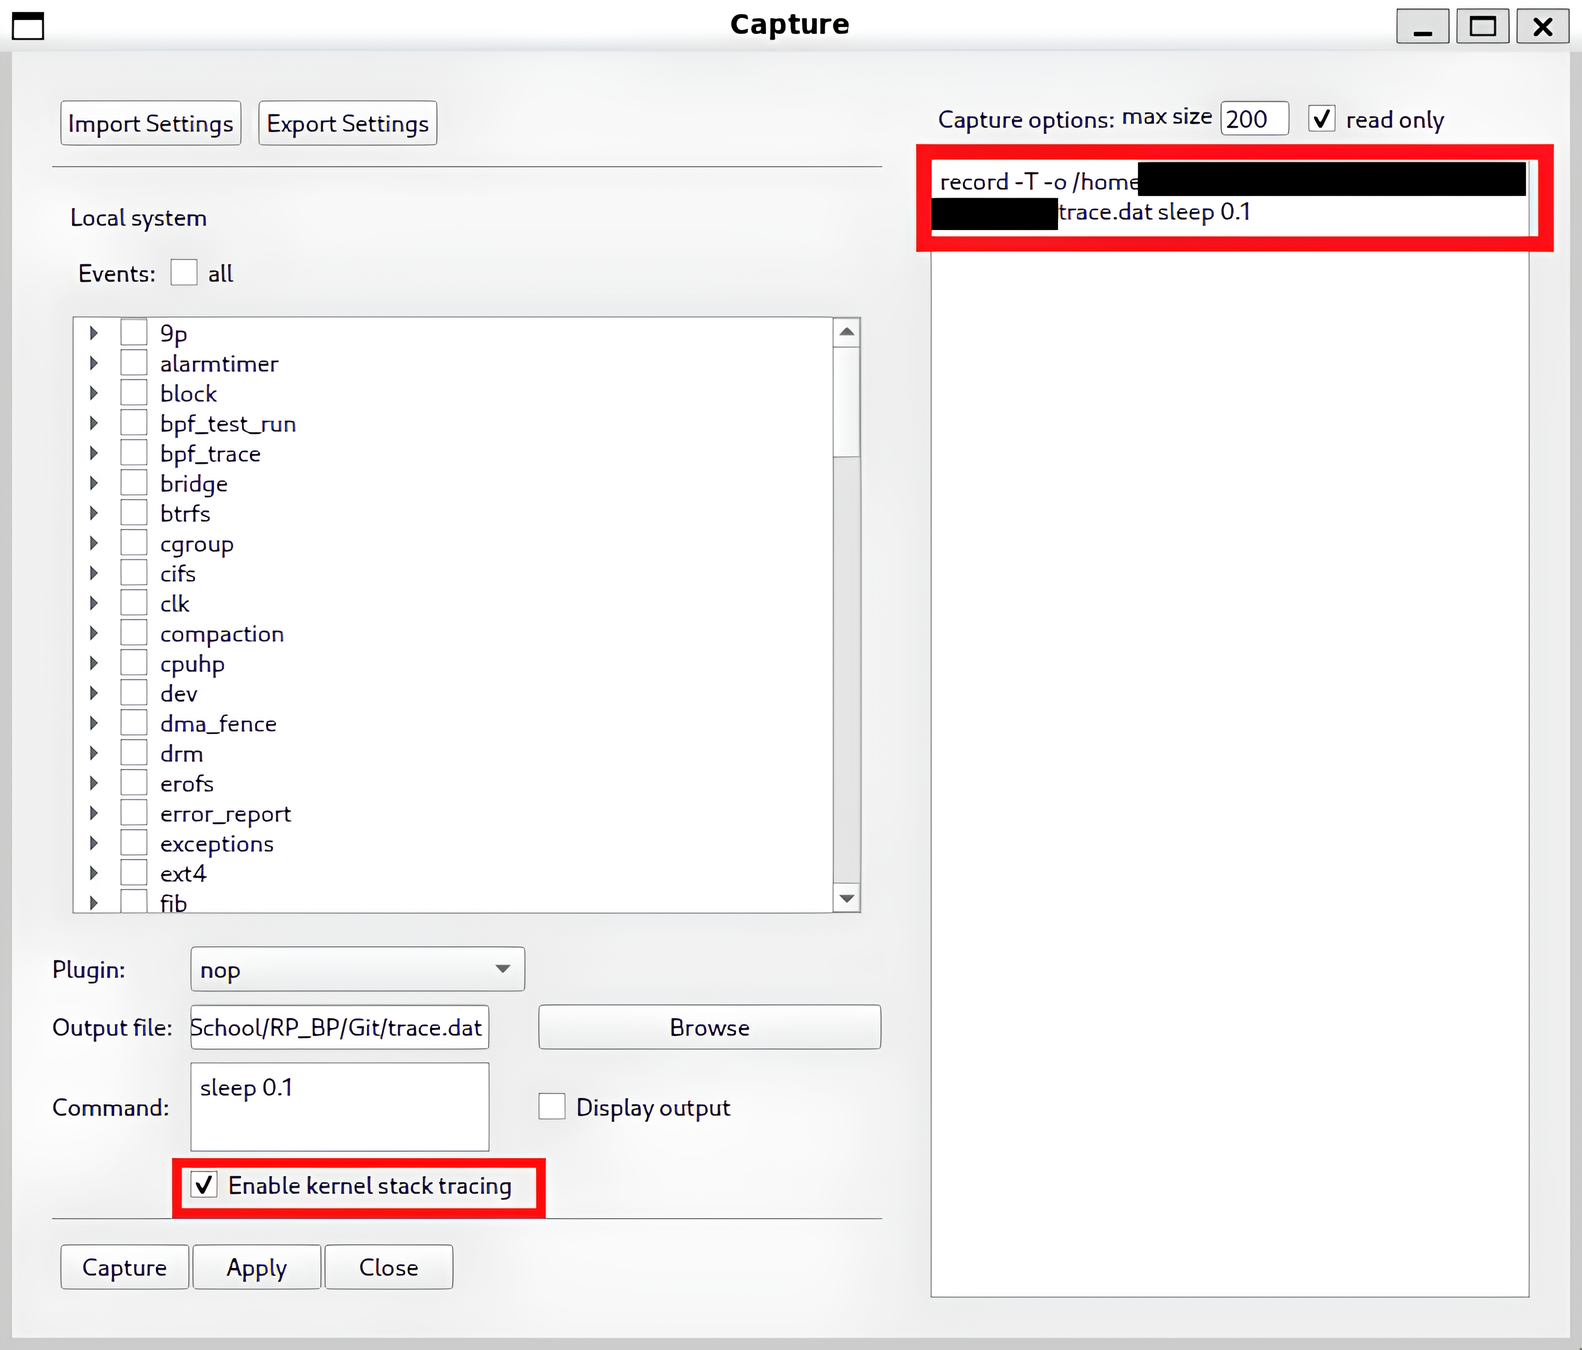
\includegraphics[width=140mm]{img/Modifikace/modif-record-kstack}
    \caption{Zvýraznění změn této modifikace viditelných v GUI}
    \label{obr01:record-kstack}
\end{figure}

\section{Rozšíření}

Ne každá událost může mít zajímavý zásobník. Možnost zachytávat pouze po některých událostech by zde pomohla. Nicméně to je spíše rozšíření pro trace-cmd. KernelShark by mohl umět ignorovat záznamy zásobníku jádra, pokud navazují na nějakou událost, po které nás zásobník nezajímá. Data budou stále v souboru, ale KernelShark by je nenačetl.

\section{Zhodnocení splnění požadavků}
Jediný vlastní požadavek této modifikace bylo přidání zaškrtávacího tlačítka pro jasnější zapínání sběru zásobníků kernelu. Toto bylo splněno přidáním takového tlačítka do Record okénka a připsání interpretace zaškrtnutí jako dodání argumentu trace-cmd.

Obecné požadavky byly splněny také, GUI prvek byl přidán, kód byl rozšířen. Žádná modifikace existujícího chování se neudála. Tlačítko je ve výchozím stavu nezaškrtnuté a lze jej po zaškrtnutí odškrtnout. Tím jsou obecné požadavky splněny.                   %%% ANALÝZA & VÝVOJ & UŽÍVÁNÍ pro kažou část zvlášť
\chapter{Stacklook}
Tato kapitola se zabývá pluginem pro KernelShark, díky kterému bude jednodušší analyzovat trasovací data, kde se zachytával zásobník kernelu. V kapitole se seznámíme s cíli, analýzou řešení, návrhem a použitím tohoto pluginu.

\section{Cíle}

\begin{itemize}
    \item Nad podporovanými záznamy bude klikatelný objekt - po dvojitém kliknutí se zobrazí vyskakovací okénko.
    \item Tlačítka se budou zobrazovat nad záznamy jak v CPU grafech, tak v grafech procesů.
    \item Ve vyskakovacím okénku se zobrazí záznam zásobníku, název procesu, kterému událost záznamu patří a nějaká bližší informace specifická pro událost, nad kterou bylo tlačítko zobrazeno.
    \item Plugin bude mít konfigurační okénko, kde se bude moci některé chování upravit. Minimální součástí musí být zapínání a vypínání kreslení tlačítek nad podporovanými záznamy, úprava barev tlačítek a nastavování maximálního počtu viditelných záznamů v grafu, při jehož překročení se tlačítka nebudou zobrazovat.
    \item Informační řádek bude schopen zobrazit část zásobníku při přejetí kurzoru myši přes tlačítko. Která část zásobníku se zobrazí bude nastavitelné v konfiguraci pluginu. Jelikož informační řádek nemůže být změněn přes rozhraní pluginů a grafové objekty pluginů nereagují na přejetí myší, toto budou dodatečné modifikace, resp. modifikace \emph{Preview Labels Changeable} a \emph{Mouse Hover Plot Objects}.
    \item Tlačítka mohou být barevná stejně jako je zabarven proces, kterému záznam pod tlačítkem náleží. Získání barev procesů, CPU a streamů není v KernelSharku možné, KernelShark dovoluje barevné tabulky jenom vytvořit nanovo, které ovšem nebudou synchronizovány s tabulkami využívanými KernelSharkem. Zpřístupnění těchto tabulek bude dodatečná modifikace s názvem \emph{Get Colors}.
    \item Je nutné podporovat alespoň události typu sched/sched\_switch a sched/sched\_waking.
    \item Plugin bude možné používat i pro KernelShark bez modifikací vytvořených jako součást této práce.
\end{itemize}

Poslední bod existuje pro případné uživatele, kteří nechtějí používat modifikovaný KernelShark, dokud nejsou modifikace součástí oficiálního vydání. Plugin se tak může využívat i v úplné izolaci od ostatních změn z této práce, což souhlasí s obecnými požadavky na pluginy. Ostatní cíle vychází z kapitoly \emph{Obecná analýza a stanovení požadavků}. Jako samozřejmost se bere technická a uživatelská dokumentace a splnění obecných požadavků na pluginy.

\section{Analýza}
Tato sekce se pokusí zachytit postup, kterým se dostaneme k implementaci řešení. Jedná se o techničtější analýzu než analýza z kapitoly \emph{Obecná analýza a stanovení požadavků}.

Zamysleme se nyní nad tím, jak bychom vytvořili plugin pro KernelShark s našimi cíli. Nejlepším začátkem by bylo nechat se inspirovat oficálními pluginy, od nich se lze naučit, jak plugin propojit s KernelSharkem. Oficiální pluginy definují hlavičkový soubor v jazyce C, kde se definuje kontext pluginu. Tento kontext je pak struktura s globálně přístupnými daty pro plugin. S kontextem se i deklarují kontextové funkce ovládající jeho inicializaci a destrukci přes KernelSharkem definované makro. Krom toho se zde deklarují i další globálně přístupné prvky, které nevyžadují funkcionality C++. Tento hlavičkový soubor může své části implementovat jak C kódu, tak v C++ kódu. Oficiální pluginy mají v C napsanou hlavně definici kontextových funkcí, registraci handlerů pro různé události během načítání trasovacích dat, registrace handlerů na kreslení do grafu, inicializaci dat pro textový font a inicializaci ukazatelů na hlavní okno. Handlery jsou buď implementovány v C++, nebo, hlavně u jednoduchých handlerů událostí, ještě v implementačním C souboru. Kód napsaný v C je tedy většinou použit na inicializaci pluginu a další části, většinou s komplikovanější business logikou, jsou implementovány v C++.

Postup oficiálních pluginů je dobrý, využijeme jej tedy též. Stacklook ovšem bude vyžadovat více C++ kódu. Jednotlivé soubory pak budou sloužit jednotlivým modulům Stacklooku, například modul konfigurace bude obsahovat datovou struktury či datové struktury, které konfiguraci tvoří. Pokud možno, hlavičkové soubory by pak měly reprezentovat každý jeden z modulů. Podobné postupy jsou hojně využívány, hlavně při dekompozicích souboru s kódem, který obsahuje vícero modulů najednou.

Z našich cílů lze celkem přímo vymezit moduly, ze kterých se bude plugin skládat: \emph{Propojující modul}, \emph{Konfigurace}, \emph{Tlačítka}, \emph{Detailní pohledy}.

Propojující modul máme zčásti navržen díky oficiálním pluginům. V \uv{C části} (napsaná v jazyce C) nastavíme textový font používaný v pluginu, vybereme podporované události při načítání dat a registrujeme handlery. V \uv{C části} zároveň inicializujeme pluginový kontext. Tato část bude mít za úkol tento kontext i správně odstranit. V \uv{C++ části} definujeme handlery pro kreslení a přístup k hlavnímu oknu. Kreslící handler bude vyžadovat funkci na vytvoření tlačítek, tedy zde se propojí tlačítkový modul. Funkce vytvoření tlačítek bude potřebovat data pro barvu tlačítek, ta je v konfiguraci, takže se zde objeví i konfigurační modul. Tento modul bude také obsahovat podporované události a bude je sbírat do dat v kontextu pluginu.

Konfigurace bude rozdělená mezi GUI okno a datovou strukturu s konfiguračními daty, tzv. konfigurační objekt. Konfigurační objekt samotný implementujeme jako singleton. Důvodem je nutnost znát konfiguraci v různých částech programu a že konfigurace musí být vždy pouze jedna, což právě singleton splňuje. Prvky z cíle o konfiguraci můžeme jednoduše uložit jako čísla, pravdivostní hodnoty, textové řetězce a datovou strukturu pro barvy od KernelSharku. Aby bylo možné konfiguraci měnit pouze skrze konfigurační okno, tyto prvky schováme pomocí modifikátorů viditelnosti. Konfigurační objekt pak využije C++ mechanismus \uv{zpřátelení} přes klíčové slovo \texttt{friend} a označí konfigurační okno za svého přítele. Konfigurace pluginů KernelSharku nejsou persistentní, tak dodáme i nějaké výchozí hodnoty. Kvůli zobrazování zásobníku v informačním řádku, přidáme ke každému nastavení specifickému pro událost i offset od vrchu zásobníku. Tak budeme moci stanovit oblast zásobníku, ve které se většinou nachází ty nejzajímavější části zásobníku pro danou událost.

Konfigurační okno využije framework Qt (specificky Qt6), stejně jako ostatní grafické prvky KernelSharku. Na barevná nastavení vytvoříme tlačítko, které na kliknutí vyvolá nějaké okno na výběr barvy, například výchozí barevný dialog od Qt. Pro pohodlí uživatele i někde blízko tlačítka výběru barvy zobrazíme i aktuálně použitou barvu. Nastavení maximálního počtu viditelných záznamů lze reprezentovat jako spinbox. Konfigurace pro specifické události, tj. zdali nad danými událostmi zobrazovat tlačítka nebo offset použitý při zobrazování části zásobníku v informačním řádku, lze reprezentovat pomocí zaškrtávacího tlačítka a dalšího spinboxu. Mimo požadavky navíc dodáme zaškrtávací tlačítko pro barvení tlačítek barvami jejich procesů.

Modul tlačítek se bude hlavně skládat z třídy pro tlačítka. Ta by měla být v grafu jasně viditelná a ihned rozpoznatelná uživatelem. Tvar tlačítek by měl nějak ukazovat, kterému záznamu patří. Zde je několik možností a tvarů na výběr, nicméně nejjednodušším tvarem bude trojúhelník. Jeden z vrcholů bude směřovat dolů, ostatní dva vrcholy budou nad tímto vrcholem. Rozpoznatelnost těchto tlačítek nakonec zajistíme přidáním nápisu \texttt{STACK} do každého z nich. Reakci na dvojité kliknutí a přejetí kurzorem myši implementujeme jako to dělají ostatní tvary definované KernelSharkem. U přejetí využijeme naše modifikaci na reakci na přejetí kurzorem myši a modifikaci na změnu informačního řádku, přesně jak říká jeden z cílů. Speciálně pro sched\_switch budou tlačítka ještě obsahovat jedno písmeno symbolizující předchozí stav procesu před přepnutím. Takto nebude nutné se podívat do detailního pohledu, bude stačit se dívat do grafu. Nicméně uživatel bude muset znát zkratky pro možné předchozí stavy. Ty jsou součástí dokumentace Linuxu. [TODO: Sem se asi hodí zdroj.] Barva tlačítek bude určena hodnotami v konfiguračním objektu. Dodáme i možnost používat barvy procesů jako barvy tlačítek, to nám zajistí modifikace \emph{Get Colors}. Aby nemohlo více tlačítek splývat díky stejné barvě, tlačítka budou mít obrys, jehož barva bude také dána konfigurací a bude oddělená od (vnitřní) barvy tlačítka.

Modul detailních pohledů bude hlavně obsahovat třídu pro okna těchto pohledů. V okně pak zobrazíme záznam zásobníku ve formě seznamu. Tento formát se hodí na jednoduché zvýraznění položky jedním kliknutím. Dodáme ale i možnost si data zobrazit jako prostý text - tento formát je naopak lepší když se kopírují data po jných částech než po položkách. Na vrchol zásobníku dodáme značku \texttt{top}, aby bylo jasné, kde se vrch zásobníku nachází. Jeden z cílů nám ještě udává nutnost zobrazit název procesu a nějaké bližší informace o události. Pro sched\_switch zde můžeme udat přechozí stav procesu před přepnutím, například zdali byl proces již ve stavu zombie, nebo zdali začal čekat na nějaká data a nebo zdali prostě běžel a byl preemptivně přepnut. Předchozí stav zapíšeme jak zkratkou, tak celým názvem (například \uv{S - sleep}, nebo \uv{Z - zombie}). Pro sched\_waking pouze napíšeme, že byl proces probuzen. Nakonec se zamyslíme nad tím, jak dlouho budou okna žít a kolik jich může být najednou pro jednu událost. Naše pohledová okna můžeme vytvořit jako podřízená oknu hlavnímu, tedy pokud je ukončeno hlavní okno, budou ukončena i jeho podřízená okna. Toto zajistí Qt framework. Počet oken pro jednu událost nebudeme omezovat, nic se tím nerozbije a implementace bude jednodušší. Tato rozhodnutí by měla mít ten efekt, že uživatel bude schopen stream, nazvěme jej A, pak bude schopen začít zkoumat stream jiný, nazvěme tento B. Okna otevřená ve streamu A zůstanou otevřená i po přepnutí do streamu B, do té doby dokud je uživatel sám nezavře, nebo dokud uživatel nezavře hlavní okno. Lze tak porovnávat zásobníky z různých běhů trasování.

Na získání informací o předchozím stavu ještě dodáme mini-modul \emph{Předchozí stavy}. Nutně bude muset být schopen vytáhnout data o předchozím stavu ze záznamu události přepnutí v KernelSharku. Tato data pak bud muset umět dodat pluginu buď jako zkratka pro typ stavu (tlačítka a detailní pohledy), nebo jako celý název (detailní pohledy).

Postupujme dále, podívejme se na informační řádek. Informační řádek nabízí pouze pět míst pro text. Pokud bychom museli zobrazovat konec zásobníku, nebo i prvky za koncem (například kvůli vysokému offsetu v konfiguraci), v informačním řádku pak vyznačíme, že jsme na konci zásobníku a místa, kde by byly prvky za koncem označíme nějakou čárou, třeba mínusem. Pokud ale zobrazujeme oblast zásobníku a za ní zásobník pokračuje, označíme toto třemi tečkami v posledním místě pro text v informačním řádku. Nakonec, pro jasnou identifikaci procesu z jehož záznamu zásobníku čerpáme bude první místo v informačním řádku obsazeno názvem tohoto procesu. Prvky v informačním řádku tedy budou vždy v následujícím pořadí:
\begin{itemize}
  \item Název procesu
  \item Věc na zásobníku na offsetu X od vrcholu zásobníku, nebo \texttt{-}
  \item Věc na offsetu X+1, nebo \texttt{-}
  \item Věc na offsetu X+2, nebo \texttt{-}
  \item \texttt{...}, nebo \texttt{(End of stack)}
\end{itemize}
Informační řádek bude vždy schopen zobrazit nejvýše tři prvky ze zásobníku.

Nakonec se zamyslíme, jak získat data záznamů zásobníku kernelu. Tlačítka jsou nad záznamy, po kterých následuje záznam zásobníku. Tyto záznamy se vždy vytvoří na stejném CPU jako událost jim předcházející. Během načítání dat ale ještě nemáme události seřazené, ovšem při prvním kreslení už ano. Navíc neplatí, že všechny soubory trasovacích dat musí obsahovat záznamy zásobníku, lze systém trasovat i bez sbírání zásobníku. V tom přípaě nemá smysl, aby plugin cokoli kreslil. Do kontextu pluginu dodáme dvě proměnné, jednu jako indikátor \uv{hledali jsme záznam trasování zásobníku kernelu} a druhou jako \uv{záznam trasování zásobníku existuje}, přičemž obě začnou na pravdivostní hodnotě \uv{nepravda}. Při prvním kreslení prohledáme následníky všech záznamů námi podporovaných událostí. Pokud alespoň jeden záznam má za následníka záznam zásobníku, nastavíme druhou proměnnou v kontextu na \uv{pravda}. Ukazatel na tento záznam si pak poznamenáme i u záznamu předcházející události. Po prohledání všech podporovaných záznamů nastavíme i první proměnnou na \uv{pravdu}. Tak si zajistíme jediný chod při hledání těchto dat. Ačkoliv prohledávání může trvat dlouho, stane se tak pouze jednou a časová cena prohledávání tak není příliš výrazná.

\subsection*{Plugin pro nemodifikovaný KernelShark}

Každá část implementace využívající nějakou z našich modifikací bude obalena podmínkovým \texttt{ifndef} makrem s názvem \texttt{\_UNMODIFIED\_KSHARK}. Toto makro bude aktivováno pokud uživatel při sestavování tuto proměnnou definuje argumentem pro CMake, více v uživatelské dokumentaci v sekci o instalaci. Pokud je makro definováno, pak zvolí alternativní implementaci z \texttt{else} větve, která nevyužívá žádnou z modifikací; jinak kód nebude součástí kompilace.

\section{Vývojová dokumentace}

\subsection*{Dokumentace pluginu}
Dokumentace je napsána pro nástroj Doxygen. Dokumentovala se každá funkce i proměnná, nicméně vygenerovaná dokumentace obsahuje jenom prvky veřejné, pro skutečné implementační detaily je tedy doporučeno se podívat do zdrojového kódu. Dokumentace navíc obsahuje hlavní stránku a stránku s nástinem návrhu.

\subsection*{Struktura projektového adresáře}

Adresář pluginu obsahuje další adresáře. Adresář \uv{src} pro zdrojový kód a adresář \uv{doc} pro dokumentaci uživatelskou a dokumentaci technickou. Očekává se, že na této úrovni jsou i adresáře pro sestavení. Na stejné úrovni bude žije i README, soubor s licencí a nejvyšší CMakeLists.txt. V těchto CMake instrukcích se nastaví proměnné sestavení, například typ sestavení, a případně se zavolá generace dokumentace. CMake instrukce zodpovědné za vytvoření binárního souboru dáme do adresáře se zdrojovým kódem, stejně jako to dělá KernelShark.

\subsection*{Přehled modulů pluginu}

\begin{itemize}
    \item \emph{Propojující modul} - Modul s kódem propojujícím KernelShark a plugin. Obsahem je hlavně kontext pluginu, funkce kontextu, handlery a implementačně pomocné funkce. Součástí tohoto modulu je část s C kódem a implementační část v C++ prvků z hlavičkového C souboru,. Právě v \uv{C++ části} (napsaná v C++) se ostatní moduly budou propojovat; zároveň tato část bude ukládat některá globální data s C++ typy. Soubory modulu jsou \emph{stacklook.h/c} a \emph{Stacklook.cpp}.
    \item \emph{Konfigurace} - Modul se skládá ze dvou tříd, konfigurační objekt a konfigurační okénko. Konfigurační objekt obsahuje konfigurační data, která plugin zrovna využívá a je navržen jako singleton. Konfigurační okénko představuje GUI element, kterým se data v konfiguračním objektu manipulují. Soubory modulu jsou \emph{SlConfig.hpp/cpp}.
    \item \emph{Tlačítka} - Tlačítka jsou vykreslována v grafu nad záznamy podporovaných událostí. Dokáží reagovat na dvojité kliknutí myši, čímž vyvolají detailní pohled na zaznamenaný zásobník, nebo přejetí nad nimi, kdy zobrazí část zásobníku v informačním řádku. Soubory modulu jsou \emph{SlButton.hpp/cpp}.
    \item \emph{Detailní pohledy} - Detailní pohledy jsou grafická okna zobrazující zaznamenaný kernel zásobník, informace o události, která záznamu zásobníku předcházela, a informace o procesu vlastnící tuto událost. Soubory modulu jsou \emph{SlDetailedView.hpp/cpp}.
    \item \emph{Předchozí stavy} - Mini-modul, dodává data tlačítkům a detailním pohledům o stavu procesu před přepnutím kontextu na CPU. Soubory modulu jsou \emph{SlPrevState.hpp/cpp}.
\end{itemize}

\section{Uživatelská dokumentace}

Tato sekce popíše jak instalovat a používat plugin Stacklook v KernelSharku a co od něj během běhu očekávat, či na co si dát pozor. Obrázek \ref{SlWorking} ukazuje fungující plugin v akci.

\begin{figure}[p]\centering
    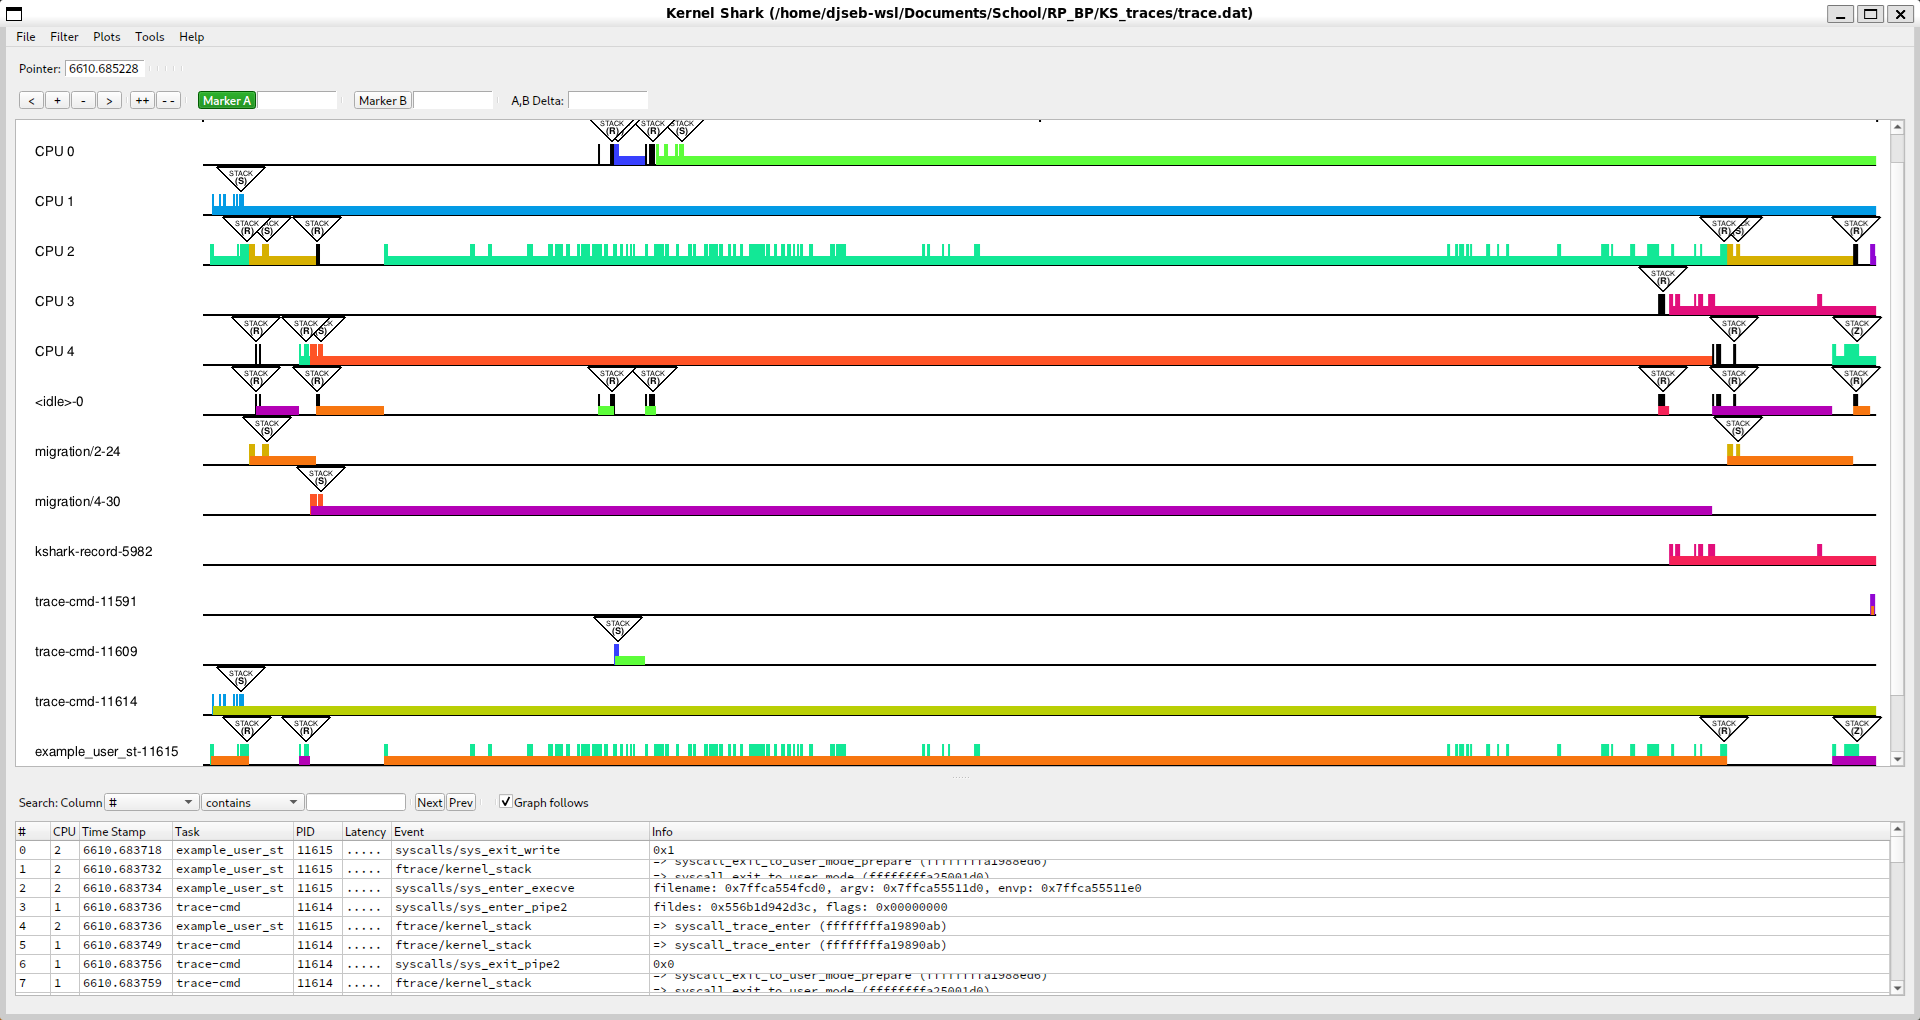
\includegraphics[width=140mm]{img/Stacklook/SlWorking}
    \caption{Fungující Stacklook}
    \label{SlWorking}
\end{figure}

\subsection{Jak sestavit a instalovat Stacklook}

\subsubsection*{Kompatibilita}

\begin{itemize}
  \item CMake verze alespoň 3.1.2.
  \item Pokud chcete plugin využívající modifikovaný KernelShark, pak je nutná verze alespoň 2.4.0-couplebreak. Pokud chcete plugin pro nemodifikovaný KernelShark, pak je nutná verze alespoň 2.3.2.
  \item Závislosti KernelSharku (naleznete v README repozitáře KernelSharku), zejména Qt6.
  \item Doxygen na technickou dokumentaci.
\end{itemize}

\subsubsection{Sestavení a instalace pouze pluginu}

\begin{enumerate}
  \item V terminálu nastavte pracovní adresář na složku \texttt{build} (pokud ještě neexistuje, pak ji nejlépe vytvořte v kořenovém adresáři projektu).
  \item Spusťte příkaz \texttt{cmake ..}. Pokud hlavní soubor \texttt{CMakeLists.txt} není v nadřazené složce, předejte programu CMake platnou cestu k němu.
    \begin{itemize}
      \item Používáte-li verzi KernelSharku bez modifikací, přidejte do příkazu argument \texttt{-D\_UNMODIFIED\_KSHARK}.
      Sestavení pro nemodifikovaný KernelShark odstraňuje tyto funkce:
      \begin{itemize}
        \item Tlačítka mohou být stejné barvy, jako procesy, jimž patří záznamy s tlačítky.
        \item Přejetí myši zobrazí část zásobníku v informačním řádku KernelSharku.
      \end{itemize}
      \item Pokud chcete generovat dokumentaci pomocí Doxygenu, přidejte do příkazu argument \texttt{-D\_DOXYGEN\_DOC=1}.
      \item Výchozí typ sestavení je \texttt{RelWithDebInfo}. Chcete-li ho změnit (např. na \texttt{Release}), použijte argument \texttt{-DCMAKE\_BUILD\_TYPE=Release}.
      \item Pokud se soubory Qt6 nenacházejí ve \texttt{/usr/include/qt6}, použijte argument \texttt{-D\_QT6\_INCLUDE\_DIR=[PATH]}, kde \texttt{[PATH]} nahradíte cestou k souborům Qt6.
        \begin{itemize}
          \item Pokyny pro sestavení předpokládají, že zadaný adresář má stejnou vnitřní strukturu jako výchozí možnost (tj. obsahuje složky QtCore, QtWidgets apod.).
        \end{itemize}
      \item Pokud se zdrojové soubory KernelSharku nenachází v \texttt{../KS\_fork/src}, použijte argument \texttt{-D\_KS\_INCLUDE\_DIR=[PATH]}, kde \texttt{[PATH]} nahradíte cestou ke zdrojovým souborům KernelSharku.
      \item Pokud se sdílené knihovny KernelSharku (\texttt{.so} soubory) nenachází ve \texttt{/usr/local/lib64}, použijte argument \texttt{-D\_KS\_SHARED\_LIBS\_DIR=[PATH]}, kde \texttt{[PATH]} nahradíte cestou k sdíleným knihovnám KernelSharku.
    \end{itemize}
  \item Ve složce \texttt{build} spusťte příkaz \texttt{make}.
    \begin{itemize}
      \item Pokud je třeba sestavit jen část pluginu, napříkla pouze dokumentaci, můžete vybrat konkrétní cíl.
      \item Pouhé spuštění \texttt{make} vytvoří: \emph{plugin} (cíl \texttt{stacklook}), \emph{symlink} na sdílený objekt pluginu (cíl \texttt{stacklook\_symlink}) a případně \emph{Doxygen dokumentaci} (cíl \texttt{docs}), pokud tak bylo specifikováno v předchozím kroku.
    \end{itemize}
  \item (\emph{Instalace}): Nahrajte plugin do KernelSharku, buď přes GUI, nebo při spouštění přes CLI s argumentem \texttt{-p} a cestou k symlinku nebo přímo k sdílenému objektu.
    \begin{itemize}
      \item \emph{DŮLEŽITÉ}: Vždy nainstalujte/nahrajte plugin před načtením relace, ve které byl aktivní! Jinak může dojít k neúplnému načtení konfiguračního rozhraní nebo k pádu celého programu.
    \end{itemize}
\end{enumerate}

K odstranění vytvořených binárních souborů použijte \texttt{make clean}.

\subsubsection{Sestavení a instalace pomocí KernelSharku}

\begin{enumerate}
  \item Ujistěte se, že všechny zdrojové soubory (\texttt{.c}, \texttt{.cpp}, \texttt{.h}) Stacklooku se nacházejí ve složce \texttt{src/plugins} v adresáři projektu KernelShark.
  \item Zkontrolujte, že soubor \texttt{CMakeLists.txt} v této podsložce obsahuje instrukce pro sestavení pluginu (inspirovat se můžete podle jiných pluginů pro GUI). Pokud chcete sestavovat pro nemodifikovaný KernelShark, upravte tomu odpovídajícím způsobem build skript.
  \item Sestavte KernelShark (pluginy se sestavují automaticky). Lze sestavit i pouze plugin, pokud jste již předtím vytvořili instrukce sestavení.
  \item (\emph{Instalace}): Spusťte KernelShark. Pluginy sestavené tímto způsobem se načítají automaticky. Pokud by se z nějakého důvodu nenačetly, najděte sdílený objekt stejně jako u ostatních oficiálních pluginů, opět buď přes GUI, nebo přes CLI.
\end{enumerate}

\subsubsection{VAROVÁNÍ - načítání více verzí pluginu}

Máte-li dvě nebo více sestavených verzí pluginu, \emph{NE}načítejte je současně do KernelSharku. Pokud to uděláte, \emph{DOJDE K PÁDU PROGRAMU}. Používejte vždy jen jednu z verzí, \emph{NIKDY OBOJE NAJEDNOU}.

\subsection{Jak zapnout/vypnout Stacklook}

Zapnutí pluginu je velmi jednoduché. Stačí spustit KernelShark a přejít na položku v panelu nástrojů \texttt{Tools > Manage Plotting plugins}. Pokud byl plugin načten přes příkazový řádek, zobrazí se v seznamu pluginů jako zaškrtnuté políčko se svým názvem. Pokud ne, lze plugin dohledat pomocí tlačítka \texttt{Tools > Add plugin} - stačí nalézt symlink, ale je možné vybrat i samotný soubor sdíleného objektu. Jak je vidět, plugin využívá standardní mechanismus načítání pluginů v KernelSharku. Obrázek~\ref{SlManagePlottingPlugins} ukazuje GUI pro zapínání a vypínání pluginů.

\begin{figure}[p]\centering
    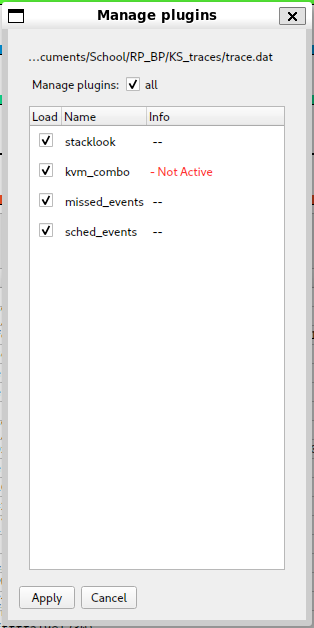
\includegraphics[height=140mm]{img/Stacklook/SlManagePlottingPlugins}
    \caption{Okénko se správou pluginů}
    \label{SlManagePlottingPlugins}
\end{figure}

\subsection{Jak používat Stacklook}

\subsubsection{Konfigurace}

Konfigurace pluginu může být provedena kdykoliv, i před načtením jakýchkoliv trasovacích dat. Pro otevření konfiguračního okna (viz obrázek~\ref{SlConfigWindow}) stačí v hlavním okně zvolit \texttt{Tools > Stacklook Configuration}. Vždy může být otevřeno jen jedno konfigurační okno.

\begin{figure}[p]\centering
    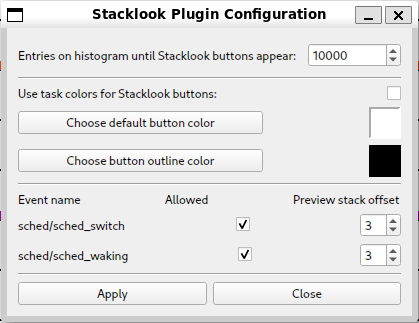
\includegraphics[width=140mm]{img/Stacklook/SlConfigWindow}
    \caption{Konfigurační okno Stacklooku pro modifikovaný KernelShark}
    \label{SlConfigWindow}
\end{figure}

Používáte-li verzi pluginu pro nemodifikovaný KernelShark, bude v konfiguračním okně chybět zaškrtávací políčko pro barvení tlačítek barvami procesů a nastavení offsetu, použitého při zobrazování prvků zásobníku v informačním řádku, viz obrázek~\ref{SlUnmodifiedKsharkConfigWindow}.

\begin{figure}[p]\centering
    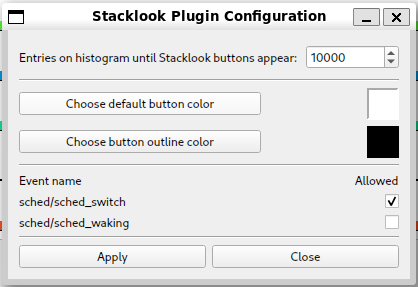
\includegraphics[width=140mm]{img/Stacklook/SlUnmodifiedKsharkConfigWindow}
    \caption{Konfigurační okno Stacklooku pro nemodifikovaný KernelShark}
    \label{SlUnmodifiedKsharkConfigWindow}
\end{figure}

Nyní si popíšeme jednotlivé možnosti konfigurace a jak je ovládat. Seřazeno shora dolů:
\begin{itemize}
  \item \emph{Limit záznamů v histogramu} - snížením této hodnoty omezíte, kdy se Stacklook aktivuje. Aktivace nastane pouze tehdy, pokud je viditelný počet záznamů menší nebo roven této hodnotě. Čím nižší číslo, tím větší přiblížení je třeba k aktivaci Stacklooku. Minimální hodnota je 0, maximální 1~000~000~000 (jedna miliarda), tato horní mez však bude pravděpodobně zřídka využita. Výchozí hodnota je 10~000 (deset tisíc).
  
  \item \emph{Použít barvy procesů pro tlačítka Stacklooku} - zaškrtnutím tohoto políčka (pokud je k dispozici) bude výplň tlačítek Stacklooku zabarvena barvou procesu, ke kterému patřila událost, pro niž Stacklook našel záznam zásobníku. Pokud políčko necháte nezaškrtnuté, použijí se barvy v konfiguraci Stacklooku (výchozí barvy na obrázku~\ref{SlDefaultColors}). Tato volba je ve výchozím stavu vypnutá.
  
  \begin{figure}[p]\centering
      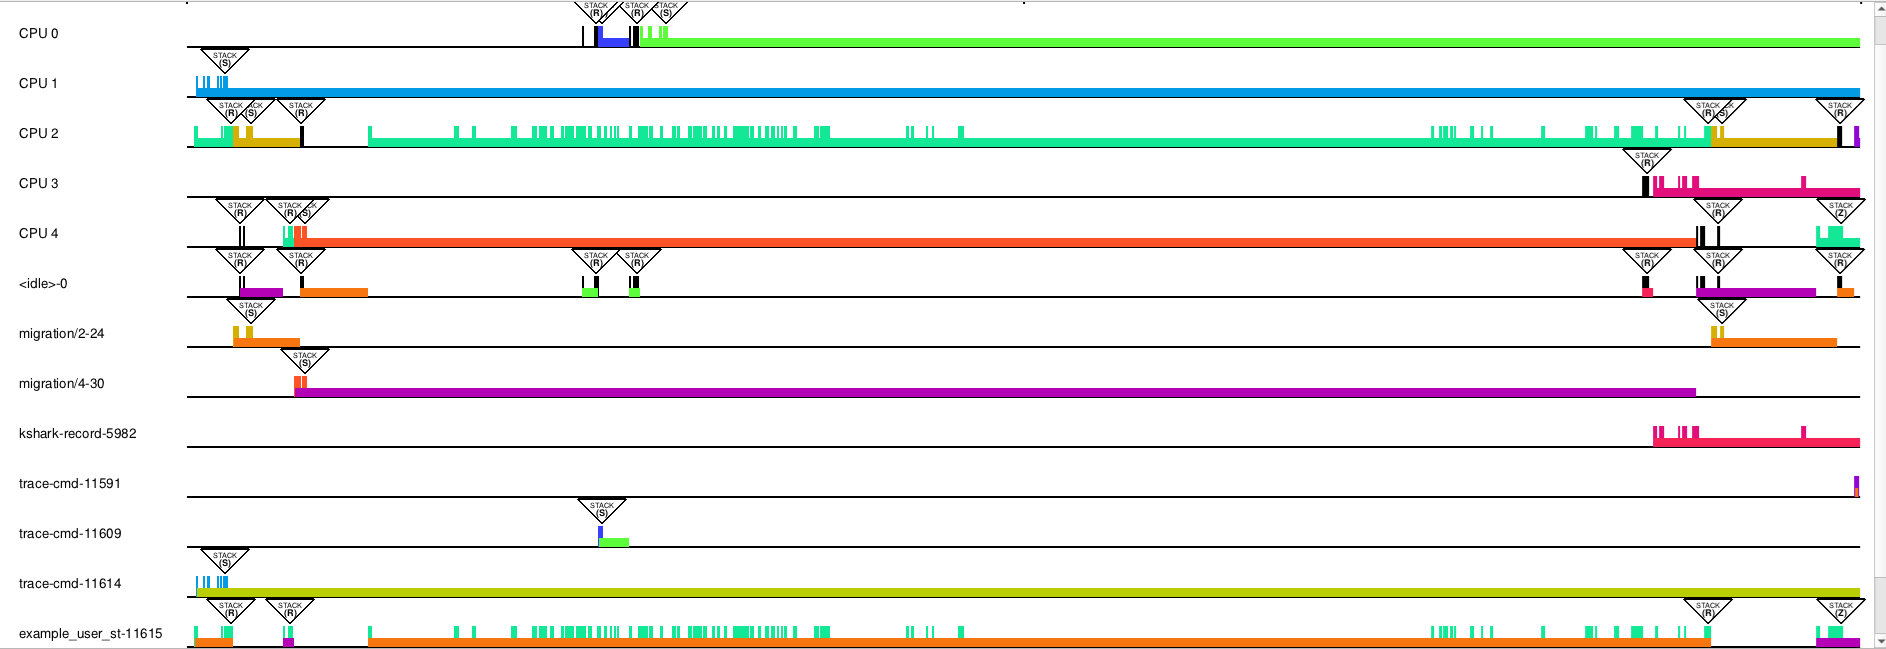
\includegraphics[width=140mm]{img/Stacklook/SlDefaultColors}
      \caption{Tlačítka s výchozími barvami}
      \label{SlDefaultColors}
  \end{figure}
  
  \begin{figure}[p]\centering
      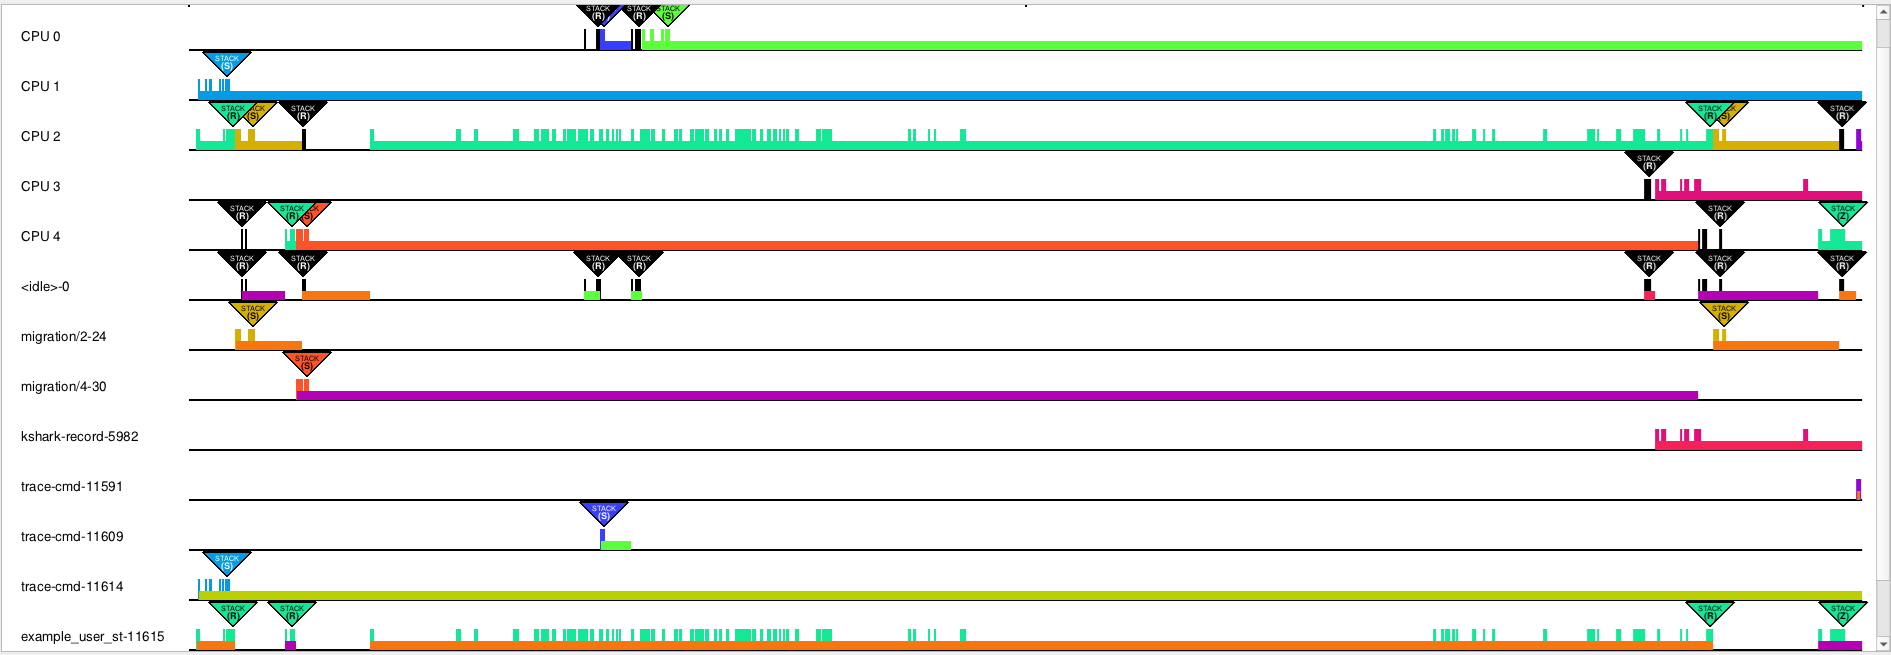
\includegraphics[width=140mm]{img/Stacklook/SlTaskColors}
      \caption{Tlačítka využívající barvy procesů}
      \label{SlTaskColors}
  \end{figure}

  \item \emph{Barvy tlačítek Stacklooku a jejich obrysů} - tlačítka \texttt{Choose} otevřou dialog pro výběr barev, kde lze nastavit barvu výplně tlačítka nebo jeho obrys. Tato nastavení mají účinek pouze tehdy, pokud není dostupná nebo není aktivní volba barev podle procesů. Vedle tlačítek je zobrazen náhled aktuálně vybraných barev. Výchozí nastavení je bílá výplň a černý obrys. Příklad jiných barev si lze prohlédnout na obrázku~\ref{SlCustomDefaultColors}.
  
  \begin{figure}[p]\centering
      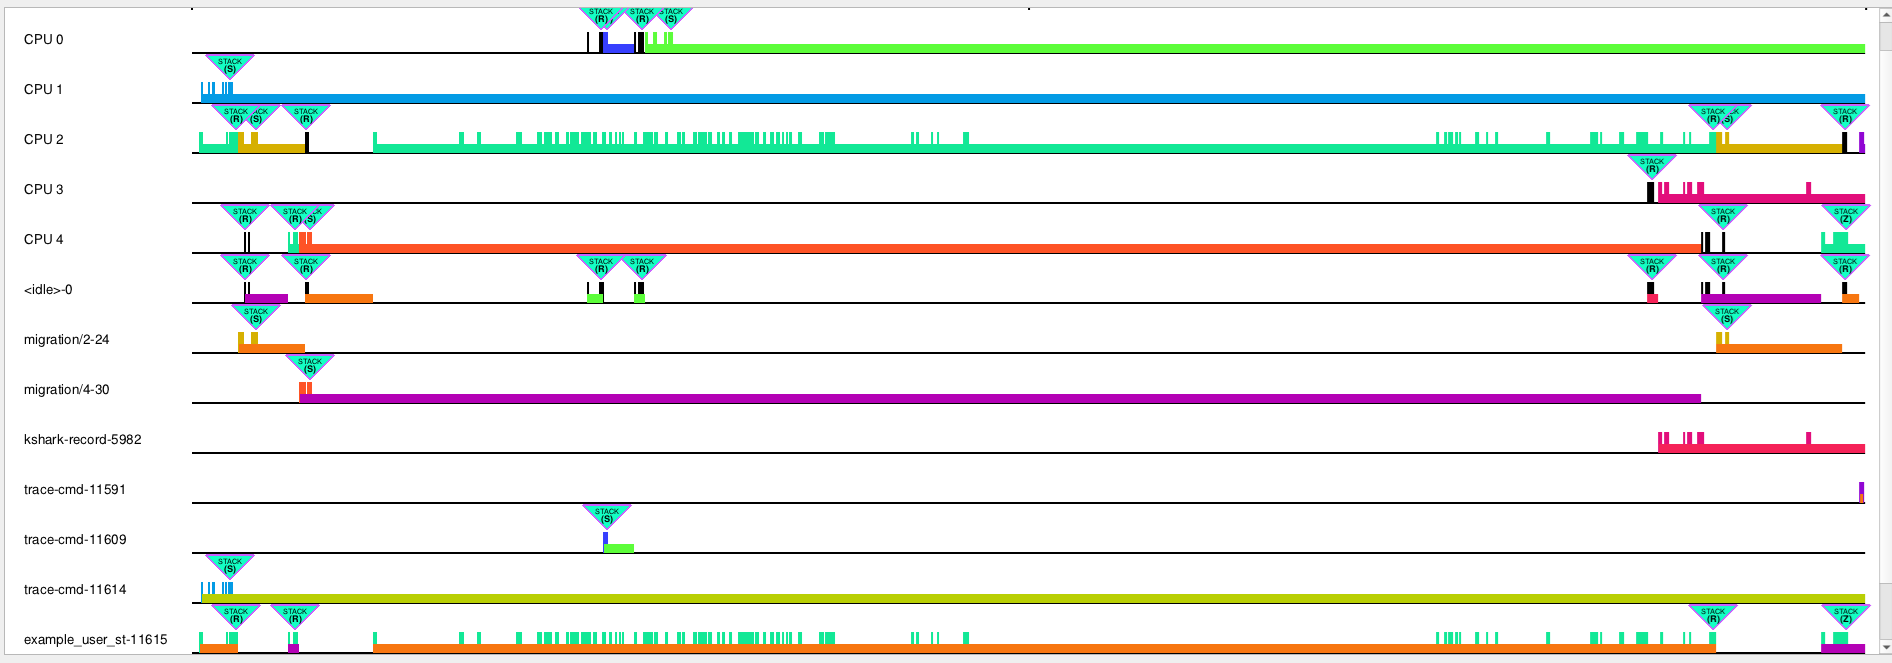
\includegraphics[width=140mm]{img/Stacklook/SlCustomDefaultColors}
      \caption{Tlačítka s konfigurovanými barvami}
      \label{SlCustomDefaultColors}
  \end{figure}

  \item \emph{Nastavení pro jednotlivé události} - Každá událost má své vlastní zaškrtávací políčko, kterým lze Stacklook zapnout nebo vypnout pro daný typ záznamu, a (pokud je k dispozici) číselník s offsetem do zásobníku kernelu, který slouží k určení \uv{nejzajímavější} oblasti v zásobníku pro danou událost. Maximální hodnota offsetu je 100~000~000 (sto milionů), minimální 0. I zde je nepravděpodobné, že by bylo třeba využít maximální hodnotu. Ve výchozím stavu jsou všechny události povoleny (zaškrtnuty) a offset je nastaven na 3.

  \begin{itemize}
    \item Připomenutí - číselník offsetu se nezobrazí, pokud je použit nemodifikovaný KernelShark.
  \end{itemize}
\end{itemize}

Tlačítko \texttt{Apply} uloží provedené změny a zavře konfigurační okno - pokud toto tlačítko nebude stisknuto, změny se neprojeví. V ovládacích prvcích konfiguračního okna se zobrazují pouze aktuálně platné hodnoty konfigurace, konfigurační okno si po zavření neaplikované změny nepamatuje. Tlačítko \texttt{Close} i tlačítko s křížkem v pravém horním rohu okna změny zahodí a okno zavřou.

U Stacklooku nelze konfigurovat:
\begin{itemize}
\item Podporované události - plugin momentálně podporuje pouze události sched/sched\_switch a sched/sched\_waking.
\item Text v oknech detailních pohledů.
\item Text tlačítek.
\item Velikost tlačítek.
\item Pozice tlačítek.
\end{itemize}

Konfigurace není persistentní. Její momentální stav se nikam neukládá, ani do relací.

\subsubsection{V grafu}

Po načtení (a případné konfiguraci) pluginu přibližte zobrazení tak, aby bylo v grafu viditelných méně záznamů, než je nastavený limit. Nad každým podporovaným záznamem se objeví tlačítko - buď ve výchozí barvě z konfigurace, nebo, pokud používáte upravený KernelShark a máte zapnutou příslušnou část nastavení, bude tlačítko obarveno podle procesu. Používání barev procesů je plně kompatibilní s barevným posuvníkem KernelSharku.

Plugin nezobrazí tlačítka nad nepodporovanými událostmi nebo pokud podporovaná událost nenajde záznam zásobníku, ze kterého by bylo možné čerpat data.

\emph{Pokud používáte modifikovaný KernelShark}, přejeďte kurzorem nad libovolné tlačítko a informační řádek KernelSharku. Obsah řádku se změní a zobrazí:
\begin{itemize}
  \item Název procesu jako první (nejlevější) položku.
  \item Položku v zásobníku kernelu na pozici danou konfigurovaným offsetem od vrcholu zásobníku.
  \item Položku v zásobníku kernelu následující po první.
  \item Položku v zásobníku kernelu následující po druhé.
  \item A nakonec buď tři tečky \texttt{...}, pokud stack obsahuje další položky, nebo zprávu \texttt{(End of stack)}, pokud už žádné další položky nezbývají.
\end{itemize}

Pohleďme na obrázek~\ref{SlMouseHover} s malou ukázkou této funkcionality. Součástí je také okno Stacklooku (o nich více níže) a záznam zásobníku kernelu v hlavním okně v seznamu všech událostí. Vše je takto uspořádáné, aby bylo zřejmé, že položky v informačním řádku skutečně pocházejí ze zásobníku (použitý offset byl výchozí, tedy 3). Červený kruh zvýrazňuje záznam, nad kterým právě kurzor myši přejíždí.

\begin{figure}[p]\centering
    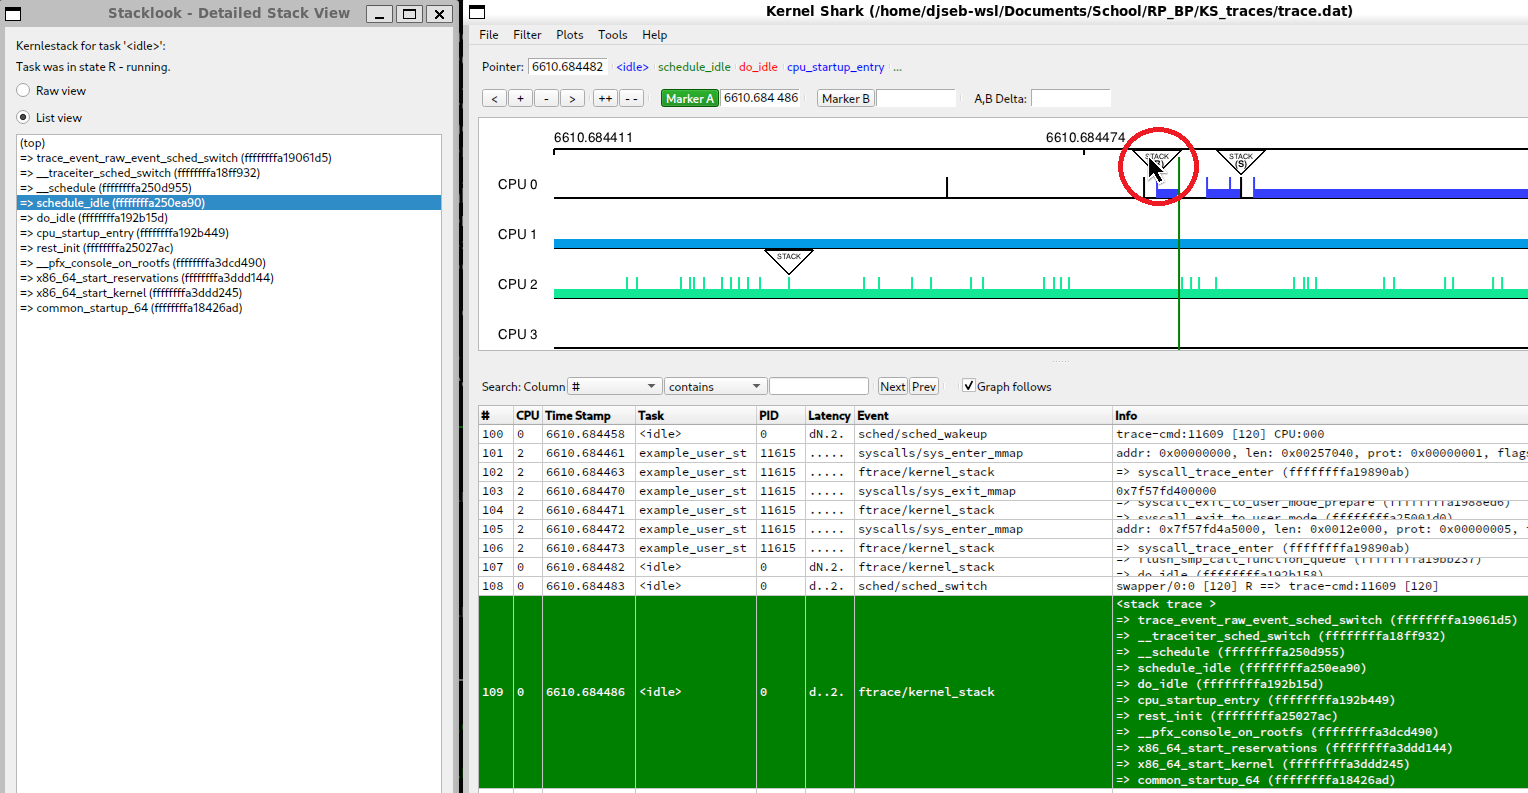
\includegraphics[width=140mm]{img/Stacklook/SlMouseHover}
    \caption{Reakce tlačítek na přejetí kurzorem myši}
    \label{SlMouseHover}
\end{figure}

Offset lze nastavit i tak vysoko, že se v náhledu zobrazí pouze poslední jedna, dvě nebo tři položky, případně žádná. V takovém případě Stacklook zobrazí pouze mínus a zprávu \texttt{(End of stack)} (viz obrázek~\ref{SlTooBigOffset}).

\begin{figure}[p]\centering
    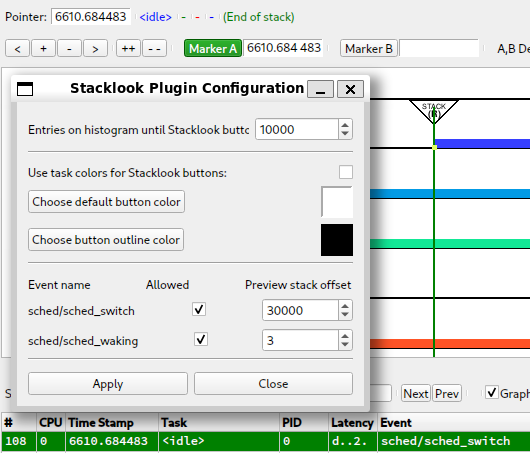
\includegraphics[width=140mm]{img/Stacklook/SlTooBigOffset}
    \caption{Chování informačního řádku při velkém offsetu do zásobníku}
    \label{SlTooBigOffset}
\end{figure}

Po dvojkliku na tlačítko Stacklooku se otevře nové okno detailního pohledu, také nazývané okno Stacklooku. Poku čteme odshora, tak v okně nejprve vidíme, že si prohlížíme zásobník kernelu nějakého procesu. Níže je napsáno, zda byl proces probuzen (zobrazuje se pouze u událostí sched/sched\_waking) nebo o jejím předchozím stavu (pouze u událostí sched/sched\_switch). Následují dvě rádiová tlačítka a zobrazení zásobníku kernelu k dané události. Rádiová tlačítka přepínají mezi různými způsoby zobrazení zásobníku:
\begin{itemize}
  \item Ve výchozím stavu je zobrazení ve formě surového textu, tedy zásobník je pouze řetězec s konci řádků. Toto je užitečné pro zkopírování zásobníku jako jednoho textu nebo pro zvýraznění konkrétní části položky v zásobníku.
  \item Alternativně lze zásobník zobrazit jako seznam, což umožňuje jednodušší a rychlejší (namísto dvojitého kliknutí stačí jedno) zvýraznění jednotlivých položek.
\end{itemize}

Pro jeden záznam může být otevřeno více oken, zároveň může být otevřeno více oken pro různé záznamy, v libovolné kombinaci.

Vše popsáno výše si můžete prohlédnout na obrázku~\ref{SlMultipleWindowsMultipleViewsTwoSameEntires}.

\begin{figure}[p]\centering
    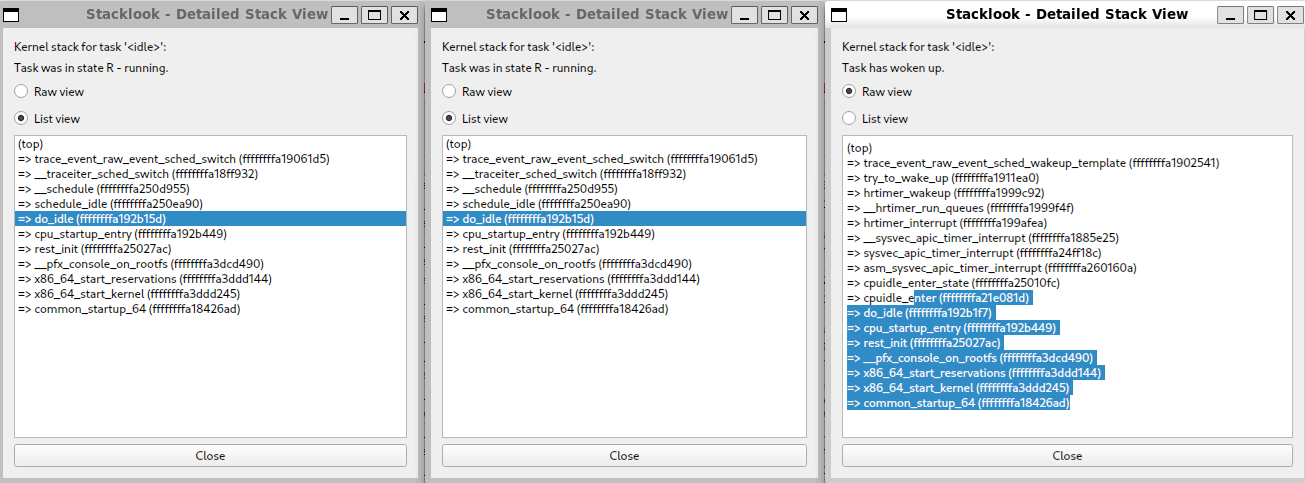
\includegraphics[width=140mm]{img/Stacklook/SlMultipleWindowsMultipleViewsTwoSameEntires}
    \caption{Několik oken detailních pohledů představující svou strukturu}
    \label{SlMultipleWindowsMultipleViewsTwoSameEntires}
\end{figure}

Okno lze zavřít přes tlačítko \texttt{Close} v dolní části okna, nebo pomocí tlačítka s křížkem v hlavičce okna. Všechna okna se zavřou, pokud bude zavřeno hlavní okno KernelSharku. 

\subsection{Bugy a chyby}

Pokud by se tlačítka Stacklook překrývala, bude tlačítko příslušící \emph{starší} události vykresleno nad tlačítkem pro událost \emph{pozdější}, avšak kliknutí nebo najetí myší na překryté tlačítko použije k interakci tlačítko pro \emph{pozdější} událost. Podle autorových znalostí jde o interní chování KernelSharku, které nelze na straně pluginu opravit.

Načtení relace KernelSharku, kde byl Stacklook aktivní, bez předchozího načtení pluginu způsobí \emph{segmentation fault} a \emph{pád programu} při najetí myší na tlačítko Stacklook.

Pokud objevíte další problémy, kontaktujte autora přes e-mail \emph{djsebofficial@gmail.com}.

\subsection{Doporučení}

\begin{itemize}
  \item Vždy načtěte Stacklook před načtením relace. Může to programu ušetřit nepříjemná překvapení.
  \item Neotvírejte stovky a stovky oken Stacklooku, pokud nechcete zbytečně zatížit paměť.
  \item Nedoporučuje se nastavovat příliš vysoký limit záznamů v histogramu v konfiguraci. Jinak by plugin mohl používat příliš mnoho paměti kvůli velkému množství naráz dostupných tlačítek Stacklooku.
  \item I když relace v KernelSharku fungují, jsou trochu nestabilní. Tento plugin se snaží jejich vnitřní logiku nenarušovat, ale varuje, že pokud plugin není načten předem, mohou nastat neočekávané problémy. Například načtení relace s aktivním pluginem nepřidá do menu \texttt{Tools} odpovídající položku pro vyvolání konfiguračního okna.
\end{itemize}

\section{Rozšíření}

Plugin lze rozšířit o další podporované události. Hlavními místy pro tato rozšíření je pak propojující modul, kde se podporované události sbírají a do kontextu se ukládají jejich identifikátory, a mapová konstanta s hodnotami informací specifických pro typ události, která je uvnitř funkci tlačítek, jež vytváří detailní pohledy.                          
\chapter{Couplebreak}
V této kapitole se detailně seznámíme s modifikací pro KernelShark, která je schopna rozdělovat události a vytvářet pro ně záznamy KernelSharku. Tímto se zjemní dělení informací, což některým pluginům dovolí obejít jistá omezení od KernelSharku, kvůli kterým by bylo občas nutné některé pluginy vypnout. Představeny budou cíle, analýza řešení, návrh a použití tohoto vylepšení. Konečnou částí pak bude kritika, ve které modifikaci zhodnotíme a představíme některá rozšíření.

\section{Cíle}
\begin{itemize}
    \item Podporované události dvou procesů dají vzniknout dvěma záznamům - původci a novému umělému záznamu.
    \item Modifikace bude navržena rozšiřitelně o další události.
    \item Nové záznamy budou patřit tomu procesu z páru, který předtím událost nevlastnil.
    \item Nové záznamy budou obsahovat odkaz na záznam s původní událostí.
    \item Nové záznamy budou splňovat rozhraní dotazů na záznamy KernelSharku. To znamená, že bude možné používat \texttt{kshark\_get\_*} funkce jako \texttt{kshark\_get\_pid}, nebo \texttt{kshark\_get\_info} apod.
    \item Nové záznamy bude možné filtrovat jednoduchým filtrem.
    \item Vylepšení bude možno zapnout a vypnout. Toto nastavení bude možné uložit do relací KernelSharku a načíst je z nich.
    \item Součástí vylepšení bude i zajištění kompatibility s pluginem sched\_events.
    \item Podporovány budou alespoň události sched\_switch a sched\_waking.
\end{itemize}

\section{Terminologie}
\begin{itemize}
    \item \emph{Couple/pár} je označení pro dva procesy, které sdílí nějakou událost. Například trasovací událost sched\_waking, kdy nějaký proces rozhodne o probuzení jiného procesu, přirozeně obsahuje dva procesy - probouzejícího a probouzeného. Páry se dají často rozdělit na procesy cílové a počáteční.
    \item \emph{Couplebreak událost} je fiktivní událost vytvořená Couplebreakem. Couplebreak momentálně vytváří pouze události cílové. Modifikace toto vyznačuje v sufixu jména události jako \uv{[target]}. Navíc každá taková událost v KernelSharku obsahuje ve svém jméně prefix \uv{couplebreak/}, podobně jako události plánovače úloh obsahují prefix \uv{sched/}. Couplebreak události mají speciální ID začínající na hodnotě \texttt{-10 000}, které se postupně vždy o 1 snižuje.
    \item \emph{Couplebreak záznam} je záznam vytvářený Couplebreakem pro Couplebreak událost. Významnou vlastností těchto záznamů je, že odkazují na záznam s událostí, kvůli které byla Couplebreak událost vytvořena.
    \item \emph{Origin/počáteční proces} je proces z páru, pro který existuje nějaká událost, se kterou tento proces ovlivní druhý proces z páru.
    \item \emph{Origin event/počáteční událost} je označení pro událost, která náleží počátečnímu procesu.
    \item \emph{Původní událost} je událost, při které se Couplebreak aktivuje a vytvoří Couplebreak událost.
    \item \emph{Target/cílový proces} je proces z páru, pro který existuje nějaká událost, která tento proces nějak ovlivní. 
    \item \emph{Target event/cílová událost} je označení pro událost, která náleží cílovému procesu.
    \item \emph{Vlastník události} je proces, během kterého událost nastala, resp. proces, v jehož grafu se událost objeví.
    \item Termíny \emph{(datový) stream, záznam, událost, relace} jsou převzaty z terminologie KernelSharku.
\end{itemize}

\section{Analýza}
Tato sekce se pokusí zachytit postup, kterým se dostaneme k implementaci řešení. Jedná se o techničtější analýzu než analýza z kapitoly \emph{Obecná analýza a stanovení požadavků}.

\subsection{Vytváření umělých záznamů}
Začněme s jádrem modifikace, rozdělování událostí. Musíme si rozmyslet, kde by bylo možné takovou akci provést. Z logiky fungování programu lze očekávat, že někde se musí události z Trace-cmd přetvořit na záznamy událostí pro KernelShark. Hledáme tedy funkci, která má toto na starosti. Podíváme se na cestu volání programu, když otevřeme nějaký soubor s trasovacími daty. Pak stačí postupovat hlouběji a hlouběji, dokud nenajdeme naši funkci, která nese název \texttt{get\_records}, která vytváří záznamy KernelSharku pro jeden stream. Právě zde KernelShark také vytváří umělé události pro situaci missed\_events, tedy události, které se staly, ale nebyly při trasování zachyceny. Ty KernelShark vytváří před nějakou jinou událostí a tyto umělé události jsou pak umístěny v grafu trasování a seznamu událostí před záznamy událostí, kvůli kterým byly vytvořeny. Navíc má KernelShark jedno hlavní pravidlo pro umělé události - jejich identifikátory musí být záporné. Nyní víme, jak správně vytvářet záznamy pro umělé události a jaká pravidla pro takové události má. Pokud se na funkci \texttt{get\_records} podíváme blíže, najdeme i místo, kde vytvářet umělé události tak, že budou v grafu i seznamu následovat po událostech, které způsobily jejich vznik, tj. původní události. Zde budeme vytvářet cílové události pro sched\_waking a sched\_switch. Druhá z událostí má navíc speciální část ve funkci, z čehož nám plyne i jak vynucovat chování pokud se jedná o nějakou specifickou událost.

Pokračujme tedy návrhem samotných Couplebreak událostí a jejich záznamů v KernelSharku. Identifikátory Couplebreak událostí zvolíme jako negativní hodnoty od hodnoty -10~000 a budou růst po jedné do zápornějších hodnot (tj. budou tvořit sekvenci -10~000, -10~001, -10~002, ...). S identifikátory budou nejspíš chtít pracovat i další části KernelSharku, nebo pluginy, proto je dáme do nového hlavičkového souboru \texttt{libkshark-couplebreak.h}. Identifikátory můžeme vytvořit jako konstanty, vytvoříme je tedy jako makra s číselnou hodnotou. Dále, záznamy pak vždy obsahují offset do souboru trasovacích dat, nicméně taková hodnota není pro umělou událost užitečná. Namísto toho splníme jeden z cílů nyní a pole \texttt{offset} bude obsahovat ukazatel na záznam původní události. Tak bude možné i využívat data původních událostí. Jelikož Couplebreak rozbíjí události mezi dvěma procesy, nastavíme nynějšího \uv{nevlastníka} původní události na vlastníka nové události. Naše události musejí být i jednoduše rozlišitelné pro člověka, všechny cílové tedy budou mít názvy ve formátu \texttt{couplebreak/\{původce\}[target]}, kde \{původce\} bude název události bez prefixu subsystému, kterému by náležela (například jenom část \uv{sched\_switch} z názvu \uv{sched/sched\_switch}). Specificky pro události sched\_waking budeme chtít změnit CPU, na kterém se událost stala, na CPU, kde bude proces doopravdy probuzen - detaily pro způsob jak toho docílíme vyřešíme později. Záznamy událostí označíme i jako plně viditelné jak v seznamu událostí, tak v grafu trasování. Ostatní informace můžeme zkopírovat z původní události, jelikož Couplebreak události nevyžadují další rozdíly a druhá podporovaná událost, sched\_switch, nemá nic, co by bylo zajímavé oddělené.

Nyní už víme, kde vytvářet události a co v nich má být. Vyřešme tedy jak je budeme vytvářet. Abychom mohli jednoduše rozšiřovat Couplebreak o další události v budoucnu, inspirujeme se tím, jak pluginy kreslí do grafu - v \texttt{get\_records} bude funkce, která přijímá konstruktory (specifikované signatury) a data, která se při vytváření využijí. Pak nám bude stačit vytvořit funkce specifikované signatury a předat jim data pro tvorbu událostí. Později lze definovat funkce pro další podporované události, pokud se přidají nové. 

Vytváření je skoro u konce. Vyřešíme už jen, jak nastavit správná CPU pro události sched\_waking[target]. Funkce, které volají \texttt{get\_records}, po práci této funkce setřídí vytvořené záznamy do jednoho pole, kde je vše uspořádáno podle času. Tímto se inspirujeme a vytvoříme setříděné pole, ve kterém následně najdeme správné CPU. Pole je nám poté k ničemu a zahodíme jej. Můžeme se zeptat, zdali nemáme nějaké dostupnější informace pro opravu CPU - odpověď je bohužel negativní. Události sched\_waking sice obsahují pole \texttt{target\_cpu}, ale to je pouze návrh. Operační systém a systémový plánovač úloh se může rozhodnout migrovat proces na nějaké jiné CPU a spustit ho až tam. Informaci o CPU, kde bude probouzená úloha opravdu spuštěna, je v události sched\_switch, která přepíná kontext nějakého CPU na probouzený proces. Informace je tedy vázána na víc než na původní návrh a pro její správnost je nutné prohledat události budoucí od původní sched\_waking.

\subsection{Stav Couplebreaku}
Couplebreak události je možné vytvářet, ovšem zatím se tomu tak děje vždy. To není v souladu s obecným požadavkem minimálního vlivu. Proto do datové struktury každého streamu přidáme proměnnou, která bude indikovat, zdali je Couplebreak ve streamu aktivní/zapnutý, či nikoliv. Zároveň si do streamu přidáme i počítadlo vytvořených typů Couplebreak událostí ve streamu a bitmasku, ve které budeme zaznamenávat, které Couplebreak události byly pro stream vytvořeny. Bitmasku implementujeme jako typ \texttt{int}. Bitmasku i počítadlo upravíme vždy pouze při prvním vytvoření Couplebreak událostí a nebo při inicializacích. Do funkce \texttt{get\_records} tedy přidáme kontrolu, zda je Couplebreak aktivní. Pokud ano, budeme vytvářet Couplebreak události. Počet událostí a bitmasku budeme v této funkci vždy znovu inicializovat. Výchozí hodnoty všech nových proměnných jsou 0, pro indikátor to znamená \texttt{false}.

\subsection{Úprava rozhraní datových streamů}
Aby se záznamy Couplebreak událostí mohly chovat jako obyčejné události, musíme dotazy na ně ošetřit v implementacích funkcí API streamu. Implementace očekávají možné vlastní umělé události, jako missed\_events události, takže i nastiňuje, kde by měl být kód, který řeší takové události. Tím se můžeme inspirovat. Rozhraní obsahuje několik funkcí, my si je dáme do seznamu a u každé si zapíšeme, zdali je něco potřeba měnit. Funkce mimo seznam nebyly pozměněny.
\begin{itemize}
    \item Získání PID ze záznamu pro Couplebreak nalezne nový v datových polích původní události.
    \item Získání jména události pro Couplebreak nové jméno vytvoří.
    \item Získání latence událostí pro Couplebreak požádá původní událost o tuto informaci.
    \item Získání obsahu datového pole \texttt{info} pro Couplebreak požádá původní událost o tuto informaci.
    \item Získání identifikátoru události přes její název pro Couplebreak vrátí jednu z konstant pro identifikátory Couplebreak událostí.
    \item Získání všech identifikátorů událostí nebude pozměněno. Kdyby se změnila tato implementace, mělo by to příliš široké následky ve zbytku kódu. Proto bude vytvořena nová funkce na získání identifikátorů všech Couplebreak událostí. Na získání opravdu všech identifikátorů přítomných událostí ve streamu bude doporučeno zkontrolovat Couplebreak a pokud je aktivní, tak si zažádat i o seznam jak normálních identifikátorů, tak o seznam Couplebreak identifikátorů.
    \item Výpis záznamu události pro Couplebreak nejprve vypíše název a PID procesu původní události a poté vypíše to samé, jako by se vypisovala původní událost.
    \item Získání dat z formátu události, tj. názvu, typu a hodnoty datového pole formátu události ze záznamu události, nebo z události samotné pro Couplebreak požádá původní událost o tuto informaci.
\end{itemize}

\subsection{Nové Couplebreak API}
Aby se nám s Couplebreakem lépe pracovalo a aby mohli některé jeho koncepty používat i jiné části kódu, dodáme s modifikací i malé API. V té budou pomocné funkce na získání často potřebných dat, hodnoty identifikátorů událostí a hodnoty jejich pozic v bitmaskách streamů. Dodáme následující funkce:
\begin{itemize}
    \item \emph{couplebreak\_get\_origin} - vrátí ukazatel na záznam původní události z pole \texttt{offset} předaného Couplebreak záznamu události.
    \item \emph{couplebreak\_origin\_id\_to\_flag\_pos} - vrátí pozici indikátoru v bitmasce datového streamu podle předaného identifikátoru původní události (tj. pro pozici indikátoru pro sched\_switch[target] předáme stream a identifikátor původní události v tomto streamu).
    \item \emph{couplebreak\_id\_to\_flag\_pos} - vrátí pozici indikátoru v bitmasce datového streamu podle předaného identifikátoru Couplebreak události.
    \item \emph{flag\_pos\_to\_couplebreak\_id} - vrátí identifikátor události podle předané pozice v bitmasce streamu.
    \item \emph{is\_couplebreak\_event} - určí, zdali je předaný identifikátor události identfikátorem nějaké Couplebreak události.
    \item \emph{get\_couplebreak\_event\_name} - vrátí jméno Couplebreak události, kterou určíme předáním jejího identifikátoru. Jméno je C-string a volající má na starosti tento řetězec dealokovat.
\end{itemize}

Všechny prvky tohoto API dáme do souborů \texttt{libkshark-couplebreak.c/h}. Tento soubor pak bude součástí knihovny \emph{libkshark}, k čemuž i upravíme CMake instrukce KernelSharku.

\subsection{Konfigurace}
\label{cbreak-cfg-subsec}
Couplebreak už teoreticky naplno funguje, ale musíme být schopni jej ovládat. K tomu si pořídíme konfigurační dialog, který přidáme do kódu k pomocným okénkům KernelSharku. Pro plnou kontrolu nad jeho obsahem budeme dědit přímo od \texttt{QDialog} a zbytek si postavíme pomocí Qt frameworku sami. Přidáme krátký vysvětlující text, aby uživatel věděl, na co klikl a co to umí. Poté přidáme zaškrtávací políčko pro zapínání Couplebreaku. Jelikož streamů může být otevřeno v jedné relaci více, budeme stavět políčka dynamicky podle počtu streamů. Abychom věděli, kterému streamu patří nějaké políčko, přidáme blízko něj popis ve formátu \texttt{Stream \#N}, kde N označuje identifikátor streamu. Naše rodičovská třída již zajišťuje tlačítka pro potvrzení, nebo zahození změn.

Co se interaktivity týče, tak propojíme potvrzující akci dialogu se změnou stavových proměnných Couplebreaku v příslušných streamech. Krom toho i donutíme KernelShark načíst všechna data znovu, aby se mohl Couplebreak projevit. Po datech také znovu načteme pluginy, aby mohly pracovat s novými daty. Tím dokážeme zapisovat provedené změny. Abychom ale také mohli zobrazovat aktuální konfiguraci, budeme pro každý stream kontrolovat, zdali je v něm Couplebreak zapnutý. Jestliže ano, tak zaškrtávací políčko předem zaškrtneme, jinak jej necháme nezaškrtnuté.

Konfigurační okénko se nezobrazí, pokud není načten alespoň jeden stream. Namísto toho se zobrazí chybová zpráva.

\subsection{Filtry}
KernelShark musí o Couplebreak událostech vědět alespoň v jednoduchých filtrech. Pokud by tomu tak nebylo, pak by při aplikaci jednoduchých filtrů nebyly Couplebreak události zahrnuty a KernelShark by je z grafu vyfiltroval. Přidáme tedy k dialogu pro jednoduché filtry funkci, která přidá do seznamu událostí i podsystém Couplebreak a události v něm. K tomu budeme pouze potřebovat získat všechny identifikátory Couplebreak událostí, což nám zajistí upravené stream API. Nakonec se stačí inspirovat kódem u obyčejného přidávání typů událostí do tohoto dialogu a poté můžeme přidat Couplebreak události.

Pokročilé filtry necháme stranou jako rozšíření modifikace. U těchto filtrů není žádný podstatný problém, jako u filtrů jednoduchých, tedy není tak nutné s nimi spolupracovat.

\subsection{Propojení s relacemi}
Ačkoliv není konfigurace Couplebreaku složitá, bylo by otravné ji při otevření relace vždy znovu nastavovat. Přidáme-li si čas navíc, který KernelShark musí strávit pro opětovné načtení dat, pak pro velká data bychom mohli čekat nepříjemně dlouho. Když si uložíme Couplebreak do relací, tak KernelShark bude potřebovat pouze jedno načtení a my se vyhneme opětovným konfiguracím.

Toto nejspíše bude ta nejjednodušší část implementace, jelikož bude stačit řídit se již existujícím ukládáním dat streamů do relačního souboru a poté uložit jeden bool, tj. indikátor zapnutého Couplebreaku. Nemusíme si ukládat nic dalšího, jelikož ostatní proměnné se vyplní při načtení dat. Při načítání pak budeme opět kopírovat to, co streamy obyčejně dělají, ale budeme jenom hledat hodnotu našeho indikátoru. Pro jednoduchost bude tato hodnota také boolovská, pod klíčem \uv{couplebreak}.

\subsection{Kompatibilita sched\_events s Couplebreakem}
Plugin sched\_events potřebuje měnit vlastníky sched\_switch událostí, aby mohl v grafech procesů správně vykreslovat rámečky pro latence. Se zapnutým Couplebreakem ve streamu, kde je plugin aktivní, tato potřeba odpadá. Plugin bude moci využívat ke kreslení události sched\_switch[target], které mají správné vlastníky pro potřeby pluginu. Nám tedy stačí detekovat Couplebreak, pokud je detekován, tak říci pluginu, ať se zajímá o cílové switch události a nemění vlastníky Couplebreak událostí. Tím jsme s pluginem hotovi.

\subsection{Zamítnutá alternativní řešení}

\subsubsection*{Couplebreak události pouze vizuální}
Jádrem tohoto přístupu bylo, že při vykreslování by se KernelShark pokusil zachytit podporovanou událost a nakreslit dva biny do grafu trasování. Nápad byl velmi rychle zamítnut, jelikož by toto byla operace pro každé vykreslení grafu, což má být pokud možno rychlá operace. Krom toho by vytváření prostoru pro bin bylo dle odhadů zbytečně složité a se záznamy by nebylo možno pracovat v jiných částech kódu, protože nic takového KernelShark nepodporuje.

\subsubsection*{Dynamické identifikátory událostí}
Kromě fixních identifikátorů pro Couplebreak události existoval i nápad, že budou negativními hodnotami identifikátorů původních událostí. Tento přístup byl ovšem zamítnut při návrhu dalších částí Couplebreak API, jelikož by bylo nutné vždy znát identifikátory původních událostí, což by byla práce navíc, která by i mohla obnášet přístup k souboru, což by byla další práce navíc.

\section{Vývojová dokumentace}
Tato sekce hodlá předat čtenáři strukturu modifikace, podle které se lze v modifikaci orientovat. Zde bude představen seznam změněných souborů, tj. místa, kde se lze s kódem vylepšení setkat, a rozdělení modifikace do modulů, tj. abstraktnější dělení modifikace než pouze na funkce a datové struktury.

\subsubsection*{Názvy}
Krátkou část ještě věnujme názvům přidaných prvků v kódu. Ačkoliv je každá změna ohraničena komentáři, které ji vyznačují, jsou prvky pojmenovány tak, aby čtenář ihned poznal, že něco souvisí s touto modifikací. To je dosaženo tím, že součástí jména nových prvků je řetězec \texttt{couplebreak}, často jako prefix. Tak je tomu v novém API, ale i v čistě implementačních funkcích, pokud nebyla značka v ohraničujícím komentáři sama ohraničena uvozovkami (viz vysvětlení ohraničujících komentářů \ref{comment-style}).

\subsection{Modifikované a nové soubory}
Modifikace používá značku \texttt{COUPLEBREAK} v ohraničeních změn. Níže je abecedně seřazený seznam souborů spojených s modifikací  spolu s krátkým popiskem změn či novinek uvnitř souboru.
\begin{itemize}
    \item \emph{KsMainWindow.hpp/cpp} - v těchto souborech byly o hlavního okna přidány grafické elementy pro ovládání Couplebreaku přes GUI.
    \item \emph{KsWidgetsLib.hpp/cpp} - v těchto souborech byl definován nový widget, přes který se Couplebreak zapíná a vypíná pro jednotlivé streamy; zároveň se zde upravil widget filtrující události (třída \verb|KsEventCheckboxWidget|).
    \item \emph{KsUtils.hpp/cpp} - v těchto souborech byla definována pomocná C++ funkce k získání identifikátorů všech Couplebreak událostí aktivních ve streamu.
    \item \emph{libkshark.h/c} - v těchto souborech byla upravena datová struktura pro datové streamy, datová struktura definující rozhraní streamů, inicializace hodnot při alokaci a konstrukci nového streamu a nakonec byla přidána definice nové funkce v rozhraní streamů pro získání identifikátorů všech Couplebreak událostí aktivních ve streamu.
    \item \emph{libkshark-configio.c} - do tohoto souboru se přidalo ukládání stavu Couplebreaku do relací.
    \item \emph{libkshark-couplebreak.h/c} - v těchto nových souborech jsou definovány identifikátory pro jednotlivé Couplebreak události jako makra, pozice indikátorů v bitové masce aktivních Couplebreak událostí ve streamech a pomocné funkce s Couplebreakem spojené.
    \item \emph{libkshark-tepdata.c} - zde se Couplebreak záznamy vytvářejí a upravují; zároveň jsou zde upravené implementace rozhraní streamů a nastavování přidaných datových polí streamů.
    \item \emph{sched\_events.c} - zde byl plugin upraven tak, aby při aktivním Couplebreaku dokázal tuto modifikaci správně využít.
\end{itemize}

\subsection{Struktura modifikace}

Modifikaci rozdělíme na moduly. Modifikace obsahuje několik částí, které ji různě integrují do existujících modulů KernelSharku. Jejich seskupením do \uv{integračního modulu} bychom přišli o lepší rozdělení, proto budou integrační části samostatnými moduly.

Couplebreak se dá rozdělit do pěti modulů: Couplebreak API, integrace s datovými streamy, spolupráce s relacemi, spolupráce sched\_events s Couplebreakem a konfigurace Couplebreaku. 

\begin{itemize}
    \item \emph{Couplebreak API} - tento modul dodává nové konstanty a funkce, hlavně pro získávání informací. Jeho hlavní úlohou je pak abstrakce jistých operací nad záznamy Couplebreak událostí a zviditelnění částí Couplebreaku, aby další kód mohl s Couplebreakem pracovat, například pluginy.
    
    \item \emph{Integrace do datových streamů} - Couplebreak se v tomto modulu spojuje s datovými streamy KernelSharku a funkcemi, které je využívají. Dodává nové funkce, upravuje implementace funkcí starých, aniž by porušil jejich původní funkcionalitu, a přidává proměnné do datových struktur streamů kvůli svému stavu.

    \item \emph{Tvůrce záznamů Couplebreak událostí} - modul má na starost vytvářet záznamy Couplebreak událostí, opravovat jejich data, a spojovat je s původními událostmi.

    \item \emph{Integrace do jednoduchých filtrů} - zde jsou upraveny jednoduché filtry tak, aby věděly o Couplebreak událostech a ty mohly být filtrovány. Úpravy se týkají GUI pro jednoduché filtry.

    \item \emph{Integrace do relací} - tento modul se stará o ukládání Couplebreaku do relací KernelSharku a načítání Couplebreaku z těchto relací.

    \item \emph{Konfigurace} - modul se zajímá hlavně o GUI okénko pro konfiguraci Couplebreaku a aplikaci změn provedených v tomto okně na streamy, kterých se to týká. Kvůli této povinnosti tento modul hlavně komunikuje s modulem integrace do datových streamů.
    
    \item \emph{Spolupráce sched\_events s Couplebreakem} - rozšíření oficiálního pluginu sched\_events, dovoluje pluginu používat Couplebreak události a otevírá tak kompatibilitu pro další pluginy.
\end{itemize}

\section{Uživatelská dokumentace}

\subsection{Instalace}
Couplebreak je součástí zdrojového kódu KernelSharku a je ve více souborech, některé z nich jsou nové. Proto byl upraven soubor sestavovacích instrukcí CMakeLists.txt. Pokud již máte nainstalovaný KernelShark, tak jej nainstalujte znovu, je nutné, aby se sestavil i s novými soubory. Instrukce k instalaci KernelShark dodává sám KernelShark a jsou také popsány v kapitole o něm \ref{kap-kernel-shark}.

\subsection{Uživatel GUI}

Uživatel GUI KernelSharku musí Couplebreak zapnout, modifikace je ve výchozím nastavení vypnutá. Stačí kliknout na nové tlačítko \texttt{Couplebreak Settings} v submenu \texttt{Tools} v menu KernelSharku, viz obrázek \ref{cbreak-tools}. Mělo by být umístěno pod tlačítkem \texttt{Record}. Po kliknutí se zobrazí konfigurační okénko, ve kterém se dá Couplebreak zapnout pro každý z otevřených streamů zvlášť, viz obrázek \ref{cbreak-multiconf}. Součástí okénka je i krátký vysvětlující text této modifikace, tlačítko \texttt{Apply} na použití vybrané konfigurace a tlačítko \texttt{Cancel} na zavření okénka bez provedení změn.

\begin{figure}[p]\centering
    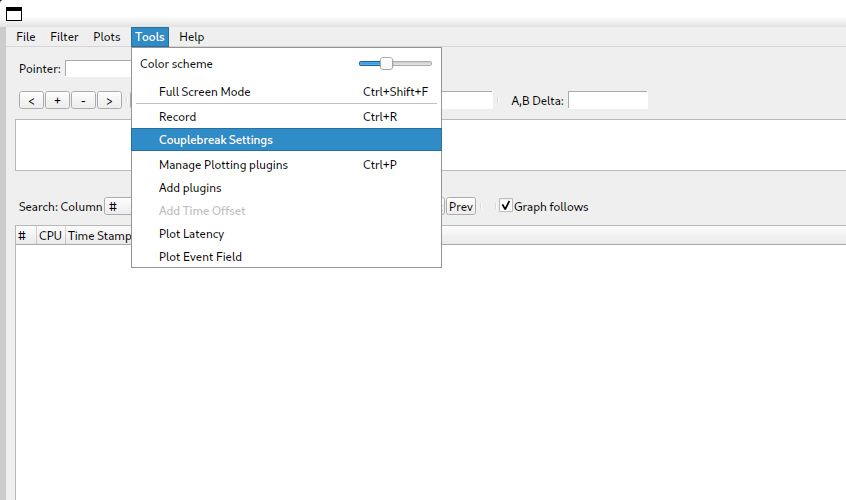
\includegraphics[width=140mm]{img/Modifikace/modif-couplebreak-tools}
    \caption{Submenu tools s modifikací tlačítkem pro konfiguraci Couplebreaku.}
    \label{cbreak-tools}
\end{figure}

\begin{figure}[p]\centering
    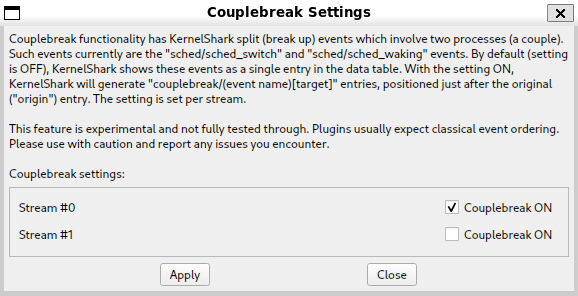
\includegraphics[width=140mm]{img/Modifikace/modif-couplebreak-multiconf}
    \caption{Dva streamy jsou otevřené, v jednom z nich je aktivní Couplebreak.}
    \label{cbreak-multiconf}
\end{figure}

Zaškrtnutím políčka pro nějaký stream v konfiguračním okénku a následným použitím této konfigurace se data ve streamech načtou znovu. Toto také donutí pluginy aktivní v dotyčných streamech, aby se znovu načetly. Pluginy si tak mohou obnovit svůj kontext a použít nová data (tj. s novými záznamy Couplebreak událostí).

Záznamy Couplebreak událostí mohou být filtrovány jednoduchým filtrem stejně jako ostatní události, viz obrázek \ref{cbreak-filter}. Nelze je filtrovat pomocí pokročilých filtrů, ty nejsou podporovány. Záznamy jsou viditelné v seznamu událostí a i v grafu. Je možné, že budou zakrývat záznam své počáteční události, nebo budou naopak zakrývány takovým záznamem. Z hlediska rozlišení událostí to není velký problém, obě události jsou v podstatě to samé, jenom rozdělené. Pro vybrání zakrytého záznamu je pak nejjednodušší jej vybrat v seznamu událostí.

\begin{figure}[p]\centering
    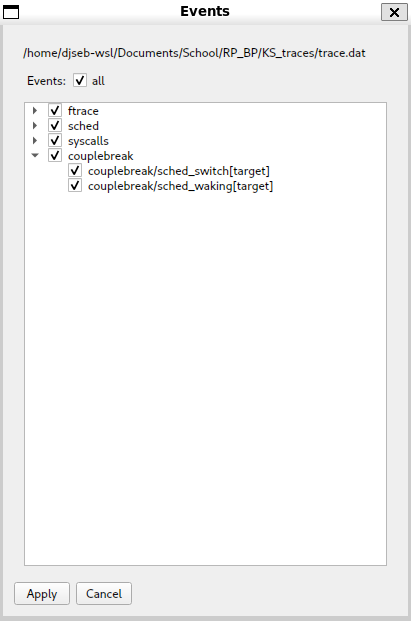
\includegraphics[width=140mm]{img/Modifikace/modif-couplebreak-filter}
    \caption{V jednoduchém filtru lze vybírat i Couplebreak události.}
    \label{cbreak-filter}
\end{figure}

\subsection{Vývojář}

Modifikace se snaží být nerušivou součástí KernelSharku. Pokud budeme někdy chtít dále vyvíjet pro KernelShark, tak lze naše změny třeba nejprve navrhnout pro KernelShark bez aktivního Couplebreaku a až poté se pokoušet o integraci, pokud je nutná. Většinou by pak měl nový kód kontrolovat zda je Couplebreak aktivní přes proměnné ve streamu a měnit chování podle této informace. Samozřejmě existují i vylepšení, pro která nemá taková kontrola smysl, například rozšíření relací o nový datový formát - zde je nutné ukládat data Couplebreaku (alespoň zda byl ve streamu aktivní).

Vývojář pluginů pak může využít Couplebreak API a také kontrolovat přítomnost této modifikace ve streamu a dál tato data využívat. Modifikace by pak měla být respektována vždy, kdy se se očekává nějaký sled událostí a Couplebreak nějakou z nich dokáže dělit. Couplebreak ale může i pomoci s vytvořením kompatibility pro nějaké pluginy. Příkladem mohou být pluginy sched\_events a \emph{Naps}\ref{nappin}. Oba z pluginů potřebují měnit procesy vlastnící nějaké události, aby mohly kreslit své tvary do grafu jednoho procesu. Pokud jsou oba pluginy aktivní bez zapnutého Couplebreaku, tak buď kreslí mezi špatnými záznamy, nebo na špatných místech. Oba totiž pohnuly se záznamy a narušili tak očekávání druhého z nich. S Couplebreakem nemusejí se záznamy hýbat, jelikož pro své potřeby si mohou vybrat záznamy od Couplebreaku.

Následující podsekce pak detailněji píší o hlavních prvcích, se kterými se nejspíše vývojář střetne, pokud bude s Couplebreakem pracovat.

\subsubsection*{Couplebreak API}

K většině operací by měla posloužit nové API, kterou lze používat přes \texttt{\#include}. S její pomocí lze kontrolovat identifikátor události u záznamu události, tj. zjistit, zdali se jedná o Couplebreak záznam. Také lze kontrolovat přítomné události v bitmasce ve streamu - pokud neznáme pozici indikátoru, API ji dokáže uživateli říci. Užitečnou funkcí je pak získání záznamu počáteční události z Couplebreak záznamu, nebo jen získání jména Couplebreak události.

Identifikátory Couplebreak událostí jsou pojmenované konstanty v makrech. Formát jména je \texttt{COUPLEBREAK\_[zkratka]T\_ID}, kde \uv{[zkratka]} je zkrácený název pro událost, pro kterou vytváříme novou Couplebreak událost, a T symbolizuje, že se jedná o cílovou/target událost. Příkladem, pro sched\_waking událost je zkratka \uv{SW}. Celý název konstanty identifikátoru je \uv{COUPLEBREAK\_SWT\_ID}. Existují i makro konstanty pro pozice indikátorů v bitmasce, ale je doporučeno, aby se ke čtení bitmasky či její manipulaci používaly funkce k tomu určené, nikoliv tato makra.

\subsubsection*{Couplebreak ve streamech}

Streamy KernelSharku nyní obsahují následující položky představující stav Couplebreaku:
\begin{itemize}
    \item \texttt{couplebreak\_on} - indikátor zapnutého či vypnutého Couplebreaku ve streamu.
    \item \texttt{n\_couplebreak\_evts} - počet vytvořených typů Couplebreak událostí, tj. pokud se ve streamu vytvořily pouze události pro sched\_switch, bude počitadlo mít hodnotu 1, i kdyby bylo vytvořeno tisíc takových záznamů událostí.
    \item \texttt{couplebreak\_evts\_flags} - bitmaska, která zaznamenává, které typy událostí jsou ve streamu přítomné. Pozice indikátorových bitů lze najít v Couplebreak API. Maska zaznamenává od LSb.
\end{itemize}
Nedoporučuje se měnit jakoukoliv z položek výše, podobně jako se nedoporučuje měnit například původní položku ve streamu, počet opravdových zaznamenaných událostí ve streamu \texttt{n\_events}. Modfikace nemá definované chování, pokud se tyto položky změní. Čtení není nijak omezeno.

Každá funkce v rozhraní streamů může být používána jako dříve, i s Couplebreak událostmi. Pro Couplebreak většinou taková funkce bude pracovat s daty původního záznamu. Druhou možností je, že Couplebreak vytvoří požadované hodnoty na místě. To je hlavní rozdíl oproti normálním záznamům událostí, jelikož ty takovou hodnotu získávají ze souboru s trasovacími daty.

\subsubsection*{Záznamy Couplebreak událostí}

Couplebreak události jsou přidány za běhu programu a nemohou nijak kontrolovat \uv{původní data}, například původní název procesu, kterému událost patří. Dotazy na taková data jsou tak buď nasměrovány na záznamy událostí, kvůli kterým vznikly, nebo vytvořením dat nanovo (např. vytvoření jména události). Toto je způsobeno tím, co je v datech záznamů Couplebreak událostí, speciálně v jejich poli \texttt{offset}, kde není offset do trasovacího souboru, nýbrž ukazatel na původní záznam události. Z toho také vychází, že toto pole se nikdy nesmí pro záznamy Couplebreak událostí měnit. Kromě tohoto pole je zakázáno i jakkoliv měnit pole \texttt{event\_id}, jelikož pro takový záznam je tato změna nevratná. Pokud jakékoliv z těchto dvou polí bude změněno, chování takového záznamu je nedefinováno, záznam lze považovat za rozbitý a již neobsahuje Couplebreak událost.

\subsection{Bugy a chyby}

Záznamy Couplebreak událostí by se neměly účastnit kreslení obdélníků mezi záznamy v grafu, jelikož nepředstavují opravdovou práci, nýbrž důsledek práce někde jinde. KernelShark ale nemá jak rozlišit tyto záznamy a obdélníky se kreslí i pro ně. Vylepšení \emph{NoBoxes} se snaží toto chování opravit, nicméně neumí to dokonale.

Během vývoje KernelSharku dvakrát spadl při opravě CPU pro sched\_waking[target] záznamy. Ačkoliv bug se již dlouho neobjevil, nebyl ani explicitně opraven. Pokud by KernelShark spadl při načítání trasovacích dat, je možné, že příčinou byl Couplebreak.

\section{Rozšíření}

\subsubsection*{Podpora více událostí}
Přirozeným rozšířením této modifikace by bylo rozšíření Couplebreaku o více událostí, případně i o vytváření nějakých počátečních událostí. Existující kód Couplebreak událostí a všeho, co s jich týká, by měl dostatečně nastínit, jak postupovat při takových změnách.

\subsubsection*{Optimalizace průchodů daty při opravě CPU pro sched\_waking}
Couplebreak ve své stávající podobě donutí nasbíraná data, aby byla setříděna dle CPU a času do nějakého pole, ve kterém poté vyhledá konečná CPU pro probouzené události, tzv. opraví CPU. Stejné pole později vytváří ale i později další funkce, které jsou zavolány po naší opravě. Vytváříme tedy pole, které poté zahodíme, ale po chvíli je vytvořeno znovu. Toto rozhodně představuje prostor pro optimalizace.

První možnou optimalizací je prosté neopravování CPU cílových událostí. Zkrátka volání opravy neprovedeme. Tím ale také přijdeme o informaci, kde nakonec byl proces probuzen. Je to ovšem nejjednodušší řešení.

Druhou možností je použít trik podobný hledání záznamů zásobníku v pluginu \emph{Stacklook}. Vytvořili bychom plugin, který cílovým událostem CPU opraví v jednom průchodu při prvním pokusu o kreslení a dále se nevolá, pokud není plugin načten znovu. Nápad to není špatný, ale bylo by nutné pak řešit situace, kdy by některé jiné pluginy nebo části KernelSharku mohly očekávat původní CPU.

Třetí možností je ponořit se vnitřností KernelSharku a upravit místa, kde se pole vytváří a místa, kde zanikají. Pokud bychom opravili CPU, tak bychom si možná mohli na pole uschovat ukazatel a nějakým způsobem ho předat funkcím, které by pak nemusely vytvářet nové setříděné pole. Toto by byla čistá optimalizace a nebylo by nutné oddělovat opravy CPU od Couplebreaku.

\subsubsection*{Couplebreak v datovém streamu}
Streamy mají v současnosti tři proměnné, které dohromady symbolizují stav Couplebreau ve streamu: počet typů vytvořených Couplebreak událostí, indikátor aktivního Couplebreaku a bitmasku vytvořených typů. Navrženým rozšířením je úprava, a to pouze na dvě proměnné. Jelikož máme omezeně mnoho bitů v bitmasce, lze v konstantním čase spočítat i počet vytvořených typů událostí z této proměnné. Tím bychom mohli z datové struktury odstranit počet Couplbreak událostí a místo toho toto číslo vždy rychle spočítat. Pokud bychom se chtěli opravdu omezit na minimum proměnných, bylo by možné použít pouze jednu bitmasku, kde jeden bit by speciálně označoval aktivní Couplebreak.

Toto rozšíření ale není moc užitečné v desktopovém prostředí, kde GUI aplikace obyčejně běží. Streamů KernelShark nevytváří mnoho a tak na paměti moc neušetříme. Není pro nás ani zajímavá časová stopa, protože desktopová prostředí většinou mají i dostatečné zdroje na rychlé výpočty, zvláště pokud se jedná o práci s bity.

Jediným dobrým důvodem pro rozšíření by bylo sjednocení proměnných streamu do jedné struktury. Tím bychom sice paměti nepomohli, ale ve streamu by bylo méně proměnných a stav Couplebreaku by byl více zapouzdřen, než doposud.

\subsubsection*{Funkce \texttt{get\_*\_event\_ids} a širší podpora pro umělé události}
Couplebreak přidal \texttt{get\_couplebreak\_evt\_ids} (\uv{Couplebreak} funkce) do rozhraní streamu. Vytvořena byla proto, že úprava \texttt{get\_all\_event\_ids} (\uv{all} funkce) pro spolupráci s Couplebreakem by způsobila příliš mnoho úprav chování v místech, kde byla použita. Tato použití někdy vůbec nepotřebují o umělých událostech vědět.

S \uv{Couplebreak} funkcí je ale funkcionalita \uv{all} funkce narušena - nyní už nevydá všechny události ve streamu, nýbrž jen všechny události, které nejsou vytvořeny Couplebreakem. Bylo by proto lepší, kdyby \uv{all} funkce byla alespoň přejmenována, aby lépe odrážela svou práci, například na \texttt{get\_all\_original\_event\_ids}. Poté bychom i mohli dodat funkci, která by vrátila opravdu všechny události. Dobré by pak bylo projít celý kód KernelSharku a rozhodnout zdali jsou na místech použití \uv{all} funkce potřeba všechny události, nebo pouze originální události.

Celkově by bylo hezké dodat KernelSharku obecnou podporu pro práci s umělými událostmi, nejen pro události od Couplebreaku. Ten je sice jediným výrazným producentem umělých událostí, ale nemusí tomu tak být napořád, mohou přibýt další vylepšení, která budou umělé události využívat.

\subsubsection*{Rozdělování pouze některých událostí}
Možným rozšířením je rozdělování pouze některých událostí, které bychom si vybrali v konfiguraci. Tím by bylo rozdělování jemnější. Nicméně by také bylo nutné refaktorovat části, které kontrolují aktivní Couplebreak, například pokud by nás zajímalo jenom to, zdali se rozdělují události typu sched\_switch. Zároveň by toto znamenalo indikátory pro každou událost, na což by mohla být opět použita bitmaska.

\subsubsection*{Podpora pokročilých filtrů}
Couplebreak události mohou být filtrovány jen pomocí jednoduchých filtrů. Ale bylo by možné (i příjemné) mít možnost je využít v pokročilých filtrech. S nimi by pak měl uživatel detailnější kontrolu nad zobrazováním záznamů a navíc by tak byla odstraněna tato nesrovnalost vůči ostatním událostem, které tyto filtry podporují.

\section{Kritika}
V této sekci autor kriticky zhodnotí své řešení. Každá kritika má nadpis a popis a dále buď obsahuje obranu proti ní, nebo souhlas s předneseným problémem.

\subsubsection*{Změny ve stream API}
Tato podsekce očekává, že čtenář viděl kód Couplebreaku.

Změna funkcí ve stream API je trochu nepříjemná. Kvůli missed\_events již KernelShark představuje nějaký způsob, jak zpracovávat vlastní umělé události. Couplebreak ale občas potřebuje speciální zpracování a tak je někdy cesta položená KernelSharkem opomíjena. Zpracovávání žádosti na stream API pak prochází přes sekci pro normální událost, pak sekci pro Couplebreak události a až poté se dostane k sekci pro obecné vlastní události, kde by dle původní implementace mělo probíhat zpracování. Couplebreak tak občas nerespektuje záměry kódu, což může čtenáři kódu působit tu trochu nepříjemnosti. Příkladem by mohla být funkce \texttt{tepdata\_dump\_entry}, kdy se zpracování pro Couplebreak stane před switch konstrukcí, ve které se očekávalo zpracování vlastních umělých událostí. Zde je přítomno i vysvětlení, proč je Couplebreak řešen jinak.

\section{Zhodnocení splnění požadavků}
Modifikace není v žádném z otevřených streamů aktivní, dokud není zapnuta skrze nové konfigurační okénko. KernelShark tak vůbec s Couplebreakem nemusí pracovat. Plugin sched\_events také pracuje jako dříve, pokud ve streamu, kde plugin působí, není Couplebreak zapnutý. Jedinou viditelnou změnou, která se koná vždy, je ukládání relací. Zde Couplebreak nutně ukládá, zdali je v nějakém streamu aktivní a každý soubor relace pak tuto informaci obsahuje. Ale načítání relací v původní implementaci nepracuje s Couplebreakem, a pokud je načtena starší relace, Couplebreak je vypnutý. Tím splňujeme obecný požadavek \emph{minimálního vlivu} modifikací. Požadavek \emph{stylové podobnosti} se musí ověřit čtením kódu provedených změn. Rychle lze ale například ověřit, že Couplebreak se snaží používat podobné formáty jmen pro prvky v C kódu a podobné formáty jako v C++ kódu. Požadavek o \emph{chování se jako rozšíření} je též splněn - pokud je někde změna původního chování, je popsána v komentáři, například při opravách CPU u cílových sched\_waking událostí. Navíc Couplebreak vždy kontroluje, zdali je zapnutý, pokud tomu tak není, pak se KernelShark chová jako dříve. Ostatní změny jsou triviálně pouze rozšiřující, jako nová funkce pro stream API, Couplebreak API s novými funkcemi, nebo nové proměnné v datové struktuře streamů.

Vlastní cíle Couplebreak plní, při analýze bylo řešení sestaveno tak, aby cíle splňovalo.
\chapter{Naps}
\label{nappin}
V této kapitole rozebereme plugin pro KernelShark, se kterým budeme schopni v grafu zobrazit dobu mezi přepnutím nějaké úlohy a jejím probouzením od nějakého jiného procesu. Termínem \uv{nap} pak označujeme právě období nečinnosti nějakého procesu. V kapitole se seznámíme s cíli, analýzou řešení, návrhem a použitím tohoto pluginu. Nakonec i řešení kriticky zhodnotíme a představíme návrhy pro rozšíření.

\section{Cíle}

\begin{itemize}
    \item Mezi událostmi sched\_switch procesu P1 a sched\_waking procesu P2, který probouzí P1, se bude vykreslovat obdélník a text. Vykreslený text bude název předchozího stavu P1 před přepnutím. Vykreslený obdélník bude měnit svou barvu dle předchozího stavu.
    \item Plugin musí dostat sched\_waking události do grafů procesů, které jsou těmito událostmi probouzeny, aby mohl své grafické objekty vykreslovat.
    \item Plugin bude spolupracovat s vylepšením Couplebreak. Namísto využívání sched\_waking událostí se využijí cílové události probouzení. Spolupráce musí být automatická, tj. pokud je zapnut Couplebreak, plugin ho používá, a pokud je Couplebreak vypnutý, plugin jej nepoužívá - to vše bez vstupu od uživatele.
    \item Plugin bude možné konfigurovat skrze grafické okénko. Minimální konfigurovatelné nastavení bude maximální počet záznamů viditelných v grafu, než se plugin aktivuje. 
\end{itemize}

\section{Analýza}
Tato sekce zachytí postup postup, kterým se dostaneme k implementaci řešení. Jedná se o techničtější a detailnější analýzu než analýza z kapitoly \emph{Obecná analýza a stanovení požadavků}. Tato sekce bude často odkazovat na plugin Stacklook a jeho analýzu, abychom se vyhnuli zbytečnému opakování.

\subsection{Propojení s KernelSharkem}
Přeskočíme hlubší přemýšlení nad tím, jak připojit plugin do KernelSharku, to jsme již udělali u analýzy kapitoly pluginu Stacklook \ref{lookin-at-stacks} a stejný postup můžeme jednoduše upravit pro naše účely. V rychlosti ale zopakujeme, že plugin s KernelSharkem propojíme pomocí handlerů pro kreslení, vytváření menu nebo načítání dat. Pluginy mají kontext, ve kterém jsou proměnné pro daný plugin globální, takový kontext si sami definujeme. Implementaci propojujícího modulu rozdělíme do C kódu, který se bude starat hlavně o propojení s KernelSharkem a správné přiřazování handlerů, a do C++ kódu, který se bude starat o složitější logiku fungování pluginu.

Jediným opravu podstatným rozdílem bude handler pro načítání událostí. Nyní nebudeme pouze vybírat pro nás zajímavé záznamy událostí, kterými jsou sched\_switch a sched\_waking. Pro události typu sched\_waking je upravíme i tak, že proces, který událost vlastní, změníme z procesu probouzejícího na proces probouzený. Tím budeme pak schopni kreslit obdélníky mezi přepnutím kontextu z procesu až po jeho probouzení. Postup je velmi podobný pluginu sched\_events, který takto přesouvá pro své účely události sched\_switch.

Již zde je jasné, že pluginy si bez Couplebreaku neporadí a budou si vzájemně škodit, budou-li aktivní ve stejném streamu. V kapitole o Couplebreaku jsme sched\_events vylepšili o možnost namísto sched\_switch událostí vybírat události od Couplebreaku. Naps také bude obsahovat kód, který bude schopen Couplebreak využít. Takto bude i pěkně předvedena schopnost Couplebreaku být mostem pro kompatibilitu některých pluginů. Jediné, co my musíme přidat, je kontrola, zdali je ve streamu Couplebreak aktivován, která proběhne před určením událostí, které nás budou zajímat. Pokud je Couplebreak aktivní, tak se nebudeme zajímat o události sched\_waking, nýbrž o události sched\_waking[target]. Takto jsme stejně jako u pluginu sched\_switch odstranili nutnost měnit data trasovaných událostí a plugin žádným dalším pluginům nemůže škodit reorganizací záznamů událostí.

\subsection{Kreslení obdélníků do grafu}
KernelShark dodává API na kreslení objektů, ovšem my bychom nyní chtěli kreslit pomocí dvou záznamů v grafu, nikoli pouze pomocí jednoho, jako u Stacklooku. KernelShark má i takovou situaci vyřešenou pomocí \uv{intervalového kreslení}, tj. kreslení mezi dvěma záznamy, které přirozeně v grafu vytváří nějaký časový interval. Nám pak opět stačí jenom dodat nějakou kreslící funkci s danou signaturou, pomocí níž KernelShark obdélník nakreslí. Narozdíl od Stacklooku ale budeme kreslit obdélníky pouze v grafech procesů, jelikož doba nečinnosti procesu se zřejmě týká jenom tohoto procesu.

\subsection{Nap obdélníky}
Nyní nám už jen stačí obdélníky navrhnout. Název \uv{nap obdélník} označuje právě obdélník vytvořený tímto pluginem. Z cílů nám vychází, že musejí být dostatečně velké pro text a zároveň je dáno, že barva musí být spojena s předchozím stavem. Nejjednodušším řešením zde bude nějaká konstantní mapa předchozích stavů na barvy. Aby byly barvy jednoduše rozlišitelné, tak budeme pracovat s barvami světlými i tmavými. Přidáme ještě barvení vrchní a spodní strany obdélníku podle barvy procesu - k tomu nám pomůže dodatečné vylepšení \emph{Get Colors}. Toto barvení nebude ve výchozím nastavení zapnuto, tj. obdélníky nebudou mít žádné hrany obarvené. Cílem tohoto vedlejšího vylepšení je jak ukázka \emph{Get Colors}, tak o trochu hezčí prezentace obdélníků.

Obdélníky budou pak muset text zobrazovat dle světlosti barvy buď v černé nebo v bílé. Text umístíme někam doprostřed obdélníku. Je možné, že dva záznamy, mezi kterými má být obdélník, budou příliš blízko. Proto budeme text zobrazovat jenom pokud obdélníky budou dostatečně široké, to vypočteme pomocí délky textu k zobrazení. Podobně jako u Stacklooku získáme data pro text z informací v sched\_switch události. Nebudeme ale vytvářet samostatný mini-modul jako u Stacklooku, získání stavu bude pouze součást vytváření obdélníku.

Obdélníky nebudou mít definované interakce s uživatelem, není to součást naších cílů, tedy nebudou reagovat ani na dvojité kliknutí, ani na přejetí kurzorem myši.

\subsection{Konfigurace}
Zde využijeme dělení konfigurace ze Stacklooku na konfigurační objekt a GUI okénko, které je jediným místem pro manipulaci konfiguračního objektu. Také dáme uživateli možnost konfigurovat počet viditelných záznamů v grafu, než se plugin spustí. A podobně jako u Stacklooku přidáme zaškrtávací tlačítko pro použití funkcionalit od \emph{Get Colors}. Žádné další konfigurační možnosti nedodáme, jelikož nejsou potřeba. Pokud sestavíme Naps pro nemodifikovaný KernelShark, tak zaškrtávací políčko nebude součástí konfigurace, nemělo by pak, co měnit.

\subsection{Plugin pro nemodifikovaný KernelShark}

Stejně jako Stacklook, i Naps využije podmíněnou kompilaci pomocí makra \texttt{ifndef} s názvem \texttt{\_UNMODIFIED\_KSHARK}. Zde se bude pouze týkat barvení hran nap obdélníků.

\section{Vývojová dokumentace}

\subsection*{Dokumentace pluginu}
Dokumentace je napsána pro nástroj Doxygen. Dokumentována byla každá funkce i proměnná, ale vygenerovaná dokumentace obsahuje jen prvky veřejné. Pro implementační detaily je doporučeno se podívat do zdrojového kódu. Dokumentace obsahuje i hlavní stránku a stránku s nástinem návrhu.

\subsection*{Struktura projektového adresáře}

Adresář pluginu obsahuje další adresáře. Adresář \uv{src} je pro zdrojový kód a adresář \uv{doc} je pro dokumentaci uživatelskou a dokumentaci technickou. Očekává se, že na této úrovni jsou i adresáře pro sestavení. Na stejné úrovni žije i README, soubor s licencí a nejvyšší CMakeLists.txt. V těchto CMake instrukcích se nastaví proměnné sestavení, například typ sestavení, a případně se zavolá generování dokumentace. CMake instrukce zodpovědné za vytvoření binárního souboru jsou v adresáři se zdrojovým kódem, stejně jako to dělá KernelShark.

\subsection*{Přehled modulů pluginu}

\begin{itemize}
    \item \emph{Propojující modul} - Modul s kódem propojujícím KernelShark a plugin. Obsahem je hlavně kontext pluginu, funkce kontextu, handlery a implementačně pomocné funkce. Součástí tohoto modulu je část s C kódem a implementační část v C++ prvků z hlavičkového C souboru. Právě v \uv{C++ části} (napsaná v C++) se ostatní moduly propojují; zároveň tato část ukládá některá globální data s C++ typy. Soubory modulu jsou \emph{naps.h/c} a \emph{Naps.cpp}.
    \item \emph{Konfigurace} - Modul se skládá ze dvou tříd, konfigurační objekt a konfigurační okénko. Konfigurační objekt obsahuje konfigurační data, která plugin zrovna využívá a je navržen jako singleton. Konfigurační okénko představuje GUI element, kterým se data v konfiguračním objektu manipulují. Soubory modulu jsou \emph{NapConfig.hpp/cpp}.
    \item \emph{Nap obdélníky} - Modul se zajímá vzhled a kreslení nap obdélníků mezi záznamy. Součástí vzhledu je barva, barva vrchní a spodní hrany a text v obdélníku, tj. jeho barva, velikost a obsah. Soubory modulu jsou \emph{NapRectangle.hpp/cpp}.
\end{itemize}

\section{Uživatelská dokumentace}

Tato sekce popíše jak instalovat a používat plugin Naps v KernelSharku a co od něj během běhu očekávat, či na co si dát pozor. Malá ochutnávka fungujícího pluginu je na obrázku \ref{naps-workin}. Styl a i obsah této dokumentace jsou velmi podobné uživatelské dokumentaci Stacklooku, jelikož jsou efektivní a dají se jednoduše poupravit na jiný plugin.

\begin{figure}[p]\centering
    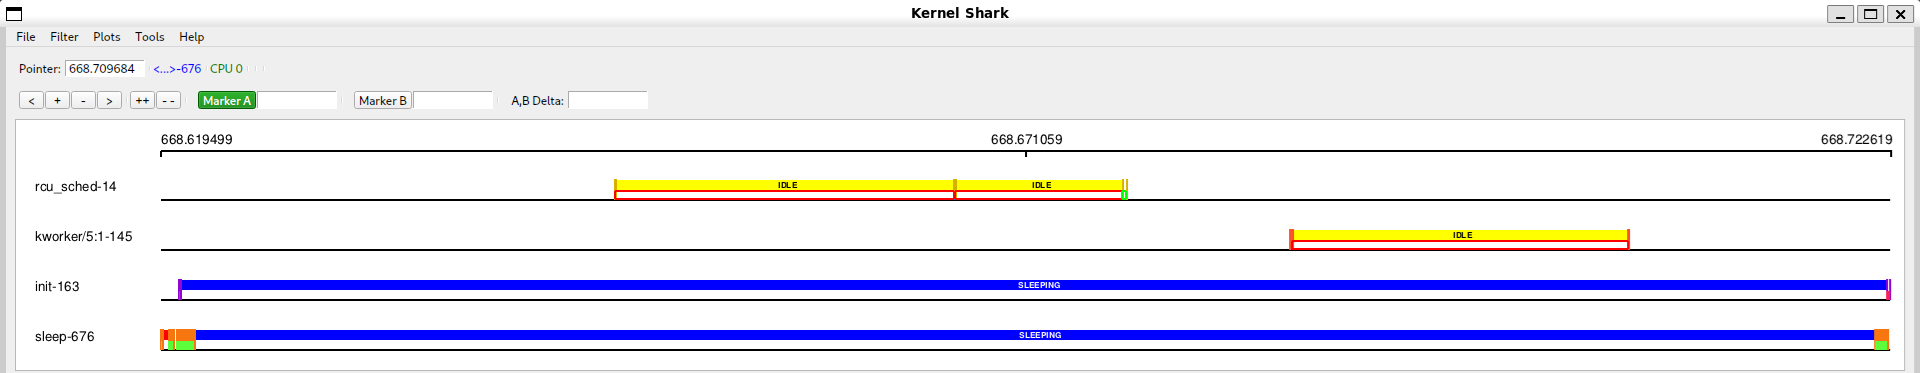
\includegraphics[width=140mm]{img/Naps/NapsWorking}
    \caption{Fungující Naps}
    \label{naps-workin}
\end{figure}

\subsection{Instalace}

\subsubsection{Předpoklady}

\begin{itemize}
  \item CMake verze alespoň 3.1.2.
  \item Pokud chceme plugin využívající modifikovaný KernelShark, pak je nutná verze alespoň 2.4.0-couplebreak. Pokud chceme plugin pro nemodifikovaný KernelShark, pak je nutná verze alespoň 2.3.2.
  \item Závislosti KernelSharku (nalezneme v README repozitáře KernelSharku), zejména Qt6 a traceevent.
  \item Doxygen na technickou dokumentaci.
\end{itemize}

Tento plugin funguje výrazně lépe, pokud je KernelShark modifikovaný. V takovém KernelSharku je plugin plně kompatibilní s oficiálními pluginy, pokud je Couplebreak zapnutý. V případě nemodifikovaného KernelSharku pak tento plugin vyžaduje vypnutí pluginu sched\_events, jinak nebude správně fungovat.

\subsubsection{Sestavení a instalace pouze pluginu}
\begin{enumerate}
  \item V terminálu nastavme pracovní adresář na složku \texttt{build} (pokud ještě neexistuje, pak ji nejlépe vytvořme v kořenovém adresáři projektu).
  \item Spusťme příkaz \texttt{cmake ..}. Pokud hlavní soubor \texttt{CMakeLists.txt} není v nadřazené složce, předejme programu CMake platnou cestu k němu.
    \begin{itemize}
      \item Používáme-li verzi KernelSharku bez modifikací, přidejme do příkazu argument \texttt{-D\_UNMODIFIED\_KSHARK}.
      Sestavení pro nemodifikovaný KernelShark odstraňuje možnost barvit vrchní a spodní hranu obdélníků kreslených pluginem barvou úlohy, které obdélník patří.
      \item Pokud chceme generovat dokumentaci pomocí Doxygenu, přidejme do příkazu argument \texttt{-D\_DOXYGEN\_DOC=1}.
      \item Výchozí typ sestavení je \texttt{RelWithDebInfo}. Chceme-li ho změnit (např. na \texttt{Release}), použijme argument \texttt{-DCMAKE\_BUILD\_TYPE=Release}.
      \item Pokud se v \texttt{/usr/include} nenacházejí hlavičkové soubory knihovny traceevent, použijme argument \texttt{-D\_TRACEEVENT\_INCLUDE\_DIR=[PATH]}, kde \texttt{[PATH]} nahradíme cestou k souborům knihovny.
      \item Pokud se v \texttt{/usr/lib64} nenacházejí sdílené objekty knihovny traceevent, použijme argument \texttt{-D\_TRACEEVENT\_LIBS\_DIR=[PATH]}, kde \texttt{[PATH]} nahradíme cestou ke sdíleným objektům knihovny.
      \item Pokud se soubory Qt6 nenacházejí ve \texttt{/usr/include/qt6}, použijme argument \texttt{-D\_QT6\_INCLUDE\_DIR=[PATH]}, kde \texttt{[PATH]} nahradíme cestou k souborům Qt6.
        \begin{itemize}
          \item Pokyny pro sestavení předpokládají, že zadaný adresář má stejnou vnitřní strukturu jako výchozí možnost (tj. obsahuje složky QtCore, QtWidgets apod.).
        \end{itemize}
      \item Pokud se zdrojové soubory KernelSharku nenachází v \texttt{../KS\_fork/src}, použijme argument \texttt{-D\_KS\_INCLUDE\_DIR=[PATH]}, kde \texttt{[PATH]} nahradíme cestou ke zdrojovým souborům KernelSharku.
      \item Pokud se sdílené knihovny KernelSharku (\texttt{.so} soubory) nenachází ve \texttt{/usr/local/lib64}, použijme \texttt{-D\_KS\_SHARED\_LIBS\_DIR=[PATH]} argument, kde \texttt{[PATH]} nahradíme cestou k sdíleným knihovnám KernelSharku.
    \end{itemize}
  \item Ve složce \texttt{build} spusťme příkaz \texttt{make}.
    \begin{itemize}
      \item Pokud je třeba sestavit jen část pluginu, například pouze dokumentaci, můžeme vybrat konkrétní cíl.
      \item Pouhé spuštění \texttt{make} vytvoří: \emph{plugin} (cíl \texttt{naps}), \emph{symlink} na sdílený objekt pluginu (cíl \texttt{naps\_symlink}) a případně \emph{Doxygen dokumentaci} (cíl \texttt{docs}), pokud tak bylo specifikováno v předchozím kroku.
    \end{itemize}
  \item (\emph{Instalace}): Nahrajme plugin do KernelSharku, buď přes GUI, nebo při spouštění přes CLI s argumentem \texttt{-p} a cestou k symlinku nebo přímo k sdílenému objektu.
    \begin{itemize}
      \item \emph{DŮLEŽITÉ}: Vždy nainstalujme/nahrajme plugin před načtením relace, ve které byl aktivní! Jinak může dojít k neúplnému načtení konfiguračního rozhraní nebo k pádu celého programu.
    \end{itemize}
\end{enumerate}

K odstranění vytvořených binárních souborů použijme \texttt{make clean}.

\subsubsection{Sestavení a instalace pomocí KernelSharku}

\begin{enumerate}
  \item Ujistěme se, že všechny zdrojové soubory (\texttt{.c}, \texttt{.cpp}, \texttt{.h}) pluginu Naps se nacházejí ve složce \texttt{src/plugins} v adresáři projektu KernelShark.
  \item Zkontrolujme, že soubor \texttt{CMakeLists.txt} v této podsložce obsahuje instrukce pro sestavení pluginu (inspirovat se můžeme podle jiných pluginů pro GUI). Pokud chceme sestavovat pro nemodifikovaný KernelShark, upravme tomu odpovídajícím způsobem build skript.
  \item Sestavme KernelShark (pluginy se sestavují automaticky). Lze sestavit i pouze plugin, pokud jsme již předtím vytvořili instrukce sestavení.
  \item (\emph{Instalace}): Spusťme KernelShark. Pluginy sestavené tímto způsobem se načítají automaticky. Pokud by se z nějakého důvodu nenačetly, najděme sdílený objekt stejně jako u ostatních oficiálních pluginů, opět buď přes GUI, nebo přes CLI.
\end{enumerate}

\subsubsection{VAROVÁNÍ - načítání více verzí pluginu}

Máme-li dvě nebo více sestavených verzí pluginu, \emph{NE}načítejme je současně do KernelSharku. Pokud to uděláme, \emph{DOJDE K PÁDU PROGRAMU}. Používejme vždy jen jednu z verzí, \emph{NIKDY OBOJE NAJEDNOU}.

\subsection{Naps v GUI}
\subsubsection{Jak zapnout Naps}

Plugin se zapíná velmi jednoduše. Stačí spustit KernelShark a přejít na položku v panelu nástrojů \texttt{Tools > Manage Plotting plugins}. Pokud byl plugin načten přes příkazový řádek, zobrazí se v seznamu pluginů jako zaškrtnuté políčko se svým názvem. Pokud ne, lze plugin dohledat pomocí tlačítka \texttt{Tools > Add plugin} - stačí nalézt symlink, ale je možné vybrat i samotný soubor sdíleného objektu. Obrázek~\ref{naps-manage-plot-plugs} ukazuje GUI pro zapínání a vypínání pluginů.

\begin{figure}[p]\centering
    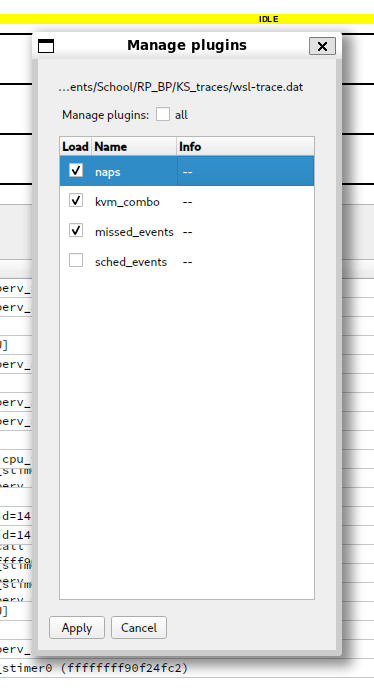
\includegraphics[height=140mm]{img/Naps/NapsManagePlottingPlugins}
    \caption{Okénko se správou pluginů se záznamem pro plugin Naps}
    \label{naps-manage-plot-plugs}
\end{figure}

\subsubsection{Konfigurace}

Konfigurace pluginu může být provedena kdykoliv, i před načtením jakýchkoliv trasovacích dat. Pro otevření konfiguračního okna (viz obrázek~\ref{naps-cfg-window}) stačí v hlavním okně zvolit \texttt{Tools > Naps Configuration}, viz obrázek \ref{naps-cfg-btn}. Vždy může být otevřeno jen jedno konfigurační okno.

\begin{figure}[p]\centering
    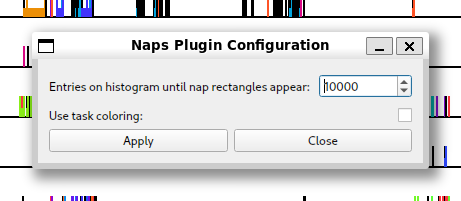
\includegraphics[width=140mm]{img/Naps/NapsConfigWindow}
    \caption{Konfigurační dialog pro plugin Naps}
    \label{naps-cfg-window}
\end{figure}

\begin{figure}[p]\centering
    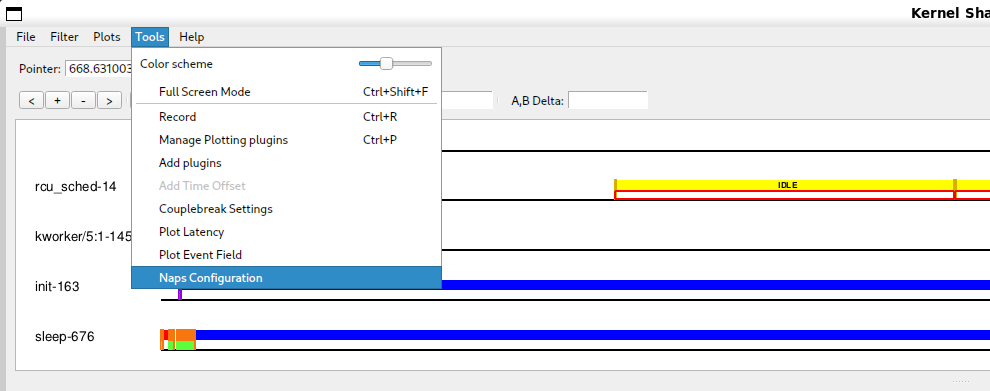
\includegraphics[width=140mm]{img/Naps/NapsConfigButton}
    \caption{Tlačítko na vyvolání konfiguračního dialogu pluginu Naps}
    \label{naps-cfg-btn}
\end{figure}

V konfiguračním dialogu lze pluginu přenastavit dvě věci. První je maximální počet viditelných záznamů v grafu trasování KernelSharku, po jehož překročení plugin nebude nic do grafu kreslit. Pokud je hodnota moc vysoká, pak dovolujeme pluginu strávit pro více událostí více času kreslením. Hodnotu je dobré snížit i tehdy, pokud pociťujeme zpomalení výkonu při kreslení s mnoha záznamy. Výchozí hodnota tohoto nastavení je 10~000 (deset tisíc) záznamů.

Druhou věcí, kterou lze konfigurovat, je barvení vrchní a spodní hrany obdélníků vykreslených pluginem barvou, kterou KernelShark využívá pro daný proces, v jehož grafu je obdélník kreslen (viz obrázek \ref{naps-task-col}). Toto se dá řídit zaškrtávacím políčkem. Ve výchozím nastavení je možnost vypnutá a je použita stejná barva, jako pro vnitřek obdélníku, viz obrázek \ref{naps-def-col}. Pokud byl ale Naps sestaven pro nemodifikovaný KernelShark, toto políčko není v konfiguraci přítomno.

\begin{figure}[p]\centering
    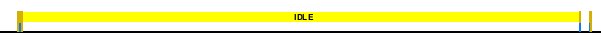
\includegraphics[width=140mm]{img/Naps/NapsDefaultColors}
    \caption{Hrany obdélníku mají stejnou barvu, jako jeho vnitřek}
    \label{naps-def-col}
\end{figure}

\begin{figure}[p]\centering
    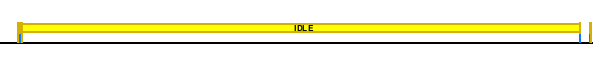
\includegraphics[width=140mm]{img/Naps/NapsTaskLikeColors}
    \caption{Hrany obdélníku používají barvu procesu}
    \label{naps-task-col}
\end{figure}

Kliknutím na tlačítko \texttt{Apply} provedené konfigurační změny potvrdíme a zavřeme tak i dialog. Zobrazí se i zpráva, že změna byla úspěšná, viz obrázek \ref{naps-cfg-succ}. Kliknutím na tlačítko \texttt{Close} nebo na křížek v hlavičce dialogu naopak změny zahodíme, ale poté také zavřeme dialog. Změny takto zahozené se při znovuotevření dialogu nevrátí, hodnoty ke konfiguraci budou stejné, jako hodnoty aktuální konfigurace.

\begin{figure}[p]\centering
    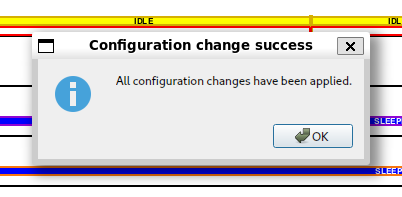
\includegraphics[width=140mm]{img/Naps/NapsConfigSuccess}
    \caption{Dialog signalizuje úspěšnou změnu konfigurace pluginu}
    \label{naps-cfg-succ}
\end{figure}

Plugin si konfiguraci nikam sám neukládá a nespolupracuje s relacemi KernelSharku. Změny provedené před zavřením programu budou muset být znovu nastaveny při dalším otevření.

\subsubsection{Naps v grafech}

Zobrazená \uv{zdřímnutí/naps} procesů jsme již viděli na začátku dokumentace. Tato sekce je trochu více představí.

K zobrazení ob nečinnosti v grafu trasování je nutné mít v tomto grafu grafy procesů. Plugin pak automaticky nakreslí barvené obdélníky mezi událostmi sched\_switch a sched\_waking/sched\_waking[target]. Barva je určena předchozím stavem procesu před přepnutím, například nepřerušitelný spánek je červený. Pokud jsme tak plugin nakonfigurovali, tak vrchní a spodní hrany obdélníků mají stejnou barvu jako proces a jeho záznamy. Pokud je obdélník dostatečně široký, tak je v něm i předchozí stav napsán velkým písmeny celým názvem. Pro příklad obdélníků s různými šířkami se podívejme na obrázek \ref{nap-diff-widths}. S obdélníky nelze nijak interagovat. Obdélníky budou viditelné tak dlouho, dokud dovolí přiblížení dvou záznamů tvořících obdélník, aby byly také viditelné.

![Fig. 8](../images/NapsDifferentWidths.png)
Figure 8.
\begin{figure}[p]\centering
    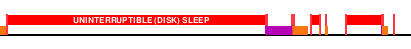
\includegraphics[width=140mm]{img/Naps/NapsDifferentWidths}
    \caption{Obdélníky, které nejsou dostatečně široké, nezobrazí název předchozího stavu}
    \label{nap-diff-widths}
\end{figure}

Níže je seznam předchozích stavů (s anglickými názvy) a barev s nimi spjatých. Přidána jsou i krátká vysvětlení těchto stavů.
\begin{itemize}
  \item Uninterruptible (disk) sleep - červená. Proces čeká na dostupnost zdrojů a nereaguje na signály.
  \item Idle - žlutá. Pro speciální vlákno kernelu, nelze převést do stavu Running.
  \item Parked - oranžová. Pouze pro procesy kernelu, proces se dobrovolně vzdá CPU a označí se tímto stavem, aby mohl být spuštěn později. 
  \item Running - zelená. Proces běží na nějakém CPU.
  \item Sleeping - modrá. Proces čeká na dostupnost zdrojů a reaguje na signály.
  \item Stopped - azurová. Procesu byl zaslán STOP signál.
  \item Tracing stop - hnědá. Proces se zastavil, jelikož je právě trasován či laděn.
  \item Dead - magenta/purpurová. Přechodný stav těsně předtím, než bude proces dealokován.
  \item Zombie - fialová. Proces skončil svou práci a čeká na uklizení rodičovským procesem.
\end{itemize}

\subsection{Bugy a chyby}

Žádné nejsou známy.

\subsection{Doporučení}

Autor níže vypisuje pár doporučení při používání pluginu.
\begin{itemize}
  \item Vždy načtěme Naps před načtením relace. Může to programu ušetřit nepříjemná překvapení.
  \item Pokud chceme dvě verze pluginu, sestavme je do různých adresářů.
  \item Opakujeme, že je doporučeno používat verzi pluginu s KernelSharkem, který obsahuje Couplebreak.
  \item Nedoporučuje se nastavovat příliš vysoký limit záznamů v grafu v konfiguraci. Jinak by plugin mohl používat příliš mnoho paměti kvůli velkému množství naráz kreslených nap obdélníků.
  \item I když relace v KernelSharku fungují, jsou trochu nestabilní. Tento plugin se snaží jejich vnitřní logiku nenarušovat, ale varuje, že pokud plugin není načten předem, mohou nastat neočekávané problémy. Například načtení relace s aktivním pluginem nepřidá do menu \texttt{Tools} odpovídající položku pro vyvolání konfiguračního okna.
\end{itemize}

\section{Rozšíření}
\subsubsection*{Interakce}
Obdélníky fungují dobře, ale možná by bylo dobré přidat nějakou interakci, která by nám o době nečinnosti dala další informace. Například by při přejetí myši mohl informační řádek KernelSharku, nebo nějaká plovoucí vysvětlivka ukázat i rozdíl mezi časem přepnutím a probouzením. Nebo by mohlo být při dvojitém kliknutí zobrazeno okénko, ve kterém jsou nějaké statistiky a detaily o době nečinnosti. Přímé rozšíření tedy nedodáváme, ale tato nastínění snad ukazují, že rozšířit tento jednoduchý plugin lze.

\subsubsection*{Persistentní konfigurace}
Stejně jako u Stacklooku, i zde by bylo pěkné mít schopnost ukládat si konfiguraci z nějaké relace KernelSharku. Zde je problém trochu mírnější, jelikož máme méně věcí, co lze konfigurovat. Ale i tak by bylo lepší nemuset při každém otevření KernelSharku a načtení pluginu manuálně konfiguraci měnit.

\section{Kritika}
Plugin je vcelku malý a autorovi se zdá, že funguje docela bezproblémově. Tu kritiku, kterou má, sdílí se Stacklookem, tj. \emph{Konfigurační singleton} a \emph{Verze pluginu pro nemodifikovaný KernelShark}. I zde platí ty stejné argumenty jako pro Stacklook.

\section{Zhodnocení splnění požadavků}
Plugin zřejmě splňuje první z obecných cíle pluginů, tj. vlastní adresář s instrukcemi k sestavení. Nezávislost na jiných pluginech není dokonale splněna, pokud plugin neběží v prostředí s Couplebreakem. Pokud tomu tak není, tak si s pluginem sched\_events vzájemně škodí a jsou tak na sobě závislé tak, že se vzájemně zakazují. Tomu se bohužel nedá předejít, jelikož není jiný způsob, jak by každý z nich dokázal odvést svou práci.

Jinak jsme v analýze postupovali tak, abychom každý z našich cílů splnili. Navíc jsme nepřišli na žádné další problémy při vytváření řešení. Tím jsme splnili i požadavky vlastní.
\chapter{NUMA Topology Views}
Kapitola se bude zabývat posledním z hlavních vylepšení této práce, tj. přidáním informací o NUMA topologii CPU na systému do KernelSharku. Tato modifikace pak bude hlavně sloužit k vylepšení analýzy trasovacích dat, jelikož budeme jednodušeji schopni určit namáhanou část topologie. Kapitola postupně představí cíle, analýzu řešení, návrh, uživatelskou dokumentaci, návrhy pro rozšíření, kritiku řešení a konečné zhodnocení splnění cílů této modifikace.

%%%%%%%%%%%%%%%%%%%%%%%%%%%%%%%%%%%%%%%%%%%%%%%%%%%%%%%%%%%%%%%%%%%%%%%
\section{Cíle}

\begin{itemize}
    \item Modifikace bude umět zpracovat topologická data z XML souboru vytvořeného programem Hwloc. Z tohoto souboru bude hlavně chtít vyčíst NUMA topologii procesorů.
    \item Zpracovaná topologická data budou zobrazena někde v hlavním okně. Místo zobrazení by mělo dovolovat přirozenou návaznost na CPU grafy. Ty mohou být přeuspořádány tak, aby respektovaly řazení v topologii.
    \item Pokud nemáme topologická data k dispozici pro nějaký stream, nebudeme topologii pro daný stream zobrazovat.
    \item Topologie budou zobrazovány jako stromy.
    \item Každý prvek stromu bude viditelně pojmenován. Pokud by jméno bylo příliš dlouhé, lze použít popisky při najetí myši a jinde zkratky.
    \item Topologické stromy nebudou zobrazovat NUMA uzly, pokud na systému existuje pouze jeden (a NUMA technologie je tedy nepřítomná/nevyužitá).
    \item Topologické stromy budou vždy zobrazovat alespoň jádra v topologii. Ta budou vždy obsahovat alespoň jeden procesor.
    \item Jádra budou zabarvena průměrnou barvou ze svých procesorů. NUMA uzly budou zabarveny průměrnou barvou jader, která jsou součástí NUMA uzlu.
    \item Místo s topologickými stromy bude možné schovat přes GUI prvek.
    \item Modifikace bude mít konfigurační dialog, ve kterém si bude uživatel pro každý otevřený stream schopen vybrat soubor s topologickými daty a typ zobrazení topologie, tzv. \uv{pohled} - buď výchozí, nebo se zobrazením NUMA topologie jako stromu.
    \item Pokud nebude vybrána topologie, ale bude vybrán stromový pohled, bude namísto toho použit výchozí pohled. 
    \item Vybrání souboru topologie s odlišným počtem CPU, než jsou v daném streamu tuto topologii nezobrazí, použije se výchozí pohled a uživatel bude o nesrovnalosti informován.
    \item Modifikace bude uložitelná do relací.
\end{itemize}

\section{Terminologie}
Níže jsou termíny, které tato modifikace používá. Některé termíny jsou přímo inspirované terminologií Hwlocu, některé jsou specifické pouze pro NUMA TV, některé obsahují termíny KernelSharku (ty vysvětleny nebudou).

\begin{itemize}
    \item \emph{Blokový strom} - Bloky vedle sebe, které reprezentují strom. Blok je obdélník a reprezentuje uzel. Hrany jsou reprezentovány dotykem bloků. Nejlépe ukázáno na obrázku \ref{block-tree}.
    \begin{figure}[p]\centering
        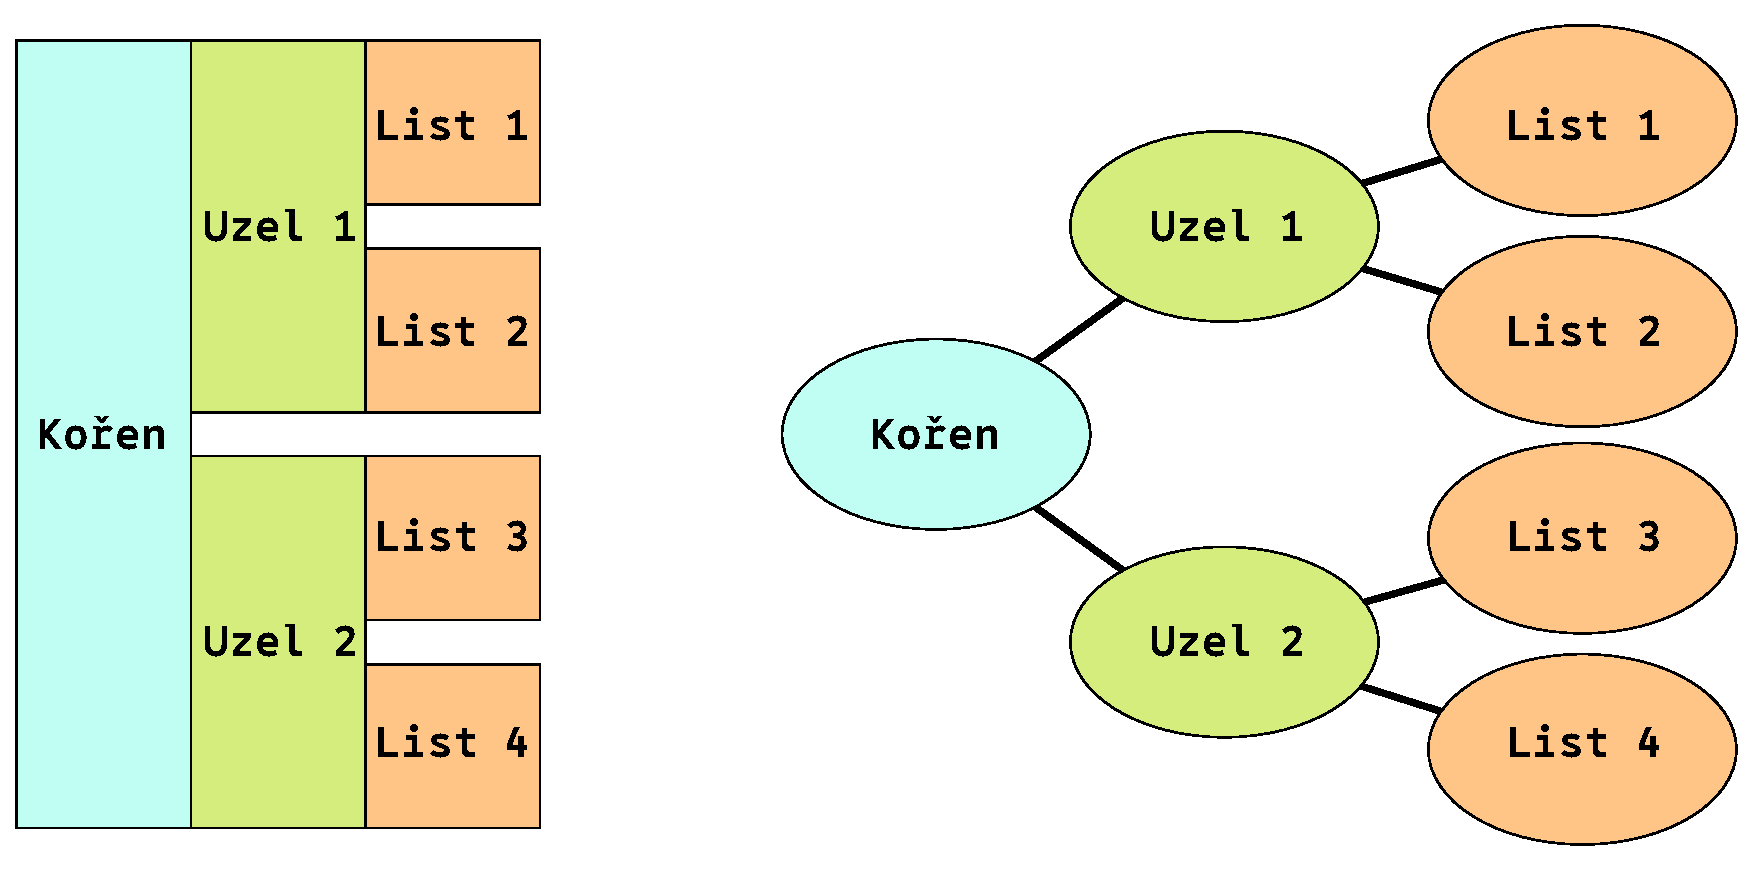
\includegraphics[width=140mm]{img/NUMATV/block-tree.pdf}
        \caption{Blokový strom (vlevo) a klasická grafová reprezentace stromu (vpravo)}
        \label{block-tree}
    \end{figure}
    \item \emph{Zkrácená topologie} - Reprezentace topologie s pouze nejdůležitějšími částmi pro topologickou vizualizaci od NUMA TV. Jedná se o třívrstvou strukturu, kde v první vrstvě jsou logické indexy NUMA uzlů, v druhé vstvě jsou logické indexy jader, ve třetí vrstvě jsou logické indexy procesorů spárovány s OS indexy procesorů.
    \item \emph{C} - Zkratka označující jádro v topologickém stromu, často zobrazováno se svým logickým indexem.
    \item \emph{Jádro} - Topologická struktura v Hwlocu obsahující jeden či více procesorů a která je obsažena v NUMA uzlech. Na systémech bez hyperthreadingu je tento termín zaměnitelný s procesorem.
    \item \emph{GL plocha} - kreslící OpenGL plocha používaná KernelSharkem na kreslení CPU grafů a grafů procesů.
    \item \emph{Logický index} - Index dán části topologie během jejího zkoumání Hwlocem. Společně s typem objektu (PU, jádro, NUMA uzel) pak tvoří unikátní identifikátor komponenty v dané topologii.
    \item \emph{NN} - Zkratka označující NUMA uzel v topologického stromu, často zobrazován se svým logickým indexem.
    \item \emph{NUMA TV} - Zkratka pro \uv{NUMA Topology Views}.
    \item \emph{NUMA TV kontext} - Konfigurační objekt modifikace, který se stará o konfiguraci NUMA TV pro každý otevřený stream, tj. cestu k souboru topologie, kterou má stream načtenou (pokud vůbec), a který typ pohledu chce stream použít při načtené topologii.
    \item \emph{OS index} - Index přidělen hardwarové komponentě operačním systémem. Nerespektuje topologii a pro vizualizace není moc užitečný. Tyto indexy používá KernelShark pro nápisy u CPU grafů, tj. pokud máme zobrazen graf pro CPU 0, tak \uv{0} je OS indexem daného procesoru.
    \item \emph{(Procesorový) modul} - Fyzické místo, kde jsou instalovány procesory (dle Hwlocu). Také součást topologie v Hwlocu, může obsahovat jeden i více NUMA uzlů, zároveň jeden modul může být součástí jednoho i více NUMA uzlů.
    \item \emph{PU/procesor} - Hwloc termín pro to samé, co jsou podle KernelSharku CPU. Mohou být seskupeny v jádru, každé jádro má aspoň jeden PU. PU je zkratka z anglického \uv{processing unit}.
    \item \emph{Topologie} - Struktura s detailní organizací paměťových modulů, procesorů, jiných zařízení na stroji/systému a obsahující nějaké dalších informace, jako například jméno stroje či celková paměť. Tuto strukturu dokáže zachytit Hwloc.
    \item \emph{Úlohová výplň} - Dodatečný prázdný prostor pod topologickým stromem v topologické ploše. Je přítomen pokud KernelShark ukazuje grafy úloh pro nějaký stream.
    \item \emph{Topologický strom} - Skupina Qt objektů, které dohromady tvoří blokový strom bez kořene, jehož první vrstvou jsou NUMA uzly, po nich je vrstva jader, které tvoří listy stromu. Topologické stromy jsou vždy součástí topologické plochy. Topologické stromy NUMA TV vždy vytváří z nějaké zkrácené topologie. Pokud zkrácená topologie nemá více než jeden NUMA uzel, pak se vrstva NUMA uzlů nezobrazuje.
    \item \emph{Vizualizace topologie} - V NUMA TV zaměnitelné s topologickým stromem.
    \item \emph{Topologická plocha} - Qt plocha s topologickým stromem a možnou úlohovou výplní. Je součástí wrapperu topologcké plochy. Lze přímo namapovat na třídu v kódu: \texttt{KsStreamTopoWidget}
    \item \emph{Pohled/typ pohledu} - výčtová třída pro vybrání způsobu zobrazení topologie v KernelSharku. NUMA TV definuje dva pohledy:
    \begin{itemize}
        \item Výchozí pohled, který ignoruje topologii. Pokud jso všechny pohledy nastaveny na výchozí, pak NUMA TV není v hlavním okně aktivní, tj. hlavní okno zobrazuje to samé, co bylo zobrazování před touto modifikací.
        \item \uv{NUMA tree}/stromový pohled, který pro topologii zobrazí topologický strom v topologické ploše.
    \end{itemize}  
    \item \emph{Wrapper topologické plochy} - Nalevo od GL plochy, obsahuje topologickou plochu. Existuje z implementačních důvodů.
\end{itemize}

%%%%%%%%%%%%%%%%%%%%%%%%%%%%%%%%%%%%%%%%%%%%%%%%%%%%%%%%%%%%%%%%%%%%%%%
\section{Analýza}
Tato sekce se pokusí zachytit postup, kterým se dostaneme k implementaci řešení. Jedná se o techničtější analýzu než analýza z kapitoly \emph{Obecná analýza a stanovení požadavků}. Zároveň se někdy odkážeme na Couplebreak a části jeho řešení, abychom se zbytečně neopakovali.

\subsection{Hwloc}
Chtěli bychom-li začít se zobrazováním dat topologie od Hwlocu, musíme si nejprve uvědomit, že se jedná o vylepšení, které přidá ke KernelSharku novou závislost, právě Hwloc. Toho jednoduše docílíme editací souborů sestavení pro CMake. Naštěstí pro nás dává dokumentace Hwlocu \cite{Hwloc-Docs} přímý návod, jak dodání závislosti docílit. Nám tedy stačí řídit se dokumentací a CMake instrukce překopírovat, zkontrolovat a drobně upravit pro KernelShark. Verzi Hwlocu vybereme co možná nejnvější, tj. verzi 2.11.

Na řadu přichází nahrání topologie z XML souboru do datové struktury, se kterou pak může Hwloc pracovat. Dokumentace nám opět pomůže a my můžeme přes Hwloc funkce a makra rovnou načíst XML soubor jako topologii. V té si nejprve získáme všechny OS indexy procesorů/PU a poté si přes každý z nich zjistíme i kterému jádru patří a kterému NUMA uzlu patří. Logické indexy PU, jader a NUMA uzlů si pak uložíme do zkrácené topologie. Abychom neztratili spojení mezi logickými indexy procesorů a jejich OS indexy, uložíme si do zkrácené topologie i OS indexy pro PU. Zkrácenou topologii můžeme implementovat pomocí neseřazených map a indexy můžeme reprezentovat pomocí celých čísel. Zkrácenou topologii použijeme proto, že Hwloc topologie obsahuje informace navíc, které nás u NUMA TV nezajímají, například uspoádání cache pamětí, nebo jméno stroje, na kterém byla topologie zachycena.

\subsection{Hlášení chyb}

Během nahrávání topologie se může stát nějaká chyba, například nebyl XML soubor ve správném formátu. I ve zbytku modifikace pak mohou nastat chvíle, kdy bude potřeba ošetřit a ohlásit nějakou chybovou či informační situaci. KernelShark sám výjimky nevyhazuje, namísto toho používá zprávy v terminálu nebo informační dialogy. NUMA TV bude používat návratové kódy a psaní do terminálu pro hlášení nějak zajímavých situací, jako třeba chyb.

\subsection{Konfigurační dialog}
\label{numatv-cfg-subsec}

Poté, co jsme schopni pracovat s Hwlocem a získat si pro nás zajímavá data, se můžeme začít soustředit vytvoření konfigurace NUMA TV. Začneme GUI pro uživatelskou interakci s konfigurací. Zde si můžeme i rozmyslet, co bude součástí konfigurace, kterou bude tento dialog měnit.

Všimněme si podobností s konfigurací pro Couplebreak \ref{cbreak-cfg-subsec}. I v této modifikaci chceme mít nastavení pro každý stream zvlášť. Můžeme se tedy konfiguračním dialogem Couplebreaku inspirovat a pozměnit jenom to, co pro každý ze streamů konfigurujeme. Naše cíle vyžadují alespoň konfigurovatelnou cestu k XML souboru topologie a typ pohledu, tj. \uv{jak naložit s načtenou topologií}.

Pohledy navíc cíle definují dva, výchozí a stromový. Výchozí pohled už z názvu napovídá, že bude výchozí hodnotou konfigurace pro pohledy. Pohledy můžeme implementovat přes rádiová tlačítka, pak budeme schopni mít vybranou jen jednu možnost pro nějakou skupinu tlačítek.

Výběr XML souboru lze zjednodušit použitím souborového dialogu od Qt a filtrovat pro soubory s příponou \texttt{.xml}. My pak jenom musíme vytvořit nějaké vybírací \texttt{Select} tlačítko, kterým souborový dialog vyvoláme. Ze souborového dialogu pak uložíme cestu k souboru XML jako textový řetězec. Ten pak uživateli zobrazíme, aby bylo jasné, že nějaká topologie byla vybrána. Na vymazání vybrané cesty pak dodáme tlačítko \texttt{Clear}. Výchozí hodnotou cesty k souboru bude přirozeně prázdný text. 

Speciální pozornost dáme tlačítku \texttt{Apply}. To totiž nejenže změny aplikuje, ale před aplikací i zkontroluje některé požadavky, které cíle požadují. Pokud je vybrán stromový pohled, ale nebyl vybrán topologický soubor, pak konfigurace vynutí pohled výchozí, jelikož není co zobrazovat ve stromovém pohledu. Pokud vybereme soubor s topologií o N CPU, ale stream, kterému toto konfigurujeme má M CPU a zároveň M se nerovná N, pak konfigurace opět použije výchozí pohled a uživatel bude o nevhodném souboru topologie informován na chybovém výstupu. Tlačítko \texttt{Cancel} může fungovat jako dřív, tedy prostě dialog zavře bez použití změn.

Tlačítko vyvolávající konfigurační dialog umístíme vedle tlačítka pro konfigurační okéno Couplebreaku, tj. do submenu \texttt{Tools}.

\subsection{Konfigurace NUMA TV}

V předchozí podsekci jsme si už trochu seznámili s tím, jak se bude konfigurace chovat, hlavně z grafického pohledu. Nyní se zamyslíme nad tím, jak by se měla chovat mimo grafické prostředí.

Nejprve se zamyslíme nad tím, jak reprezentovat pohledy. My implementujeme jenom stromový pohled na NUMA topologii, ale teoreticky jich může být více, například pohled na procesorové moduly. Proto pohledy implementujeme jako výčtový typ. Tak se omezíme jen na nějakou konečnou množinu hodnot a budeme mít kódu zřetelněji popsané speciální číselné hodnoty.

Dokud uživatel nezmění konfiguraci v dialogu z výchozích hodnot, pak NUMA TV nebude ukládat žádnou konfiguraci pro stream, jelikož by to bylo zbytečné. Pokud ale uživatel vybere validní XML soubor s topologií, pak se situace mění. Aplikace konfigurace pak donutí NUMA TV vytvořit novou konfiguraci pro stream, včetně interpretace topologického XML sobuoru Hwlocem. Po ní nám zbyde zkrácená topologie, kterou také uložíme do konfigurace pro stream. Z toho nám vyplývá, že datová struktura konfigurace NUMA TV pro nějaký stream bude obsahovat prvky pro uložení cesty k XML souboru, uložení typu pohledu a uložení zkrácené topologie.

Pokud uživatel vymaže v konfiguračním dialogu cestu k topologickému souboru, pak není konfigurace pro stream potřeba. Pro nás to znamená návrat k výchozím hodnotám konfigurace (i kdyby byl vybrán stromový pohled, tak bez cesty k souboru topologie toto NUMA TV změní na výchozí pohled). Abychom zbytečně neukládali nepotřebnou konfiguraci, tak ji v této situaci smažeme.

Dalším problémem, co vyřešíme, je aktualizace topologie. Ta se stane, když uživatel změní cestu k topologickému souboru a nebo změní typ pohledu v konfiguračním dialogu a změny aplikuje. Pokud změní cestu, pak lze považovat starou konfiguraci topologie za zbytečnou a tak ji smažeme. Můžeme ji pak kompletně nahradit novou konfigurací. Pokud se změnil jen pohled, pak změníme jen ten. V každém případě ale požádáme  NUMA TV o překreslení topologických vizualizací (vizualizační část je popsána v nižší sekci \ref{numatv-grt}). Pokud je topologie nějak nevalidní (případy popsány v sekci o konfiguračním dialogu výše \ref{numatv-cfg-subsec}), pak návratovým kódem rozhodneme, jak se má KernelShark zachovat tj. jestli má do terminálu napsat nějakou chybovou zprávu.

Nakonec, namísto ukládání konfigurací ke každému streamu zvlášť si pořídíme manažera konfigurací, tzv. NUMA TV (konfigurační) kontext. Ten si bude pro každý stream pamatovat jeho specifickou konfiguraci. Krom toho bude mít i API pro přidávání, odebírání, a aktualizaci konfigurací pro každý stream. Jelikož mezi streamy mohou být \uv{díry}, tj. ne každý stream musí mít aktivní NUMA TV konfiguraci, bude nejlepší i toto vyřešit mapou, klidně i nesetříděnou.

\subsection{Grafická reprezentace topologie/GRT}
\label{numatv-grt}
[TODO: tohle] %%% Turing-head |vvv|
Topostrom (barvy a interaktivita, vzhled topostromu celkově)...

CPU grafy a grafy úloh...

cpuReDraw + taskReDraw...

Reorganizace grafů dle topologie...

Místo pro GRT (+ velikost + nemožnost scrollovat + updateGeom)...

Spolupráce s filtry...

Schovávání topologie...

\subsection{Životnosti}
Vše patří KsTraceGraph...

Vše umírá v napsaných konstruktorech správně...

\subsection{Relace}
Relace implementujeme mnohem snadněji než u Couplebreaku. NUMA TV uloží pod identifikátor streamu vybraný typ pohledu a cestu k XML souboru (nebo žádnou cestu neuloží v případě nevybraného souboru v konfiguraci). Inspirovat se můžeme ostatním kódem pro ukládání relace, například pro ukládání Markerů A a B. A stejně se inspirujeme i pro načítání NUMA TV z relačního souboru.

Nyní zbývá vybrat momenty, kdy ukládat NUMA TV a hlavně kdy relační data pro modifikaci načítat. Nelze načítat kdykoliv, jelikož bychom jinak nezastihli vykreslení CPU grafů, tedy i jejich možnou reorganizaci, což by vizualizaci úplně pokazilo. Načítat relační data proto budeme před načtením grafu, abychom vykreslení CPU stihli. Ukládání není závislé na pořadí ukládání ostatních částí relace, ale kvůli symetrii s načítáním jej zařadíme před ukládání grafů.

%----------------------------------------------------------------------

\subsection{Zamítnutá alternativní řešení}
Tato část je souhrnem několika nápadů, které se objevily během vymýšlení řešení či během implementace, ale byly nakonec zavrženy z různých důvodů. Představen bude jak návrh řešení, tak důvod zamítnutí.

\subsubsection*{Konfigurační kontext jako singleton}
Až moc dlouho jako prototyp, velmi nebezpečný vzor...

\subsubsection*{Kreslení stromu do OpenGL plochy}
Příšerné, nikdy to tak nedělejme...

\subsubsection*{Graf vytvořen přes QTreeWidget}
Nedostatečné schopnosti a layout nebyl vhodný, reimplementace by byla šílená

\subsubsection*{Zobrazení procesorů a stroje v topologickém stromě}
Zbytečné, ačkoliv stream to aspoň ukotvoval jako strom - nicméně více místa = více radosti...

\subsubsection*{Vlastní zpracování XML souboru}
Pro humor, tohle by byla prostě šílenost...

\subsubsection*{Topologie jako součást datové struktury streamu}
Zbytečné omezení na jazyk C...

\subsubsection*{Topologické zobrazení přítomno neustále}
Zbytečné plýtvání místem...

\subsubsection*{Skládání částí stromu}
Zbytečně komplikované, zbytečná fnkcionalita, která se jen plete pod nohy existujícímu řešení přes menu, ale měla i svá plus...

%%%%%%%%%%%%%%%%%%%%%%%%%%%%%%%%%%%%%%%%%%%%%%%%%%%%%%%%%%%%%%%%%%%%%%%
\section{Vývojová dokumentace}
Cíle/úvod této sekce...

\subsection{Modifikované a nové soubory}
Modifikace používá značku \texttt{NUMA TV} v ohraničujících komentářích pro změny. Níže je abecedně seřazený seznam souborů spojených s modifikací spolu s krátkým popiskem změn či novinek uvnitř souboru.
\begin{itemize}
    \item \emph{(src/)CMakeLists.txt} -
    \item \emph{KsMainWindow.cpp/hpp} - 
    \item \emph{KsNUMATopologyViews.cpp/hpp} -
    \item \emph{KsPlotTools.cpp/hpp} - 
    \item \emph{KsSession.cpp/hpp} -
    \item \emph{KsTraceGraph.cpp/hpp} - 
    \item \emph{KsWidgetsLib.cpp/hpp} -
\end{itemize}

\subsection{Struktura modifikace}
Velké dělení na \emph{Konfiguraci} a \emph{Vizualizaci}. Vše vlastí objekt KsTraceGraph, kromě konfiguračního dialogu, který je vázán jenom na hlavní okno KernelSharku hierarchií oken.

Dělení Konfigurace:
\begin{itemize}
    \item \emph{Konfigurační kontext} -
    \item \emph{Konfigurační dialog} -
    \item \emph{Vytváření zkrácených topologií z Hwlocu} -
    \item \emph{Dotazy na topologii} -
    \item \emph{Relace} -
\end{itemize}

Dělení Vizualizace (modul je i jeden grafický prvek):
\begin{itemize}
    \item \emph{Topologický strom} -
    \item \emph{Prostor pro topologický strom} -
    \item \emph{Skrývající tlačítko} -
    \item \emph{Přerovnání CPU} -
\end{itemize}

%%%%%%%%%%%%%%%%%%%%%%%%%%%%%%%%%%%%%%%%%%%%%%%%%%%%%%%%%%%%%%%%%%%%%%%
\section{Uživatelská dokumentace}

\begin{code}

\subsection{Konfigurace}

To access NUMA TV's confguration, navigate to `Tools > NUMA Topology Views`
button in the toolbar. If no stream was loaded, an error pop-up will be shown
and nothing will happen otherwise.

With a loaded stream, the NUMA TV configuration dialog will be shown,
with a brief explanation of what to do in this window and in the lower half will be
a list of opened streams' NUMA TV configurations, namely what topology file to
load data from and what type of topology view should be used for this stream.
There are also two buttons, "Clear" and "Select...". Clear clears current
configuration's selected topology file (just the filepath to it, not the file
itself). Select button will open up a file dialog, which either starts in the user's
Documents directory or in the directory of the currently applied topology file
(applied = program already loaded this topology file and uses it for a stream).

At the very bottom are two buttons, "Apply" and "Close". Close will ignore any
changes to the configuration done in the window and close the dialog. Apply will
attempt to either create or update chosen stream's topology configuration with
the chosen values.

Beware that if the chosen topology in a file has a different amount of PUs than
KernelShark detected CPUs in its trace file, creation or update of this topology
configuration is ignored (old values remain or the default choice of no topology
file and DEFAULT view). Topology configuration changes will also be ignored if
no actual topology file was chosen (cleared the path or it has been deleted in
between choosing it and applying the changes), yet the NUMA tree view was set.

Applying an empty filepath current configuration of a stream and program will
default to using DEFAULT view with no topology file.

Currently, only NUMA topology tree view is supported, along with the DEFAULT view,
which does what KernelShark always has.

Reopening the configuration dialog will show applied configuration values
(currently in use by the program).

See figure 2 for a session where no topologies are loaded and figure 3 for
a session where one topology is loaded.

![Figure 2](./images/numatv-2.png)
Figure 2.

![Figure 3](./images/numatv-3.png).
Figure 3.

\subsection{GUI}

\subsubsection{Kde najít NUMA TV}

NUMA Topology Views are at first glance not present in the program. This is by
design, as the modification is supposed to be hidden until needed. To see the
modification in action, first open a stream. Then, open and use the configuration
dialog as outlined above.

The wrapper topology widget will be shown if at least one stream requested a
non-DEFAULT topology view. If any CPUs are shown on the GL widget, there will
also be a topology tree present for the streams that requested a NUMA tree view.
Streams configured to use the DEFAULT view only have blank spaces in as their
topology widget. 

\subsubsection{Topologický strom}
The topology tree is a block tree, which is vertically starts at the top of the
start of CPU graphs in the GL widget and vertically ends at the last of those
graphs. If there are only tasks being drawn, there will be blank white space
instead. The topology tree will include only nodes relevant to the CPUs shown in
the GL widget (so if out of 8 CPUs, only 3 are marked as to show their graphs,
then the topology tree will be constructed with cores and NUMA nodes of those
three CPUs). If the topology has only single NUMA node detected (in which case
there is no actual NUMA topology present), the node will be hidden (only Cores
will be visible).

If more streams are opened, each tree starts at its respective stream's CPU
graphs.

Core nodes of the tree will be colored the average color of its CPUs (these colors
are defined by KernelShark), NUMA nodes are colored from averages of core node
colors. If a color is deemed too dark, white text is used for their labels,
otherwise the nodes use black text color.

\subsubsection{Synchronizace rolování s plochou grafu}

While the wrapper topology widget sits in a scrollable area, to retain consistency with
KernelShark's method of scrolling vertically through a graph, no mouse wheel events
are processed by it. Instead, the scrolling area moves the same amount as GL widget's
scrolling area, when its vertical scrollbar's value changes.

If KernelShark's main window is too narrow, a horizontal scroll bar also appears, but
at that point, it is recommended to resize the main window of the program.

\subsubsection{Přeuspořádání CPU grafů}

If a topology determined that CPUs adhere to a different ordering than OS indices indicate,
NUMA TV will rearrange the CPU graphs in the GL widget to properly connect to the topology tree
of a stream. In DEFAULT view, KernelShark orders CPUs by their OS indices, with a NUMATREE view,
they are ordered by their NUMA node's logical index, then their core's logical index and lastly
by their logical index (i.e. a sorted sequence could look like (0, 0, 20), (0, 0, 60), (0, 1, 1),
(1, 5, 2), (1, 5, 3), where first number in the vector is NUMA node's logical index, followed
by the core's logical index, ending with a PUs logical index).

KernelShark graph will still label CPUs with their OS indices.

Rearrangements may happen only if a non-DEFAULT view is chosen for a stream and rearrange CPU
graphs only of that stream. A rearrangament may happen any time the CPU graphs are redrawn.

See figure 4 for a stream with CPU graphs ordered by OS indices, then compare with figure 5's
reordered CPU graphs.

![Figure 4](./images/numatv-4.png)
Figure 4.

![Figure 5](./images/numatv-5.png)
Figure 5.

\subsubsection{Skrývající tlačítko}

Hide button is a green button on the left of the wrapper topology widget. Clicking on it
hides the wrapper topology widget along with all topology trees (figure 6). Clicking on
it again makes the wrapper topology widget and its trees visible again (figure 7).
Accompanied with hidden/shown states are characters on the button: ">" for hidden
and "<" for shown.

This button is shown only if there's at least one stream requesting a non-DEFAULT topology view.
Upon any load of topology requesting a non-DEFAULT view, the wrapper topology widget is not
hidden (figure 7).


![Figure 6](./images/numatv-6.png)
Figure 6.

![Figure 7](./images/numatv-7.png)
Figure 7.

\subsubsection{Plovoucí popisky uzlů stromu}

Hovering with the mouse cursor over a topology tree node and letting it stay there for a little while
shows a tooltip with the current node's full name, e.g. hovering over a node labeled 'NN 1' will show
"NUMA Node 1" (figure 8).

Purpose of this is to allow short labels for the nodes, while preserving a quick way for the user to
understand what a certain node is.

![Figure 8](./images/numatv-8.png)
Figure 8.

\subsection{Popora relací}

NUMA Topology Views configuration can be saved in a session using new API of KsSession. Each stream has their view and
topology file path saved.

Importing a session automatically draws topology widgets, if any are desired.

\subsection{Nová API}

NUMA TV presents among new classes also four new global functions:
- `numatv_count_PUs`: This function counts the number of PUs in a brief topology.
- `numatv_count_cores`: This function counts the number of cores in a brief topology.
- `numatv_filter_by_PUs`: This functions returns a brief topology, where its members contain or
  are PUs given in a vector. This function is very useful when some CPU graphs are hidden - by
  filtering the brief topology, we get a brief topology where only the visible CPUs are present,
  same for their cores and NUMA nodes.
- `numatv_stream_wants_topology_widget`: This function checks whether a stream is requesting a
  non-DEFAULT view in its configuration in the given NUMA TV context

Any other API that got introduced is either explicitly labeled with "numatv" ot "topology" or "topo"
somewhere (letters can be uppercase). If not, it belongs to a type with that label or a header
file with that label.

Use carefully.

\subsection{Bugy a chyby}

Qt may sometimes complain about recursive call when clicking the Load button in the configuration dialog. This has no bearing
on actual work of the program, as Qt makes sure to detect these calls and stop them. This may happen if the Load button
is clicked too fast.

No others are known to the author. But the modification was rather significant and there are always possibilites something
went wrong in secret.
\end{code}

%%%%%%%%%%%%%%%%%%%%%%%%%%%%%%%%%%%%%%%%%%%%%%%%%%%%%%%%%%%%%%%%%%%%%%%
\section{Rozšíření}
Cíle/úvod této sekce...

\subsubsection*{Více pohledů}
Package view, něco spešl, ALE nutno vyřešit \ref{nerozšiřitelnost}...

\subsubsection*{Konfigurační dialogy by mohly být zobecněny}
Couplebreak a NUMA TV mají v podstatě stejnou šablonu, bylo by lepší ji zobecnit...

%%%%%%%%%%%%%%%%%%%%%%%%%%%%%%%%%%%%%%%%%%%%%%%%%%%%%%%%%%%%%%%%%%%%%%%
\section{Kritika}
V této sekci autor kriticky zhodnotí své řešení. Každá kritika má nadpis a popis a dále buď obsahuje obranu proti ní, nebo souhlas s předneseným problémem.

\subsubsection*{Nerozšiřitelnost}
\label{nerozšiřitelnost}
Primárně pro NUMA topologii, nedostatečný vhled dopředu pro další viewtypes, ať už v GUI nebo v konfiguraci...

\subsubsection*{Nevhodné umístění třídy \texttt{KsStreamNUMATopology}}
Mělo to mít vlastní soubor nebo do NUMATV souboru...

\subsubsection*{Kostrbaté vložení závislosti do \texttt{CMakeLists.txt} KernelSharku}
Ale je to oficiální...

\subsubsection*{Nemožnost upravovat aktivní topologie}
Místo toho create + delete only...

\subsubsection*{Výjimky místo návratových kódů}
KernelShark to tak nedělá...

\subsubsection*{Porušení SRP}
Zas tak moc ne, furt to zlepšuje analýzu, nicméně chápu, odkud míříme...

\subsubsection*{Orientace a velikost popisků topologického stromu}
Mohlo by být větší/tučné/vertikální/rotované...

\subsubsection*{Barva uzlů topologického stromu}
Avg z toho většinou udělá šedou/hnědou... mohlo by být jinak...

\subsubsection*{Konfigurace a widget v oddělených mapách}
Nemuselo by být, ale dává smysl...

\subsubsection*{Malá interaktivita topologického zobrazení}
A to vůbec nevadí...ale samozřejmě by šlo něco takového dodat...

\subsubsection*{Používání C ukazatelů}
Pravda, nejsou moc bezpečné, ale KernelShark to často dělá a Qt si s nimi umí poradit...

\subsubsection*{Dialogy namísto standardních výstupů}
Grafická aplikace, ne nutně bude vždy uživatel mít přístup k jejímu terminálovému výstupu...

%%%%%%%%%%%%%%%%%%%%%%%%%%%%%%%%%%%%%%%%%%%%%%%%%%%%%%%%%%%%%%%%%%%%%%%
\section{Zhodnocení splnění požadavků}
Obecné požadavky hlavně + možná nějaká porušení + splnění vlastních cílů...
\chapter{Dodatečná vylepšení}

Jedná se o vylepšení, která vznikla kvůli ostatním vylepšením, nebo jako rychlá zlepšení chování KernelSharku. Pro každé z nich bude stručně popsán návrh, řešení, použití a případná varování.

\section{Aktualizace kódu zaškrtávacích políček}

Nejpřímějším zlepšením byla aktualizace grafického kódu, aby využíval novější Qt API pro zaškrtávací políčka. V nové API se nahrazuje funkce QCheckBox::stateChanged za QCheckBox::checkStateChanged. Hlavní změna se týká v argumentu značící zaškrtnutí - předtím stačilo dodat argument typu int, od Qt 6.7 ale nová funkce vyžaduje jednu z enumerovaných možností specifických pro QCheckBox.

Aktualizace nakonec spočívala pouze v nahrazení signálu stateChanged na checkStateChanged a použití výčtových hodnot (dle původního čísla) namísto pouze celých čísel.

KernelShark původně vynucoval v sestavení Qt verze 6.3, nyní vyžaduje alespoň verzi 6.7, aby mohl využít novější signál pro zaškrtávací políčka.

Změněné soubory: nejvyšší \emph{CMakeLists.txt} KernelSharku (v KS\_fork adresáři), \emph{KsTraceViewer.hpp/cpp}, \emph{KsCaptureDialog.hpp/cpp}, \emph{KsMainWindow.hpp/cpp}. Značkou modifikace v C++ kódu a CMake instrukcích je UPDATE CBOX STATES.

Pokud mají v plánu vývojáři KernelSharku či jeho pluginů dále pracovat s KernelSharkem, musejí tedy použít alespoň Qt6 verze 6.7.0.

\section{Zpřístupnění barev užívaných v grafu}

Modifikace je pouze zpřístupnění barevných tabulek, které KernelShark používá pro streamy, CPU a procesy. Díky zpřístupnění pak mohou tyto tabulky využívat i jiné části programu, nebo i pluginy. Jedná se o pouhé získání const reference na objekty využívané uvnitř KsGLWidget objektu. Přirozeně se jedná o malé úpravy, lokalizované v souboru \emph{KsGLWidget.hpp}, se kódovou značkou GET COLORS. K využití této modifikace stačí mít přístup k GL objektu a zavolat nové metody.

K využití přes pluginy se váže varování - pokud si KernelShark uloží do relace plugin, který využívá tuto modifikaci, ale načtení pluginu není dokonalé, program při první snaze o získání hodnoty z jakékoliv z tabulek spadne. Plugin je nedokonale načten vždy, pokud KernelShark načte relaci s daným pluginem, ale ten není předem explicitně načten uživatelem, tedy skrze argumenty při spouštění, nebo přes GUI. Další možnou podmínkou je, že plugin není postaven jako oficiální pluginy KernelSharku, tedy během sestavování KernelSharku samotného. Takto lze postavit například plugin Stacklook. Tato podmínka ovšem nebyla rigorózně otestována a je to spíše pouhá domněnka. Chybě se lze vyhnout třemi způsoby: buď uživatel vždy explicitně načte plugin, nebo plugin nebude tyto tabulky využívat, nebo bude obsahovat výchozí hodnotu, kterou použije namísto tabulek při načtení z relace - barevné tabulky se využijí až později, například až pokud si je uživatel zapne v konfiguraci pluginu.

Tuto modifikaci využívají pluginy Stacklook a Naps pro barvy procesů, a modifikace NUMA Topology Views pro barvy procesorů.

Příklad: Stacklook nabízí možnost barvit tlačítka dle barev procesů, kterým patří, viz obrázek \ref{obr01:modif-get-colors}.

\begin{figure}[p]\centering
    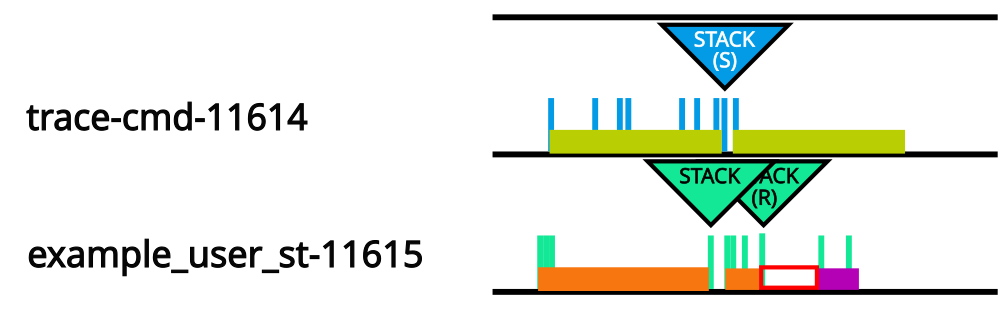
\includegraphics[width=140mm]{img/Modifikace/modif-get-colors-traced.png}
    \caption{Stacklook tlačítko využívá barvu, kterou KernelShark udělil procesu.}
    \label{obr01:modif-get-colors}
\end{figure}

\section{Reakce objektů v grafu na přejetí myší}

Tato modifikace dodala všem potomkům třídy KsPlot::PlotObject, jednodušeji plot-objekty, veřejnou metodu pro reakci na přejetí myší a redefinovatelnou privátní virtuální metodu, kterou veřejná metoda volá pro viditelný objekt. Privátní metoda má výchozí definici prázdnou. Krom toho je dodána detekce přejetí přes plot-objekt v grafu a reakce na přejetí. Toto chování bylo vsunuto na konec zpracování události pohybu myši a funguje podobně jako detekce dvojitého kliknutí. Soubory s modifikací: \emph{KsPlotTools.hpp} s novými metodami a \emph{KsGLWidget.cpp} pro vsunutou detekci a reakci. Kódová značka modifikace je MOUSE HOVER PLOT OBJECTS.

Nabízí se zde otázka, zdali je toto dostatečně výkonná implementace - myš se pohybuje často, objektů může být mnoho. Řešení musí vždy projít všechny plot-objekty a u každého se rozhodnout, zdali reagovat na myš či nikoliv. Při praktickém použití s rozumnými limity pro zobrazované plot-objekty (nedává smysl neustále zobrazovat tlačítka Stacklooku nad každým prvkem grafu, vedlo by to k přemíře informací) nenastaly problémy a nejvíc program zpomaloval objem dat a náhlé vykreslování objektů, nikoliv práce této modifikace. Pokud bude ale objektů příliš mnoho, výkon může být ovlivněn. Proto se optimalizace výkonu nechává jako \emph{rozšíření} této práce. Inspirací může být nahrazení lineárního prohledávání for-cyklem vyhledáváním přes souřadnice, tedy přes nějaké mapování souřadnic na objekty na těchto souřadnicích.

Tuto modifikaci používá hlavně plugin Stacklook.

\section{Měnitelné nápisy v hlavičce grafu}

Tato modifikace přidává do souborů \emph{KsTraceGraph.hpp/cpp} veřejnou funkci, s níž lze přepsat obsah informačního řádku KernelSharku. Jedná se o funkci typu setter, pouze nastaví hodnoty nápisů v informačním řádku.

K použití stačí mít k dispozici KsTraceGraph objekt. Pak se dá s modifikací pracovat i v pluginech a jiných částech KernelSharku.

V kódu lze tuto modifikaci nalézt pod značkou PREVIEW LABELS CHANGEABLE.

I zde se objevuje bug ze sekce o zpřístupnění barev využívaných v grafu, jenom se tentokrát netýká tabulek, nýbrž informačního řádku. Zde ale nelze spoléhat na nějaké výchozí hodnoty, tedy uživatel musí buď plugin vždy explicitně načíst, nebo nepoužívat plugin využívající tuto modifikaci.

Příklad použití: tlačítka Stacklooku (v červeném kroužku) žádají na přejetí myší o zobrazení několika prvků zásobníku kernelu, viz obrázek \ref{obr02:modif-preview-labels-changeable}.

\begin{figure}[p]\centering
    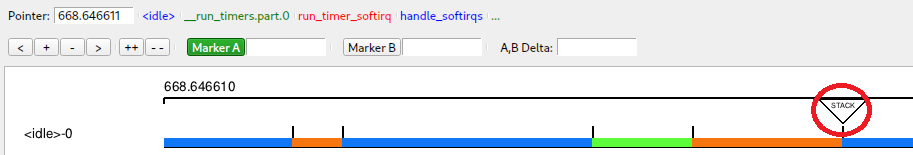
\includegraphics[width=140mm]{img/Modifikace/modif-preview-labels-changeable.png}
    \caption{Při přejetí kurzorem myši se vlevo nahoře informační řádek změní.}
    \label{obr02:modif-preview-labels-changeable}
\end{figure}

\section{NoBoxes}

Jak popsala čtvrtá kapitola, chtěli bychom některé záznamy při vykreslování ignorovat, jinak se nám může zobrazovat falešná práce v grafu. Vykreslování obdélníků mezi záznamy se děje při každém vykreslení grafu. Ovlivnit obdélníky dokáže v této chvíli máloco. Pracuje se zde s biny, tedy sdruženími jednoho či více záznamů. V binech se pak nelze na mnoho spolehnout, ale můžeme použít data viditelnosti, u kterých KernelShark ukládá i nastavení speciálních chování. Viditelnost binu lze ovlivnit viditelností záznamů, které sdružuje.

Vylepšení vytvořilo novou masku viditelnosti pro záznamy, KS\_DRAW\_TASKBOX\_MASK. Tato maska značí, zdali se záznam účastní kreslení mezi-záznamových obdélníčků. Vykreslování pak bylo upraveno tak, že pokud bin využije viditelnost záznamu, který se nemá účastnit kreslení obdélníků, pak obdélníky budou při kreslení tento bin ignorovat.

Na výběr záznamů, kteří budou masku používat, byl vytvořen plugin pro tuto modifikaci, nese název NoBoxes. V jeho kódu jsou zapsány události, na jejichž záznamy má být maska použita, plugin pak lze zapínat a vypínat jako každý jiný. Pokud plugin není načten, modifikace nemá na chod KernelSharku vliv.

Příklad fungujícího vylepšení je na obrázku \ref{obr04:modif-noboxes-good}. Oproti minulému obrázku (obrázek~\ref{obr03:modif-noboxes-bad}) ubylo několik obdélníků a graf nyní odpovídá skutečné práci.

\begin{figure}[p]\centering
    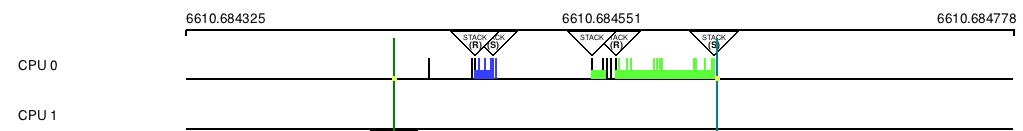
\includegraphics[width=140mm]{img/Modifikace/modif-noboxes-good}
    \caption{Vylepšení donutí některé obdélníky k tomu, aby nebyli nakresleny.}
    \label{obr04:modif-noboxes-good}
\end{figure}

Problém tohoto vylepšení je ale právě vykreslování obdélníků. Vykreslování se děje často a použitá implementace tohoto vylepšení při grafických změnách v hlavním okně KernelSharku obdélník vykreslí i pokud by neměl projít novým filtrováním. Při častých změnách pak nastává problikávání obdélníků. Oprava byla označena za rozšíření, jelikož objem práce k tomuto dodatku byl odhadnut na příliš velký a vytvořený best-effort přístup funguje, ačkoliv ne dokonale.

\chapter*{Závěr}
\addcontentsline{toc}{chapter}{Závěr}

Cíle/úvod této kapitoly...

\section{Shrnutí práce}

\section{Zhodnocení splněných požadavků}                             %%% ZÁVĚR + možná rozšíření

%%% Seznam použité literatury
%%% Seznam použité literatury (bibliografie)
%%%
%%% Pro vytváření bibliografie používáme biblatex. Ten zpracovává
%%% citace v textu (např. makro \cite{...}) a vyhledává k nim literaturu
%%% v souboru literatura.bib.
%%%
%%% Podívejte se na nastavení biblatexu v souboru thesis.tex.

%%% Vytvoření seznamu literatury. Pozor, pokud jste necitovali ani jednu
%%% položku, seznam se automaticky vynechá.

% Dovolíme položkám trochu vyčuhovat přes pravý okraj.
\def\bibfont{\hfuzz=2pt}

\printbibliography[heading=bibintoc,title=Literatura]

%%% Kdybyste chtěli bibliografii vytvářet ručně (bez biblatexu), lze to udělat
%%% následovně. V takovém případě se řiďte normou ISO 690 a zvyklostmi v oboru.

% \begin{thebibliography}{99}
%
% \bibitem{lamport94}
%   {\sc Lamport,} Leslie.
%   \emph{\LaTeX: A Document Preparation System}.
%   2. vydání.
%   Massachusetts: Addison Wesley, 1994.
%   ISBN 0-201-52983-1.
%
% \end{thebibliography}


%%% Obrázky v práci
%%% (pokud jich je malé množství, obvykle není třeba seznam uvádět)
\listoffigures

%%% Tabulky v práci (opět nemusí být nutné uvádět)
%%% U matematických prací může být lepší přemístit seznam tabulek na začátek práce.
% \listoftables

%%% Použité zkratky v práci (opět nemusí být nutné uvádět)
%%% U matematických prací může být lepší přemístit seznam zkratek na začátek práce.
% \chapwithtoc{Seznam použitých zkratek}

%%% Součástí doktorských prací musí být seznam vlastních publikací
\ifx\ThesisType\TypePhD
\chapwithtoc{Seznam publikací}
\fi

%%% Přílohy k práci, existují-li. Každá příloha musí být alespoň jednou
%%% odkazována z vlastního textu práce. Přílohy se číslují.
%%%
%%% Do tištěné verze se spíše hodí přílohy, které lze číst a prohlížet (dodatečné
%%% tabulky a grafy, různé textové doplňky, ukázky výstupů z počítačových programů,
%%% apod.). Do elektronické verze se hodí přílohy, které budou spíše používány
%%% v elektronické podobě než čteny (zdrojové kódy programů, datové soubory,
%%% interaktivní grafy apod.). Elektronické přílohy se nahrávají do SISu.
%%% Povolené formáty souborů specifikuje opatření rektora č. 72/2017.
%%% Výjimky schvaluje fakultní koordinátor pro zavěrečné práce.
\appendix
\chapter{Přílohy}

\section{První příloha}

\end{document}
